\documentclass[]{book}
\usepackage{lmodern}
\usepackage{amssymb,amsmath}
\usepackage{ifxetex,ifluatex}
\usepackage{fixltx2e} % provides \textsubscript
\ifnum 0\ifxetex 1\fi\ifluatex 1\fi=0 % if pdftex
  \usepackage[T1]{fontenc}
  \usepackage[utf8]{inputenc}
\else % if luatex or xelatex
  \ifxetex
    \usepackage{mathspec}
  \else
    \usepackage{fontspec}
  \fi
  \defaultfontfeatures{Ligatures=TeX,Scale=MatchLowercase}
\fi
% use upquote if available, for straight quotes in verbatim environments
\IfFileExists{upquote.sty}{\usepackage{upquote}}{}
% use microtype if available
\IfFileExists{microtype.sty}{%
\usepackage{microtype}
\UseMicrotypeSet[protrusion]{basicmath} % disable protrusion for tt fonts
}{}
\usepackage[margin=1.5in]{geometry}
\usepackage{hyperref}
\hypersetup{unicode=true,
            pdftitle={IQSS Workshops},
            pdfborder={0 0 0},
            breaklinks=true}
\urlstyle{same}  % don't use monospace font for urls
\usepackage{natbib}
\bibliographystyle{apalike}
\usepackage{color}
\usepackage{fancyvrb}
\newcommand{\VerbBar}{|}
\newcommand{\VERB}{\Verb[commandchars=\\\{\}]}
\DefineVerbatimEnvironment{Highlighting}{Verbatim}{commandchars=\\\{\}}
% Add ',fontsize=\small' for more characters per line
\usepackage{framed}
\definecolor{shadecolor}{RGB}{248,248,248}
\newenvironment{Shaded}{\begin{snugshade}}{\end{snugshade}}
\newcommand{\KeywordTok}[1]{\textcolor[rgb]{0.13,0.29,0.53}{\textbf{#1}}}
\newcommand{\DataTypeTok}[1]{\textcolor[rgb]{0.13,0.29,0.53}{#1}}
\newcommand{\DecValTok}[1]{\textcolor[rgb]{0.00,0.00,0.81}{#1}}
\newcommand{\BaseNTok}[1]{\textcolor[rgb]{0.00,0.00,0.81}{#1}}
\newcommand{\FloatTok}[1]{\textcolor[rgb]{0.00,0.00,0.81}{#1}}
\newcommand{\ConstantTok}[1]{\textcolor[rgb]{0.00,0.00,0.00}{#1}}
\newcommand{\CharTok}[1]{\textcolor[rgb]{0.31,0.60,0.02}{#1}}
\newcommand{\SpecialCharTok}[1]{\textcolor[rgb]{0.00,0.00,0.00}{#1}}
\newcommand{\StringTok}[1]{\textcolor[rgb]{0.31,0.60,0.02}{#1}}
\newcommand{\VerbatimStringTok}[1]{\textcolor[rgb]{0.31,0.60,0.02}{#1}}
\newcommand{\SpecialStringTok}[1]{\textcolor[rgb]{0.31,0.60,0.02}{#1}}
\newcommand{\ImportTok}[1]{#1}
\newcommand{\CommentTok}[1]{\textcolor[rgb]{0.56,0.35,0.01}{\textit{#1}}}
\newcommand{\DocumentationTok}[1]{\textcolor[rgb]{0.56,0.35,0.01}{\textbf{\textit{#1}}}}
\newcommand{\AnnotationTok}[1]{\textcolor[rgb]{0.56,0.35,0.01}{\textbf{\textit{#1}}}}
\newcommand{\CommentVarTok}[1]{\textcolor[rgb]{0.56,0.35,0.01}{\textbf{\textit{#1}}}}
\newcommand{\OtherTok}[1]{\textcolor[rgb]{0.56,0.35,0.01}{#1}}
\newcommand{\FunctionTok}[1]{\textcolor[rgb]{0.00,0.00,0.00}{#1}}
\newcommand{\VariableTok}[1]{\textcolor[rgb]{0.00,0.00,0.00}{#1}}
\newcommand{\ControlFlowTok}[1]{\textcolor[rgb]{0.13,0.29,0.53}{\textbf{#1}}}
\newcommand{\OperatorTok}[1]{\textcolor[rgb]{0.81,0.36,0.00}{\textbf{#1}}}
\newcommand{\BuiltInTok}[1]{#1}
\newcommand{\ExtensionTok}[1]{#1}
\newcommand{\PreprocessorTok}[1]{\textcolor[rgb]{0.56,0.35,0.01}{\textit{#1}}}
\newcommand{\AttributeTok}[1]{\textcolor[rgb]{0.77,0.63,0.00}{#1}}
\newcommand{\RegionMarkerTok}[1]{#1}
\newcommand{\InformationTok}[1]{\textcolor[rgb]{0.56,0.35,0.01}{\textbf{\textit{#1}}}}
\newcommand{\WarningTok}[1]{\textcolor[rgb]{0.56,0.35,0.01}{\textbf{\textit{#1}}}}
\newcommand{\AlertTok}[1]{\textcolor[rgb]{0.94,0.16,0.16}{#1}}
\newcommand{\ErrorTok}[1]{\textcolor[rgb]{0.64,0.00,0.00}{\textbf{#1}}}
\newcommand{\NormalTok}[1]{#1}
\usepackage{longtable,booktabs}
\usepackage{graphicx,grffile}
\makeatletter
\def\maxwidth{\ifdim\Gin@nat@width>\linewidth\linewidth\else\Gin@nat@width\fi}
\def\maxheight{\ifdim\Gin@nat@height>\textheight\textheight\else\Gin@nat@height\fi}
\makeatother
% Scale images if necessary, so that they will not overflow the page
% margins by default, and it is still possible to overwrite the defaults
% using explicit options in \includegraphics[width, height, ...]{}
\setkeys{Gin}{width=\maxwidth,height=\maxheight,keepaspectratio}
\IfFileExists{parskip.sty}{%
\usepackage{parskip}
}{% else
\setlength{\parindent}{0pt}
\setlength{\parskip}{6pt plus 2pt minus 1pt}
}
\setlength{\emergencystretch}{3em}  % prevent overfull lines
\providecommand{\tightlist}{%
  \setlength{\itemsep}{0pt}\setlength{\parskip}{0pt}}
\setcounter{secnumdepth}{5}
% Redefines (sub)paragraphs to behave more like sections
\ifx\paragraph\undefined\else
\let\oldparagraph\paragraph
\renewcommand{\paragraph}[1]{\oldparagraph{#1}\mbox{}}
\fi
\ifx\subparagraph\undefined\else
\let\oldsubparagraph\subparagraph
\renewcommand{\subparagraph}[1]{\oldsubparagraph{#1}\mbox{}}
\fi

%%% Use protect on footnotes to avoid problems with footnotes in titles
\let\rmarkdownfootnote\footnote%
\def\footnote{\protect\rmarkdownfootnote}

%%% Change title format to be more compact
\usepackage{titling}

% Create subtitle command for use in maketitle
\providecommand{\subtitle}[1]{
  \posttitle{
    \begin{center}\large#1\end{center}
    }
}

\setlength{\droptitle}{-2em}

  \title{IQSS Workshops}
    \pretitle{\vspace{\droptitle}\centering\huge}
  \posttitle{\par}
    \author{}
    \preauthor{}\postauthor{}
      \predate{\centering\large\emph}
  \postdate{\par}
    \date{October 2019}

\usepackage{booktabs}

\usepackage{epsfig}
\usepackage{epstopdf}
\usepackage{rotate}
\usepackage{graphicx}
\usepackage{hyperref}
\usepackage{alphalph}
\usepackage{caption}
\usepackage[hang,flushmargin]{footmisc}
\usepackage{framed}
\usepackage{xcolor}
\usepackage{verbatim} 

\usepackage{bm}
\setcounter{MaxMatrixCols}{20}
\newcommand{\Var}{\mathrm{Var}}
\newcommand{\SD}{\mathrm{SD}}
\newcommand{\Cov}{\mathrm{Cov}}
\newcommand{\fx}{f({\bf x})}
\newcommand\R{{\textsf R~}}
\newcommand\Rst{\textsf{RStudio}}

% spacing between environments
\usepackage{amsthm}
\makeatletter
\def\thm@space@setup{%
  \thm@preskip=15pt plus 2pt minus 4pt
  \thm@postskip=\thm@preskip
}
\makeatother


% Title format
\usepackage{titling}
\pretitle{\Huge\sffamily}
\posttitle{\par\vskip 0.5em}
\predate{\LARGE\sffamily}
\postdate{\par}

\urlstyle{tt}

\begin{document}
\maketitle

{
\setcounter{tocdepth}{1}
\tableofcontents
}
\chapter*{Introduction}\label{introduction}
\addcontentsline{toc}{chapter}{Introduction}

\section*{Table of Contents}\label{table-of-contents}
\addcontentsline{toc}{section}{Table of Contents}

Materials for the \href{http://dss.iq.harvard.edu}{Data Science
Services} statistical software workshops from the
\href{http://iq.harvard.edu}{Institute for Quantitative Social Science}
at Harvard.

\begin{enumerate}
\def\labelenumi{\arabic{enumi}.}
\tightlist
\item
  \href{./Rintro.html}{R Introduction}
\item
  \href{./Rmodels.html}{R Regression Models}
\item
  \href{./Rgraphics.html}{R Graphics}
\item
  \href{./RDataWrangling.html}{R Data Wrangling}
\item
  \href{./PythonIntro.html}{Python Introduction}
\item
  \href{./PythonWebScrape.html}{Python Web-Scraping}
\item
  \href{./StataIntro.html}{Stata Introduction}
\end{enumerate}

These workshops are a work-in-progress, please provide feedback! Email:
\href{mailto:help@iq.harvard.edu}{\nolinkurl{help@iq.harvard.edu}}

\section*{Authors and Sources}\label{authors-and-sources}
\addcontentsline{toc}{section}{Authors and Sources}

The contents of these workshops are the result of a collaborative effort
from members of the Data Science Services team at IQSS over many years.
The main contributors are: Ista Zahn, Steve Worthington, Jinjie Liu, and
Yihan Wang.

\part{R}\label{part-r}

\chapter{R Introduction}\label{r-introduction}

\textbf{Topics}

\begin{itemize}
\tightlist
\item
  Assignment
\item
  Function arguments
\item
  Finding help
\item
  Reading data
\item
  Filtering rows, selecting columns, and arranging data
\item
  Conditional operations
\item
  Saving data
\end{itemize}

\section{Setup}\label{setup}

\subsection{Software \& materials}\label{software-materials}

You should have R and RStudio installed --- if not:

\begin{itemize}
\tightlist
\item
  Download and install \href{http://cran.r-project.org}{R}
\item
  Download and install
  \href{https://www.rstudio.com/products/rstudio/download/\#download}{RStudio}
\end{itemize}

Download materials:

\begin{itemize}
\tightlist
\item
  \href{http://tutorials.iq.harvard.edu/R/Rintro.zip}{Download workshop
  materials}
\item
  Extract materials from \texttt{Rintro.zip} and move to your desktop.
\end{itemize}

Start RStudio and create a new project:

\begin{itemize}
\tightlist
\item
  On Windows click the start button and search for RStudio. On Mac
  RStudio will be in your applications folder.
\item
  In Rstudio go to \texttt{File\ -\textgreater{}\ New\ Project}.
\item
  Choose \texttt{Existing\ Directory} and browse to the \texttt{Rintro}
  directory.
\item
  Choose \texttt{File\ -\textgreater{}\ Open\ File} and select the blank
  version of the \texttt{.Rmd} file.
\end{itemize}

\subsection{Goals}\label{goals}

Class Structure and Organization:

\begin{itemize}
\tightlist
\item
  Ask questions at any time. Really!
\item
  Collaboration is encouraged - please spend a minute introducing
  yourself to your neighbors!
\end{itemize}

This is an introductory R course:

\begin{itemize}
\tightlist
\item
  Assumes no prior knowledge of R
\item
  Relatively slow-paced
\item
  The workshop covers R basics, the R package ecosystem, and practice
  reading files and manipulating data in R
\item
  A more general goal is to get you comfortable with R so that it seems
  less scary and mystifying than it perhaps does now. Note that this is
  by no means a complete or thorough introduction to R! It's just enough
  to get you started.
\end{itemize}

As an example project we will analyze the popularity of baby names in
the US from 1960 through 2017. Among the questions we will answer using
R are:

\begin{itemize}
\tightlist
\item
  In which year did your name achieve peak popularity?
\item
  How many children were born each year?
\item
  What are the most popular names overall? For girls? For Boys?
\end{itemize}

\section{R Interfaces}\label{r-interfaces}

There are many different ways you can interact with R. See the
\href{http://tutorials.iq.harvard.edu/DataScienceTools/DataScienceTools.html}{Data
Science Tools workshop notes} for details.

For this workshop we will use RStudio; it is a good R-specific
integrated development environment (IDE) that mostly just works.

We will also use Rmarkdown --- a type of R file that allows you to
combine plain text with R code. It is easy to later convert Rmarkdown
into MS Word, LaTeX, a pdf, or webpage.

\section{Exercise 0}\label{exercise-0}

The purpose of this exercise is to give you an opportunity to explore
the interface provided by RStudio (or whichever GUI you've decided to
use). You may not know how to do these things; that's fine! This is an
opportunity to figure it out.

Also keep in mind that we are living in a golden age of tab completion.
If you don't know the name of an R function, try guessing the first two
or three letters and pressing TAB. If you guessed correctly the function
you are looking for should appear in a pop up!

\begin{center}\rule{0.5\linewidth}{\linethickness}\end{center}

\begin{enumerate}
\def\labelenumi{\arabic{enumi}.}
\tightlist
\item
  Try to get R to add 2 plus 2.
\end{enumerate}

\begin{Shaded}
\begin{Highlighting}[]
\NormalTok{##}
\end{Highlighting}
\end{Shaded}

\begin{enumerate}
\def\labelenumi{\arabic{enumi}.}
\setcounter{enumi}{1}
\tightlist
\item
  Try to calculate the square root of 10.
\end{enumerate}

\begin{Shaded}
\begin{Highlighting}[]
\NormalTok{##}
\end{Highlighting}
\end{Shaded}

\begin{enumerate}
\def\labelenumi{\arabic{enumi}.}
\setcounter{enumi}{2}
\tightlist
\item
  R includes extensive documentation, including a manual named ``An
  introduction to R''. Use the RStudio help pane. to locate this manual.
\end{enumerate}

\section{R basics}\label{r-basics}

Set your working directory so you don't have to type the full path names
to your data and other files

\begin{Shaded}
\begin{Highlighting}[]
  \CommentTok{# set the working directory}
  \CommentTok{# setwd("~/Desktop/Rintro") # UNIX-based}
  \CommentTok{# setwd("C:/Users/Desktop/Rintro") # MS Windows}
\end{Highlighting}
\end{Shaded}

\subsection{Function calls}\label{function-calls}

The general form for calling R functions is

\begin{Shaded}
\begin{Highlighting}[]
\NormalTok{## FunctionName(arg.1 = value.1, arg.2 = value.2, ..., arg.n - value.n)}
\end{Highlighting}
\end{Shaded}

Arguments can be matched by name; unnamed arguments will be matched by
position.

\subsection{Assignment}\label{assignment}

Values can be assigned names and used in subsequent operations

\begin{itemize}
\tightlist
\item
  The ``gets'' \texttt{\textless{}-} operator (less than followed by a
  dash) is used to save values
\item
  The name on the left gets the value on the right.
\end{itemize}

\begin{Shaded}
\begin{Highlighting}[]
\KeywordTok{sqrt}\NormalTok{(}\DecValTok{10}\NormalTok{) ## calculate square root of 10; result is not stored anywhere}
\NormalTok{x <-}\StringTok{ }\KeywordTok{sqrt}\NormalTok{(}\DecValTok{10}\NormalTok{) }\CommentTok{# assign result to a variable named x}
\end{Highlighting}
\end{Shaded}

Names should start with a letter, and contain only letters, numbers,
underscores, and periods.

\subsection{Asking R for help}\label{asking-r-for-help}

You can ask R for help using the \texttt{help} function, or the
\texttt{?} shortcut.

\begin{Shaded}
\begin{Highlighting}[]
\KeywordTok{help}\NormalTok{(help)}
\end{Highlighting}
\end{Shaded}

The \texttt{help} function can be used to look up the documentation for
a function, or to look up the documentation to a package. We can learn
how to use the \texttt{stats} package by reading its documentation like
this:

\begin{Shaded}
\begin{Highlighting}[]
\KeywordTok{help}\NormalTok{(}\DataTypeTok{package =} \StringTok{"stats"}\NormalTok{)}
\end{Highlighting}
\end{Shaded}

\section{Getting data into R}\label{getting-data-into-r}

R has data reading functionality built-in -- see e.g.,
\texttt{help(read.table)}. However, faster and more robust tools are
available, and so to make things easier on ourselves we will use a
\emph{contributed package} called \texttt{readr} instead. This requires
that we learn a little bit about packages in R.

\subsection{Installing and using R
packages}\label{installing-and-using-r-packages}

A large number of contributed packages are available. If you are looking
for a package for a specific task,
\url{https://cran.r-project.org/web/views/} and \url{https://r-pkg.org}
are good places to start.

You can install a package in R using the \texttt{install.packages()}
function. Once a package is installed you may use the \texttt{library}
function to attach it so that it can be used.

Install the \href{https://www.tidyverse.org/}{tidyverse} suite of
packages and the \texttt{readr} package:

\begin{Shaded}
\begin{Highlighting}[]
\CommentTok{# install.packages("tidyverse")}
\KeywordTok{library}\NormalTok{(tidyverse)}
\CommentTok{# install.packages("readr")}
\KeywordTok{library}\NormalTok{(readr)}
\end{Highlighting}
\end{Shaded}

\subsection{Readers for common file
types}\label{readers-for-common-file-types}

In order to read data from a file, you have to know what kind of file it
is. The table below lists functions that can import data from common
plain-text formats.

\begin{longtable}[]{@{}ll@{}}
\toprule
Data Type & Function\tabularnewline
\midrule
\endhead
comma separated & \texttt{read\_csv()}\tabularnewline
tab separated & \texttt{read\_delim()}\tabularnewline
other delimited formats & \texttt{read\_table()}\tabularnewline
fixed width & \texttt{read\_fwf()}\tabularnewline
\bottomrule
\end{longtable}

\textbf{Note} You may be confused by the existence of similar functions,
e.g., \texttt{read.csv} and \texttt{read.delim}. These are legacy
functions that tend to be slower and less robust than the \texttt{readr}
functions. One way to tell them apart is that the faster more robust
versions use underscores in their names (e.g., \texttt{read\_csv}) while
the older functions us dots (e.g., \texttt{read.csv}). My advice is to
use the more robust newer versions, i.e., the ones with underscores.

\subsection{Baby names data}\label{baby-names-data}

The examples in this workshop use US baby names data retrieved from
\url{https://catalog.data.gov/dataset/baby-names-from-social-security-card-applications-national-level-data}
A cleaned and merged version of these data is available at
\texttt{http://tutorials.iq.harvard.edu/data/babyNames.csv}.

\section{Exercise 1}\label{exercise-1}

\textbf{Reading the baby names data}

Make sure you have installed the \texttt{readr} package and attached it
with \texttt{library(readr)}. Baby names data are available at
\texttt{"http://tutorials.iq.harvard.edu/data/babyNames.csv"}.

\begin{enumerate}
\def\labelenumi{\arabic{enumi}.}
\item
  Open the \texttt{read\_csv} help page to determine how to use it to
  read in data.
\item
  Read the baby names data using the \texttt{read\_csv} function and
  assign the result with the name \texttt{baby.names}.
\item
  BONUS (optional): Save the \texttt{baby.names} data as a Stata data
  set \texttt{babynames.dta} and as an R data set
  \texttt{babynames.rds}.
\end{enumerate}

\section{Popularity of your name}\label{popularity-of-your-name}

In this section we will pull out specific names and examine changes in
their popularity over time.

The \texttt{baby.names} object we created in the last exercise is a
\texttt{data.frame}. There are many other data structures in R, but for
now we'll focus on working with \texttt{data.frames}.

R has decent data manipulation tools built-in -- see e.g.,
\texttt{help(Extract)}. However, these tools are powerful and complex
and often overwhelm beginners. To make things easier on ourselves we
will use a \emph{contributed package} called \texttt{dplyr} instead.

\begin{Shaded}
\begin{Highlighting}[]
\NormalTok{## install.packages("dplyr")}
\KeywordTok{library}\NormalTok{(dplyr)}
\end{Highlighting}
\end{Shaded}

\section{Filtering and arranging
data}\label{filtering-and-arranging-data}

One way to find the year in which your name was the most popular is to
filter out just the rows corresponding to your name, and then arrange
(sort) by Count.

To demonstrate these techniques we'll try to determine whether ``Alex''"
or ``Jim'' was more popular in 1992. We start by filtering the data so
that we keep only rows where Year is equal to \texttt{1992} and Name is
either ``Alex'' or ``Mark''.

\begin{Shaded}
\begin{Highlighting}[]
\NormalTok{am <-}\StringTok{ }\KeywordTok{filter}\NormalTok{(baby.names, }
\NormalTok{             Year }\OperatorTok{==}\StringTok{ }\DecValTok{1992} \OperatorTok{&}\StringTok{ }\NormalTok{(Name }\OperatorTok{==}\StringTok{ "Alex"} \OperatorTok{|}\StringTok{ }\NormalTok{Name }\OperatorTok{==}\StringTok{ "Mark"}\NormalTok{))}
\NormalTok{am}
\end{Highlighting}
\end{Shaded}

Notice that we can we can combine conditons using \texttt{\&} (AND) and
\texttt{\textbar{}} (OR).

In this case it's pretty easy to see that ``Mark'' is more popular, but
to make it even easier we can arrange the data so that the most popular
name is listed first.

\begin{Shaded}
\begin{Highlighting}[]
\KeywordTok{arrange}\NormalTok{(am, Count)}
\end{Highlighting}
\end{Shaded}

\begin{Shaded}
\begin{Highlighting}[]
\KeywordTok{arrange}\NormalTok{(am, }\KeywordTok{desc}\NormalTok{(Count))}
\end{Highlighting}
\end{Shaded}

\section{Other logical operators}\label{other-logical-operators}

In the previous example we used \texttt{==} to filter rows. Other
relational and logical operators are listed below.

\begin{longtable}[]{@{}ll@{}}
\toprule
Operator & Meaning\tabularnewline
\midrule
\endhead
\texttt{==} & equal to\tabularnewline
\texttt{!=} & not equal to\tabularnewline
\texttt{\textgreater{}} & greater than\tabularnewline
\texttt{\textgreater{}=} & greater than or equal to\tabularnewline
\texttt{\textless{}} & less than\tabularnewline
\texttt{\textless{}=} & less than or equal to\tabularnewline
\texttt{\%in\%} & contained in\tabularnewline
\bottomrule
\end{longtable}

These operators may be combined with \texttt{\&} (and) or
\texttt{\textbar{}} (or).

\section{Exercise 2}\label{exercise-2}

\textbf{Peak popularity of your name}

In this exercise you will discover the year your name reached its
maximum popularity.

Read in the ``babyNames.csv'' file if you have not already done so,
assigning the result to \texttt{baby.names}. The file is located at
\texttt{"http://tutorials.iq.harvard.edu/data/babyNames.csv"}

Make sure you have installed the \texttt{dplyr} package and attached it
with \texttt{library(dplyr)}.

\begin{enumerate}
\def\labelenumi{\arabic{enumi}.}
\tightlist
\item
  Use \texttt{filter} to extract data for your name (or another name of
  your choice).
\end{enumerate}

\begin{Shaded}
\begin{Highlighting}[]
\NormalTok{##}
\end{Highlighting}
\end{Shaded}

\begin{enumerate}
\def\labelenumi{\arabic{enumi}.}
\setcounter{enumi}{1}
\tightlist
\item
  Arrange the data you produced in step 1 above by \texttt{Count}. In
  which year was the name most popular?
\end{enumerate}

\begin{Shaded}
\begin{Highlighting}[]
\NormalTok{##}
\end{Highlighting}
\end{Shaded}

\begin{enumerate}
\def\labelenumi{\arabic{enumi}.}
\setcounter{enumi}{2}
\tightlist
\item
  BONUS (optional): Filter the data to extract \emph{only} the row
  containing the most popular boys name in 1999.
\end{enumerate}

\begin{Shaded}
\begin{Highlighting}[]
\NormalTok{##}
\end{Highlighting}
\end{Shaded}

\section{Plotting baby name trends over
time}\label{plotting-baby-name-trends-over-time}

It can be difficult to spot trends when looking at summary tables.
Plotting the data makes it easier to identify interesting patterns.

R has decent plotting tools built-in -- see e.g., \texttt{help(plot)}.
However, To make things easier on ourselves we will use a
\emph{contributed package} called \texttt{ggplot2} instead.

\begin{Shaded}
\begin{Highlighting}[]
\NormalTok{## install.packages("ggplot2")}
\KeywordTok{library}\NormalTok{(ggplot2)}
\end{Highlighting}
\end{Shaded}

For quick and simple plots we can use the \texttt{qplot} function. For
example, we can plot the number of babies given the name ``Diana'' over
time like this:

\begin{Shaded}
\begin{Highlighting}[]
\NormalTok{diana <-}\StringTok{ }\KeywordTok{filter}\NormalTok{(baby.names, Name }\OperatorTok{==}\StringTok{ "Diana"}\NormalTok{)}
\end{Highlighting}
\end{Shaded}

\begin{Shaded}
\begin{Highlighting}[]
\KeywordTok{qplot}\NormalTok{(}\DataTypeTok{x =}\NormalTok{ Year, }\DataTypeTok{y =}\NormalTok{ Count,}
     \DataTypeTok{data =}\NormalTok{ diana)}
\end{Highlighting}
\end{Shaded}

Interetingly there are usually some gender-atypical names, even for very
strongly gendered names like ``Diana''. Splitting these trends out by
Sex is very easy:

\begin{Shaded}
\begin{Highlighting}[]
\KeywordTok{qplot}\NormalTok{(}\DataTypeTok{x =}\NormalTok{ Year, }\DataTypeTok{y =}\NormalTok{ Count, }\DataTypeTok{color =}\NormalTok{ Sex,}
      \DataTypeTok{data =}\NormalTok{ diana)}
\end{Highlighting}
\end{Shaded}

\section{Exercise 3}\label{exercise-3}

\textbf{Plotting peak popularity of your name}

Make sure the \texttt{ggplot2} package is installed, and that you have
attached it using \texttt{library(ggplot2)}.

\begin{enumerate}
\def\labelenumi{\arabic{enumi}.}
\tightlist
\item
  Use \texttt{filter} to extract data for your name (same as previous
  exercise)
\end{enumerate}

\begin{Shaded}
\begin{Highlighting}[]
\NormalTok{##}
\end{Highlighting}
\end{Shaded}

\begin{enumerate}
\def\labelenumi{\arabic{enumi}.}
\setcounter{enumi}{1}
\tightlist
\item
  Plot the data you produced in step 1 above, with \texttt{Year} on the
  x-axis and \texttt{Count} on the y-axis.
\end{enumerate}

\begin{Shaded}
\begin{Highlighting}[]
\NormalTok{##}
\end{Highlighting}
\end{Shaded}

\begin{enumerate}
\def\labelenumi{\arabic{enumi}.}
\setcounter{enumi}{2}
\tightlist
\item
  Adjust the plot so that is shows boys and girls in different colors.
\end{enumerate}

\begin{Shaded}
\begin{Highlighting}[]
\NormalTok{##}
\end{Highlighting}
\end{Shaded}

\begin{enumerate}
\def\labelenumi{\arabic{enumi}.}
\setcounter{enumi}{3}
\tightlist
\item
  BONUS (Optional): Adust the plot to use lines instead of points.
\end{enumerate}

\section{Finding the most popular
names}\label{finding-the-most-popular-names}

Our next goal is to find out which names have been the most popular.

\subsection{Computing better measures of
popularity}\label{computing-better-measures-of-popularity}

So far we've used \texttt{Count} as a measure of popularity. A better
approach is to use proportion or rank to avoid confounding popularity
with the number of babies born in a given year.

The \texttt{mutate} function makes it easy to add or modify the columns
of a \texttt{data.frame}. For example, we can use it compute the log of
the number of boys and girls given each name in each year:

\begin{Shaded}
\begin{Highlighting}[]
\NormalTok{baby.names <-}\StringTok{ }\KeywordTok{mutate}\NormalTok{(baby.names, }\DataTypeTok{logCount =}\NormalTok{ Count}\OperatorTok{/}\DecValTok{1000}\NormalTok{)}
\NormalTok{baby.names}
\end{Highlighting}
\end{Shaded}

\subsection{Operating by group}\label{operating-by-group}

Because of the nested nature of out data, we want to compute rank or
proportion within each \texttt{Sex} \texttt{X} \texttt{Year} group. The
\texttt{dplyr} package makes this relatively easy.

\begin{Shaded}
\begin{Highlighting}[]
\NormalTok{baby.names <-}\StringTok{ }\KeywordTok{mutate}\NormalTok{(}\KeywordTok{group_by}\NormalTok{(baby.names, Year, Sex),}
                     \DataTypeTok{Rank =} \KeywordTok{rank}\NormalTok{(Count))}
\end{Highlighting}
\end{Shaded}

Note that the data remains grouped until you change the groups by
running \texttt{group\_by} again or remove grouping information with
\texttt{ungroup}.

\section{Exercise 4}\label{exercise-4}

\textbf{Most popular names}

In this exercise your goal is to identify the most popular names for
each year.

\begin{enumerate}
\def\labelenumi{\arabic{enumi}.}
\tightlist
\item
  Use \texttt{mutate} and \texttt{group\_by} to create a column named
  ``Proportion'' where \texttt{Proportion\ =\ Count/sum(Count)} for each
  \texttt{Year\ X\ Sex} group.
\end{enumerate}

\begin{Shaded}
\begin{Highlighting}[]
\NormalTok{##}
\end{Highlighting}
\end{Shaded}

\begin{enumerate}
\def\labelenumi{\arabic{enumi}.}
\setcounter{enumi}{1}
\tightlist
\item
  Use \texttt{mutate} and \texttt{group\_by} to create a column named
  ``Rank'' where \texttt{Rank\ =\ rank(-Count)} for each
  \texttt{Year\ X\ Sex} group.
\end{enumerate}

\begin{Shaded}
\begin{Highlighting}[]
\NormalTok{##}
\end{Highlighting}
\end{Shaded}

\begin{enumerate}
\def\labelenumi{\arabic{enumi}.}
\setcounter{enumi}{2}
\tightlist
\item
  Filter the baby names data to display only the most popular name for
  each \texttt{Year\ X\ Sex} group.
\end{enumerate}

\begin{Shaded}
\begin{Highlighting}[]
\NormalTok{##}
\end{Highlighting}
\end{Shaded}

\begin{enumerate}
\def\labelenumi{\arabic{enumi}.}
\setcounter{enumi}{3}
\tightlist
\item
  Plot the data produced in step 4, putting \texttt{Year} on the x-axis
  and \texttt{Proportion} on the y-axis. How has the proportion of
  babies given the most popular name changed over time?
\end{enumerate}

\begin{Shaded}
\begin{Highlighting}[]
\NormalTok{##}
\end{Highlighting}
\end{Shaded}

\begin{enumerate}
\def\labelenumi{\arabic{enumi}.}
\setcounter{enumi}{4}
\tightlist
\item
  BONUS (optional): Which names are the most popular for both boys and
  girls?
\end{enumerate}

\section{Percent choosing one of the top 10
names}\label{percent-choosing-one-of-the-top-10-names}

You may have noticed that the percentage of babies given the most
popular name of the year appears to have decreases over time. We can
compute a more robust measure of the popularity of the most popular
names by calculating the number of babies given one of the top 10 girl
or boy names of the year.

In order to compute this measure we need to operate within goups, as we
did using \texttt{mutate} above, but this time we need to collapse each
group into a single summary statistic. We can achive this using the
\texttt{summarize} function. For example, we can calculate the number of
babies born each year:

\begin{Shaded}
\begin{Highlighting}[]
\NormalTok{bn.by.year <-}\StringTok{ }\KeywordTok{summarize}\NormalTok{(}\KeywordTok{group_by}\NormalTok{(baby.names, Year),}
                       \DataTypeTok{Total =} \KeywordTok{sum}\NormalTok{(Count))}
\NormalTok{bn.by.year}
\end{Highlighting}
\end{Shaded}

\section{Exercise 5}\label{exercise-5}

\textbf{Popularity of most popular names}

In this exercise we will plot trends in the proportion of boys and girls
given one of the 10 most popular names each year.

\begin{enumerate}
\def\labelenumi{\arabic{enumi}.}
\tightlist
\item
  Filter the baby.names data, retaining only the 10 most popular girl
  and boy names for each year.
\end{enumerate}

\begin{Shaded}
\begin{Highlighting}[]
\NormalTok{##}
\end{Highlighting}
\end{Shaded}

\begin{enumerate}
\def\labelenumi{\arabic{enumi}.}
\setcounter{enumi}{1}
\tightlist
\item
  Summarize the data produced in step one to calculate the total
  Proportion of boys and girls given one of the top 10 names each year.
\end{enumerate}

\begin{Shaded}
\begin{Highlighting}[]
\NormalTok{##}
\end{Highlighting}
\end{Shaded}

\begin{enumerate}
\def\labelenumi{\arabic{enumi}.}
\setcounter{enumi}{2}
\tightlist
\item
  Plot the data produced in step 2, with year on the x-axis and total
  proportion on the y axis. Color by sex.
\end{enumerate}

\begin{Shaded}
\begin{Highlighting}[]
\NormalTok{##}
\end{Highlighting}
\end{Shaded}

\section{Saving our Work}\label{saving-our-work}

Now that we have made some changes to our data set, we might want to
save those changes to a file.

\subsection{Saving individual
datasets}\label{saving-individual-datasets}

\begin{Shaded}
\begin{Highlighting}[]
\CommentTok{# write data to a .csv file}
\KeywordTok{write_csv}\NormalTok{(baby.names, }\StringTok{"babyNames.csv"}\NormalTok{)}
\end{Highlighting}
\end{Shaded}

\begin{Shaded}
\begin{Highlighting}[]
\CommentTok{# write data to an R file}
\KeywordTok{write_rds}\NormalTok{(baby.names, }\StringTok{"babyNames.rds"}\NormalTok{)}
\end{Highlighting}
\end{Shaded}

\subsection{Saving and loading R
workspaces}\label{saving-and-loading-r-workspaces}

In addition to importing individual datasets, R can save and load entire
workspaces

\begin{Shaded}
\begin{Highlighting}[]
\KeywordTok{ls}\NormalTok{() }\CommentTok{# list objects in our workspace}
\KeywordTok{save.image}\NormalTok{(}\DataTypeTok{file=}\StringTok{"myWorkspace.RData"}\NormalTok{) }\CommentTok{# save workspace }
\KeywordTok{rm}\NormalTok{(}\DataTypeTok{list=}\KeywordTok{ls}\NormalTok{()) }\CommentTok{# remove all objects from our workspace }
\KeywordTok{ls}\NormalTok{() }\CommentTok{# list stored objects to make sure they are deleted}
\end{Highlighting}
\end{Shaded}

\begin{Shaded}
\begin{Highlighting}[]
\NormalTok{## Load the "myWorkspace.RData" file and check that it is restored}
\KeywordTok{load}\NormalTok{(}\StringTok{"myWorkspace.RData"}\NormalTok{) }\CommentTok{# load myWorkspace.RData}
\KeywordTok{ls}\NormalTok{() }\CommentTok{# list objects}
\end{Highlighting}
\end{Shaded}

\section{Exercise solutions}\label{exercise-solutions}

\subsection{Ex 0: prototype}\label{ex-0-prototype}

\begin{Shaded}
\begin{Highlighting}[]
\NormalTok{## 1. 2 plus 2}
\DecValTok{2} \OperatorTok{+}\StringTok{ }\DecValTok{2}
\NormalTok{## or}
\KeywordTok{sum}\NormalTok{(}\DecValTok{2}\NormalTok{, }\DecValTok{2}\NormalTok{)}
\end{Highlighting}
\end{Shaded}

\begin{Shaded}
\begin{Highlighting}[]
\NormalTok{## 2. square root of 10:}
\KeywordTok{sqrt}\NormalTok{(}\DecValTok{10}\NormalTok{)}
\NormalTok{## or}
\DecValTok{10}\OperatorTok{^}\NormalTok{(}\DecValTok{1}\OperatorTok{/}\DecValTok{2}\NormalTok{)}
\end{Highlighting}
\end{Shaded}

\begin{Shaded}
\begin{Highlighting}[]
\NormalTok{## 3. Find "An Introduction to R".}
\end{Highlighting}
\end{Shaded}

\begin{Shaded}
\begin{Highlighting}[]
\NormalTok{## Go to the main help page by running 'help.start() or using the GUI}
\NormalTok{## menu, find and click on the link to "An Introduction to R".}
\end{Highlighting}
\end{Shaded}

\subsection{Ex 1: prototype}\label{ex-1-prototype}

\begin{Shaded}
\begin{Highlighting}[]
\NormalTok{## read ?read_csv}
\end{Highlighting}
\end{Shaded}

\begin{Shaded}
\begin{Highlighting}[]
\NormalTok{baby.names <-}\StringTok{ }\KeywordTok{read_csv}\NormalTok{(}\StringTok{"http://tutorials.iq.harvard.edu/data/babyNames.csv"}\NormalTok{)}
\end{Highlighting}
\end{Shaded}

\subsection{Ex 2: prototype}\label{ex-2-prototype}

\begin{Shaded}
\begin{Highlighting}[]
\CommentTok{# 1.  Use `filter` to extract data for your name (or another name of your choice).  }
\end{Highlighting}
\end{Shaded}

\begin{Shaded}
\begin{Highlighting}[]
\NormalTok{george <-}\StringTok{ }\KeywordTok{filter}\NormalTok{(baby.names, Name }\OperatorTok{==}\StringTok{ "George"}\NormalTok{)}
\end{Highlighting}
\end{Shaded}

\begin{Shaded}
\begin{Highlighting}[]
\CommentTok{# 2.  Arrange the data you produced in step 1 above by `Count`. }
\CommentTok{#     In which year was the name most popular?}
\end{Highlighting}
\end{Shaded}

\begin{Shaded}
\begin{Highlighting}[]
\KeywordTok{arrange}\NormalTok{(george, }\KeywordTok{desc}\NormalTok{(Count))}
\end{Highlighting}
\end{Shaded}

\begin{Shaded}
\begin{Highlighting}[]
\CommentTok{# 3.  BONUS (optional): Filter the data to extract _only_ the }
\CommentTok{#     row containing the most popular boys name in 1999.}
\end{Highlighting}
\end{Shaded}

\begin{Shaded}
\begin{Highlighting}[]
\NormalTok{boys.}\DecValTok{1999}\NormalTok{ <-}\StringTok{ }\KeywordTok{filter}\NormalTok{(baby.names, }
\NormalTok{                    Year }\OperatorTok{==}\StringTok{ }\DecValTok{1999} \OperatorTok{&}\StringTok{ }\NormalTok{Sex }\OperatorTok{==}\StringTok{ "Boys"}\NormalTok{)}
\end{Highlighting}
\end{Shaded}

\begin{Shaded}
\begin{Highlighting}[]
\KeywordTok{filter}\NormalTok{(boys.}\DecValTok{1999}\NormalTok{, Count }\OperatorTok{==}\StringTok{ }\KeywordTok{max}\NormalTok{(Count))}
\end{Highlighting}
\end{Shaded}

\subsection{Ex 3: prototype}\label{ex-3-prototype}

\begin{Shaded}
\begin{Highlighting}[]
\CommentTok{# 1. Use `filter` to extract data for your name (same as previous exercise)  }
\end{Highlighting}
\end{Shaded}

\begin{Shaded}
\begin{Highlighting}[]
\NormalTok{george <-}\StringTok{ }\KeywordTok{filter}\NormalTok{(baby.names, Name }\OperatorTok{==}\StringTok{ "George"}\NormalTok{)}
\end{Highlighting}
\end{Shaded}

\begin{Shaded}
\begin{Highlighting}[]
\CommentTok{# 2.  Plot the data you produced in step 1 above, with `Year` on the x-axis}
\CommentTok{#     and `Count` on the y-axis.}
\end{Highlighting}
\end{Shaded}

\begin{Shaded}
\begin{Highlighting}[]
\KeywordTok{qplot}\NormalTok{(}\DataTypeTok{x =}\NormalTok{ Year, }\DataTypeTok{y =}\NormalTok{ Count, }\DataTypeTok{data =}\NormalTok{ george)}
\end{Highlighting}
\end{Shaded}

\begin{Shaded}
\begin{Highlighting}[]
\CommentTok{# 3. Adjust the plot so that is shows boys and girls in different colors.}
\end{Highlighting}
\end{Shaded}

\begin{Shaded}
\begin{Highlighting}[]
\KeywordTok{qplot}\NormalTok{(}\DataTypeTok{x =}\NormalTok{ Year, }\DataTypeTok{y =}\NormalTok{ Count, }\DataTypeTok{color =}\NormalTok{ Sex, }\DataTypeTok{data =}\NormalTok{ george)}
\end{Highlighting}
\end{Shaded}

\begin{Shaded}
\begin{Highlighting}[]
\CommentTok{# 4.  BONUS (Optional): Adust the plot to use lines instead of points.}
\end{Highlighting}
\end{Shaded}

\begin{Shaded}
\begin{Highlighting}[]
\KeywordTok{qplot}\NormalTok{(}\DataTypeTok{x =}\NormalTok{ Year, }\DataTypeTok{y =}\NormalTok{ Count, }\DataTypeTok{color =}\NormalTok{ Sex, }\DataTypeTok{data =}\NormalTok{ george, }\DataTypeTok{geom =} \StringTok{"line"}\NormalTok{)}
\end{Highlighting}
\end{Shaded}

\subsection{Ex 4: prototype}\label{ex-4-prototype}

\begin{Shaded}
\begin{Highlighting}[]
\NormalTok{## 1.  Use `mutate` and `group_by` to create a column named "Proportion"}
\NormalTok{##     where `Proportion = Count/sum(Count)` for each `Year X Sex` group.}
\end{Highlighting}
\end{Shaded}

\begin{Shaded}
\begin{Highlighting}[]
\NormalTok{baby.names <-}\StringTok{ }\KeywordTok{mutate}\NormalTok{(}\KeywordTok{group_by}\NormalTok{(baby.names, Year, Sex),}
                     \DataTypeTok{Proportion =}\NormalTok{ Count}\OperatorTok{/}\KeywordTok{sum}\NormalTok{(Count))}
\end{Highlighting}
\end{Shaded}

\begin{Shaded}
\begin{Highlighting}[]
\NormalTok{## 2.  Use `mutate` and `group_by` to create a column named "Rank" where }
\NormalTok{##     `Rank = rank(-Count)` for each `Year X Sex` group.}
\end{Highlighting}
\end{Shaded}

\begin{Shaded}
\begin{Highlighting}[]
\NormalTok{baby.names <-}\StringTok{ }\KeywordTok{mutate}\NormalTok{(}\KeywordTok{group_by}\NormalTok{(baby.names, Year, Sex),}
                     \DataTypeTok{Rank =} \KeywordTok{rank}\NormalTok{(}\OperatorTok{-}\NormalTok{Count))}
\end{Highlighting}
\end{Shaded}

\begin{Shaded}
\begin{Highlighting}[]
\NormalTok{## 3.  Filter the baby names data to display only the most popular name }
\NormalTok{##     for each `Year X Sex` group.}
\end{Highlighting}
\end{Shaded}

\begin{Shaded}
\begin{Highlighting}[]
\NormalTok{top1 <-}\StringTok{ }\KeywordTok{filter}\NormalTok{(baby.names, Rank }\OperatorTok{==}\StringTok{ }\DecValTok{1}\NormalTok{)}
\end{Highlighting}
\end{Shaded}

\begin{Shaded}
\begin{Highlighting}[]
\NormalTok{## 4. Plot the data produced in step 3, putting `Year` on the x-axis}
\NormalTok{##    and `Proportion` on the y-axis. How has the proportion of babies}
\NormalTok{##    given the most popular name changed over time?}
\end{Highlighting}
\end{Shaded}

\begin{Shaded}
\begin{Highlighting}[]
\KeywordTok{qplot}\NormalTok{(}\DataTypeTok{x =}\NormalTok{ Year, }\DataTypeTok{y =}\NormalTok{ Proportion, }\DataTypeTok{color =}\NormalTok{ Sex, }
      \DataTypeTok{data =}\NormalTok{ top1, }
      \DataTypeTok{geom =} \StringTok{"line"}\NormalTok{)}
\end{Highlighting}
\end{Shaded}

\begin{Shaded}
\begin{Highlighting}[]
\NormalTok{## 5. BONUS (optional): Which names are the most popular for both boys }
\NormalTok{##    and girls?}
\end{Highlighting}
\end{Shaded}

\begin{Shaded}
\begin{Highlighting}[]
\NormalTok{girls.and.boys <-}\StringTok{ }\KeywordTok{inner_join}\NormalTok{(}\KeywordTok{filter}\NormalTok{(baby.names, Sex }\OperatorTok{==}\StringTok{ "Boys"}\NormalTok{), }
                             \KeywordTok{filter}\NormalTok{(baby.names, Sex }\OperatorTok{==}\StringTok{ "Girls"}\NormalTok{),}
                             \DataTypeTok{by =} \KeywordTok{c}\NormalTok{(}\StringTok{"Year"}\NormalTok{, }\StringTok{"Name"}\NormalTok{))}
\end{Highlighting}
\end{Shaded}

\begin{Shaded}
\begin{Highlighting}[]
\NormalTok{girls.and.boys <-}\StringTok{ }\KeywordTok{mutate}\NormalTok{(girls.and.boys,}
                         \DataTypeTok{Product =}\NormalTok{ Count.x }\OperatorTok{*}\StringTok{ }\NormalTok{Count.y,}
                         \DataTypeTok{Rank =} \KeywordTok{rank}\NormalTok{(}\OperatorTok{-}\NormalTok{Product))}
\end{Highlighting}
\end{Shaded}

\begin{Shaded}
\begin{Highlighting}[]
\KeywordTok{filter}\NormalTok{(girls.and.boys, Rank }\OperatorTok{==}\StringTok{ }\DecValTok{1}\NormalTok{)}
\end{Highlighting}
\end{Shaded}

\subsection{Ex 5: prototype}\label{ex-5-prototype}

\begin{Shaded}
\begin{Highlighting}[]
\NormalTok{## 1.  Filter the baby.names data, retaining only the 10 most }
\NormalTok{##     popular girl and boy names for each year.}
\end{Highlighting}
\end{Shaded}

\begin{Shaded}
\begin{Highlighting}[]
\NormalTok{most.popular <-}\StringTok{ }\KeywordTok{filter}\NormalTok{(}\KeywordTok{group_by}\NormalTok{(baby.names, Year, Sex),}
\NormalTok{                       Rank }\OperatorTok{<=}\StringTok{ }\DecValTok{10}\NormalTok{)}
\end{Highlighting}
\end{Shaded}

\begin{Shaded}
\begin{Highlighting}[]
\NormalTok{## 2.  Summarize the data produced in step one to calculate the total}
\NormalTok{##     Proportion of boys and girls given one of the top 10 names}
\NormalTok{##     each year.}
\end{Highlighting}
\end{Shaded}

\begin{Shaded}
\begin{Highlighting}[]
\NormalTok{top10 <-}\StringTok{ }\KeywordTok{summarize}\NormalTok{(}\KeywordTok{group_by}\NormalTok{(most.popular, Year, Sex),}
                   \DataTypeTok{TotalProportion =} \KeywordTok{sum}\NormalTok{(Proportion))}
\end{Highlighting}
\end{Shaded}

\begin{Shaded}
\begin{Highlighting}[]
\NormalTok{## 3.  Plot the data produced in step 2, with year on the x-axis}
\NormalTok{##     and total proportion on the y axis. Color by sex.}
\end{Highlighting}
\end{Shaded}

\begin{Shaded}
\begin{Highlighting}[]
\KeywordTok{qplot}\NormalTok{(}\DataTypeTok{x =}\NormalTok{ Year, }\DataTypeTok{y =}\NormalTok{ TotalProportion, }\DataTypeTok{color =}\NormalTok{ Sex,}
      \DataTypeTok{data =}\NormalTok{ top10,}
      \DataTypeTok{geom =} \StringTok{"line"}\NormalTok{)}
\end{Highlighting}
\end{Shaded}

\section{Wrap-up}\label{wrap-up}

\subsection{Feedback}\label{feedback}

These workshops are a work in progress, please provide any feedback to:
\href{mailto:help@iq.harvard.edu}{\nolinkurl{help@iq.harvard.edu}}

\subsection{Resources}\label{resources}

\begin{itemize}
\tightlist
\item
  IQSS

  \begin{itemize}
  \tightlist
  \item
    \href{https://dss.iq.harvard.edu/workshop-materials}{Workshops}
  \item
    \href{https://dss.iq.harvard.edu/}{Data Science Services}
  \item
    \href{https://iqss.github.io/dss-rce/}{Research Computing
    Environment}
  \end{itemize}
\item
  Software (all free!):

  \begin{itemize}
  \tightlist
  \item
    R and R package download: \url{http://cran.r-project.org}
  \item
    Rstudio download: \url{http://rstudio.org}
  \item
    ESS (emacs R package): \url{http://ess.r-project.org/}
  \end{itemize}
\item
  Online tutorials

  \begin{itemize}
  \tightlist
  \item
    \url{http://www.codeschool.com/courses/try-r}
  \item
    \url{http://www.datacamp.org}
  \item
    \url{http://swirlstats.com/}
  \item
    \url{http://r4ds.had.co.nz/}
  \end{itemize}
\item
  Getting help:

  \begin{itemize}
  \tightlist
  \item
    Documentation and tutorials:
    \url{http://cran.r-project.org/other-docs.html}
  \item
    Recommended R packages by topic:
    \url{http://cran.r-project.org/web/views/}
  \item
    Mailing list: \url{https://stat.ethz.ch/mailman/listinfo/r-help}
  \item
    StackOverflow: \url{http://stackoverflow.com/questions/tagged/r}
  \end{itemize}
\item
  Coming from \ldots{}

  \begin{itemize}
  \tightlist
  \item
    Stata: \url{http://www.princeton.edu/~otorres/RStata.pdf}
  \item
    SAS/SPSS:
    \url{http://www.et.bs.ehu.es/~etptupaf/pub/R/RforSAS\&SPSSusers.pdf}
  \item
    Matlab: \url{http://www.math.umaine.edu/~hiebeler/comp/matlabR.pdf}
  \item
    Python:
    \url{http://mathesaurus.sourceforge.net/matlab-python-xref.pdf}
  \end{itemize}
\end{itemize}

\chapter{R Regression Models}\label{r-regression-models}

\textbf{Topics}

\begin{itemize}
\tightlist
\item
  R formula interface
\item
  Run and interpret variety of regression models in R
\item
  Factor contrasts to test specific hypotheses
\item
  Model comparisons
\item
  Predicted marginal effects
\end{itemize}

\section{Setup}\label{setup-1}

\subsection{Software \& materials}\label{software-materials-1}

You should have R and RStudio installed --- if not:

\begin{itemize}
\tightlist
\item
  Download and install \href{http://cran.r-project.org}{R}
\item
  Download and install
  \href{https://www.rstudio.com/products/rstudio/download/\#download}{RStudio}
\end{itemize}

Download materials:

\begin{itemize}
\tightlist
\item
  \href{http://tutorials.iq.harvard.edu/R/Rmodels.zip}{Download workshop
  materials}
\item
  Extract materials from \texttt{Rmodels.zip} and move to your desktop.
\end{itemize}

Start RStudio and create a new project:

\begin{itemize}
\tightlist
\item
  On Windows click the start button and search for RStudio. On Mac
  RStudio will be in your applications folder.
\item
  In Rstudio go to \texttt{File\ -\textgreater{}\ New\ Project}.
\item
  Choose \texttt{Existing\ Directory} and browse to the \texttt{Rmodels}
  directory.
\item
  Choose \texttt{File\ -\textgreater{}\ Open\ File} and select the blank
  version of the \texttt{.Rmd} file.
\end{itemize}

Install the \href{https://www.tidyverse.org/}{tidyverse} suite of
packages and the \texttt{readr} package:

\begin{Shaded}
\begin{Highlighting}[]
\CommentTok{# install.packages("tidyverse")}
\KeywordTok{library}\NormalTok{(tidyverse)}
\CommentTok{# install.packages("readr")}
\KeywordTok{library}\NormalTok{(readr)}
\end{Highlighting}
\end{Shaded}

Set your working directory so you don't have to type the full path names
to your data and other files

\begin{Shaded}
\begin{Highlighting}[]
  \CommentTok{# set the working directory}
  \CommentTok{# setwd("~/Desktop/Rmodels") # UNIX-based}
  \CommentTok{# setwd("C:/Users/dataclass/Desktop/Rmodels") # MS Windows}
\end{Highlighting}
\end{Shaded}

\subsection{Goals}\label{goals-1}

Class Structure and Organization:

\begin{itemize}
\tightlist
\item
  Ask questions at any time. Really!
\item
  Collaboration is encouraged - please spend a minute introducing
  yourself to your neighbors!
\end{itemize}

This is an intermediate R course:

\begin{itemize}
\tightlist
\item
  Assumes working knowledge of R
\item
  Relatively fast-paced
\item
  This is not a statistics course! We assume you know the theory behind
  the models
\end{itemize}

\section{Before fitting a model}\label{before-fitting-a-model}

\subsection{Load the data}\label{load-the-data}

List the data files we're going to work with:

\begin{Shaded}
\begin{Highlighting}[]
\KeywordTok{list.files}\NormalTok{(}\StringTok{"dataSets"}\NormalTok{)}
\end{Highlighting}
\end{Shaded}

We're going to use the \texttt{states} data first, which originally
appeared in \emph{Statistics with Stata} by Lawrence C. Hamilton.

\begin{Shaded}
\begin{Highlighting}[]
  \CommentTok{# read the states data}
\NormalTok{  states.data <-}\StringTok{ }\KeywordTok{read_rds}\NormalTok{(}\StringTok{"dataSets/states.rds"}\NormalTok{) }
\end{Highlighting}
\end{Shaded}

\begin{longtable}[]{@{}ll@{}}
\toprule
variable & Description\tabularnewline
\midrule
\endhead
csat & Mean composite SAT score\tabularnewline
expense & Per pupil expenditures\tabularnewline
percent & \% HS graduates taking SAT\tabularnewline
income & Median household income, \$1,000\tabularnewline
region & Geographic region: West, N. East, South, Midwest\tabularnewline
house & House '91 environ. voting, \%\tabularnewline
senate & Senate '91 environ. voting, \%\tabularnewline
energy & Per capita energy consumed, Btu\tabularnewline
metro & Metropolitan area population, \%\tabularnewline
waste & Per capita solid waste, tons\tabularnewline
\bottomrule
\end{longtable}

\subsection{Examine the data}\label{examine-the-data}

Start by examining the data to check for problems.

\begin{Shaded}
\begin{Highlighting}[]
  \CommentTok{# summary of expense and csat columns, all rows}
\NormalTok{  sts.ex.sat <-}\StringTok{ }\KeywordTok{subset}\NormalTok{(states.data, }\DataTypeTok{select =} \KeywordTok{c}\NormalTok{(}\StringTok{"expense"}\NormalTok{, }\StringTok{"csat"}\NormalTok{))}
  \KeywordTok{summary}\NormalTok{(sts.ex.sat)}
  \CommentTok{# correlation between expense and csat}
  \KeywordTok{cor}\NormalTok{(sts.ex.sat) }
\end{Highlighting}
\end{Shaded}

\subsection{Plot the data}\label{plot-the-data}

Plot the data to look for multivariate outliers, non-linear
relationships etc.

\begin{Shaded}
\begin{Highlighting}[]
  \CommentTok{# scatter plot of expense vs csat}
  \KeywordTok{plot}\NormalTok{(sts.ex.sat)}
\end{Highlighting}
\end{Shaded}

\begin{figure}
\centering
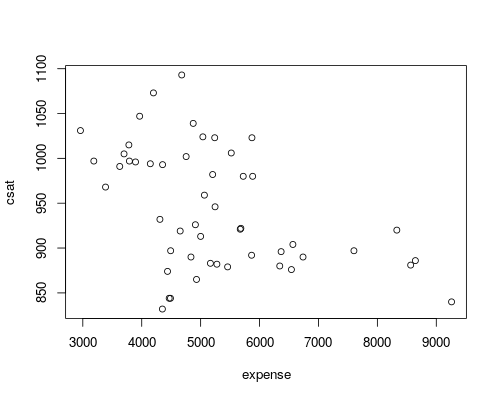
\includegraphics{R/Rmodels/images/statesCorr1.png}
\caption{}
\end{figure}

\section{Regression with continuous
outcomes}\label{regression-with-continuous-outcomes}

\begin{itemize}
\tightlist
\item
  Ordinary least squares (OLS) regression models can be fit with the
  \texttt{lm()} function
\item
  For example, we can use \texttt{lm} to predict SAT scores based on
  per-pupal expenditures:
\end{itemize}

\begin{Shaded}
\begin{Highlighting}[]
  \CommentTok{# Fit our regression model}
\NormalTok{  sat.mod <-}\StringTok{ }\KeywordTok{lm}\NormalTok{(csat }\OperatorTok{~}\StringTok{ }\NormalTok{expense, }\CommentTok{# regression formula}
                \DataTypeTok{data=}\NormalTok{states.data) }\CommentTok{# data }
                
  \CommentTok{# Summarize and print the results}
  \KeywordTok{summary}\NormalTok{(sat.mod) }\CommentTok{# show regression coefficients table}
\end{Highlighting}
\end{Shaded}

\subsection{\texorpdfstring{Why is the association between expense and
SAT scores
\emph{negative}?}{Why is the association between expense and SAT scores negative?}}\label{why-is-the-association-between-expense-and-sat-scores-negative}

Many people find it surprising that the per-capita expenditure on
students is negatively related to SAT scores. The beauty of multiple
regression is that we can try to pull these apart. What would the
association between expense and SAT scores be if there were no
difference among the states in the percentage of students taking the
SAT?

\begin{Shaded}
\begin{Highlighting}[]
  \KeywordTok{summary}\NormalTok{(}\KeywordTok{lm}\NormalTok{(csat }\OperatorTok{~}\StringTok{ }\NormalTok{expense }\OperatorTok{+}\StringTok{ }\NormalTok{percent, }\DataTypeTok{data =}\NormalTok{ states.data))}
\end{Highlighting}
\end{Shaded}

\subsection{\texorpdfstring{The \texttt{lm} class and
methods}{The lm class and methods}}\label{the-lm-class-and-methods}

OK, we fit our model. Now what?

\begin{itemize}
\tightlist
\item
  Examine the model object:
\end{itemize}

\begin{Shaded}
\begin{Highlighting}[]
  \KeywordTok{class}\NormalTok{(sat.mod)}
  \KeywordTok{str}\NormalTok{(sat.mod)}
  \KeywordTok{names}\NormalTok{(sat.mod)}
  \KeywordTok{methods}\NormalTok{(}\DataTypeTok{class =} \KeywordTok{class}\NormalTok{(sat.mod))}
\end{Highlighting}
\end{Shaded}

\begin{itemize}
\tightlist
\item
  Use function methods to get more information about the fit
\end{itemize}

\begin{Shaded}
\begin{Highlighting}[]
  \KeywordTok{summary}\NormalTok{(sat.mod)}
  \KeywordTok{coef}\NormalTok{(}\KeywordTok{summary}\NormalTok{(sat.mod))}
  \KeywordTok{methods}\NormalTok{(}\StringTok{"summary"}\NormalTok{)}
  \KeywordTok{confint}\NormalTok{(sat.mod)}
\end{Highlighting}
\end{Shaded}

\subsection{OLS regression
assumptions}\label{ols-regression-assumptions}

\begin{itemize}
\tightlist
\item
  OLS regression relies on several assumptions, including that the
  residuals are normally distributed and homoscedastic, the errors are
  independent and the relationships are linear.
\item
  Investigate these assumptions visually by plotting your model:
\end{itemize}

\begin{Shaded}
\begin{Highlighting}[]
  \KeywordTok{par}\NormalTok{(}\DataTypeTok{mfrow =} \KeywordTok{c}\NormalTok{(}\DecValTok{2}\NormalTok{, }\DecValTok{2}\NormalTok{)) }
  \KeywordTok{plot}\NormalTok{(sat.mod)}
\end{Highlighting}
\end{Shaded}

\subsection{Comparing models}\label{comparing-models}

Do congressional voting patterns predict SAT scores over and above
expense? Fit two models and compare them:

\begin{Shaded}
\begin{Highlighting}[]
  \CommentTok{# fit another model, adding house and senate as predictors}
\NormalTok{  sat.voting.mod <-}\StringTok{  }\KeywordTok{lm}\NormalTok{(csat }\OperatorTok{~}\StringTok{ }\NormalTok{expense }\OperatorTok{+}\StringTok{ }\NormalTok{house }\OperatorTok{+}\StringTok{ }\NormalTok{senate,}
                        \DataTypeTok{data =} \KeywordTok{na.omit}\NormalTok{(states.data))}
\NormalTok{  sat.mod <-}\StringTok{ }\KeywordTok{update}\NormalTok{(sat.mod, }\DataTypeTok{data=}\KeywordTok{na.omit}\NormalTok{(states.data))}

  \CommentTok{# compare using the anova() function}
  \KeywordTok{anova}\NormalTok{(sat.mod, sat.voting.mod)}
  \KeywordTok{coef}\NormalTok{(}\KeywordTok{summary}\NormalTok{(sat.voting.mod))}
\end{Highlighting}
\end{Shaded}

\section{Exercise 0}\label{exercise-0-1}

\textbf{Ordinary least squares regression}

Use the \emph{states.rds} data set. Fit a model predicting energy
consumed per capita (energy) from the percentage of residents living in
metropolitan areas (metro). Be sure to

\begin{enumerate}
\def\labelenumi{\arabic{enumi}.}
\tightlist
\item
  Examine/plot the data before fitting the model
\item
  Print and interpret the model \texttt{summary}
\item
  \texttt{plot} the model to look for deviations from modeling
  assumptions
\end{enumerate}

Select one or more additional predictors to add to your model and repeat
steps 1-3. Is this model significantly better than the model with
\emph{metro} as the only predictor?

\section{Interactions and factors}\label{interactions-and-factors}

\subsection{Modeling interactions}\label{modeling-interactions}

Interactions allow us assess the extent to which the association between
one predictor and the outcome depends on a second predictor. For
example: Does the association between expense and SAT scores depend on
the median income in the state?

\begin{Shaded}
\begin{Highlighting}[]
    \CommentTok{# Add the interaction to the model}
\NormalTok{  sat.expense.by.percent <-}\StringTok{ }\KeywordTok{lm}\NormalTok{(csat }\OperatorTok{~}\StringTok{ }\NormalTok{expense }\OperatorTok{+}\StringTok{ }\NormalTok{income }\OperatorTok{+}\StringTok{ }\NormalTok{expense }\OperatorTok{:}\StringTok{ }\NormalTok{income, }\DataTypeTok{data=}\NormalTok{states.data)}
\NormalTok{  sat.expense.by.percent <-}\StringTok{ }\KeywordTok{lm}\NormalTok{(csat }\OperatorTok{~}\StringTok{ }\NormalTok{expense }\OperatorTok{*}\StringTok{ }\NormalTok{income, }\DataTypeTok{data=}\NormalTok{states.data) }
  \CommentTok{# Show the results}
    \KeywordTok{coef}\NormalTok{(}\KeywordTok{summary}\NormalTok{(sat.expense.by.percent)) }\CommentTok{# show regression coefficients table}
\end{Highlighting}
\end{Shaded}

\subsection{Regression with categorical
predictors}\label{regression-with-categorical-predictors}

Let's try to predict SAT scores from region, a categorical variable.
Note that you must make sure R does not think your categorical variable
is numeric.

\begin{Shaded}
\begin{Highlighting}[]
  \CommentTok{# make sure R knows region is categorical}
  \KeywordTok{str}\NormalTok{(states.data}\OperatorTok{$}\NormalTok{region)}
\NormalTok{  states.data}\OperatorTok{$}\NormalTok{region <-}\StringTok{ }\KeywordTok{factor}\NormalTok{(states.data}\OperatorTok{$}\NormalTok{region)}

  \CommentTok{# Add region to the model}
\NormalTok{  sat.region <-}\StringTok{ }\KeywordTok{lm}\NormalTok{(csat }\OperatorTok{~}\StringTok{ }\NormalTok{region, }\DataTypeTok{data=}\NormalTok{states.data) }

  \CommentTok{# Show the results}
  \KeywordTok{coef}\NormalTok{(}\KeywordTok{summary}\NormalTok{(sat.region)) }\CommentTok{# show regression coefficients table}
  \KeywordTok{anova}\NormalTok{(sat.region) }\CommentTok{# show ANOVA table}
\end{Highlighting}
\end{Shaded}

Again, \textbf{make sure to tell R which variables are categorical by
converting them to factors!}

\subsection{Setting factor reference groups and
contrasts}\label{setting-factor-reference-groups-and-contrasts}

In the previous example we use the default contrasts for region. The
default in R is treatment contrasts, with the first level as the
reference. We can change the reference group or use another coding
scheme using the \texttt{C} function.

\begin{Shaded}
\begin{Highlighting}[]
  \CommentTok{# print default contrasts}
  \KeywordTok{contrasts}\NormalTok{(states.data}\OperatorTok{$}\NormalTok{region)}

  \CommentTok{# change the reference group}
\NormalTok{  states.data}\OperatorTok{$}\NormalTok{region <-}\StringTok{ }\KeywordTok{relevel}\NormalTok{(states.data}\OperatorTok{$}\NormalTok{region, }\DataTypeTok{ref =} \StringTok{"Midwest"}\NormalTok{)}
\NormalTok{  m1 <-}\StringTok{ }\KeywordTok{lm}\NormalTok{(csat }\OperatorTok{~}\StringTok{ }\NormalTok{region, }\DataTypeTok{data=}\NormalTok{states.data)}
  \KeywordTok{coef}\NormalTok{(}\KeywordTok{summary}\NormalTok{(m1))}

  \CommentTok{# drop the intercept to get group means}
  \KeywordTok{coef}\NormalTok{(}\KeywordTok{summary}\NormalTok{(}\KeywordTok{lm}\NormalTok{(csat }\OperatorTok{~}\StringTok{ }\DecValTok{0} \OperatorTok{+}\StringTok{ }\NormalTok{region, }\DataTypeTok{data=}\NormalTok{states.data)))}

  \CommentTok{# get all pairwise contrasts between means}
  \CommentTok{# install.packages("emmeans")}
  \KeywordTok{library}\NormalTok{(emmeans)}
\NormalTok{  means <-}\StringTok{ }\KeywordTok{emmeans}\NormalTok{(m1, }\DataTypeTok{specs =} \OperatorTok{~}\StringTok{ }\NormalTok{region)}
  \KeywordTok{contrast}\NormalTok{(means, }\DataTypeTok{method =} \StringTok{"pairwise"}\NormalTok{)}

  \CommentTok{# change the coding scheme}
  \KeywordTok{coef}\NormalTok{(}\KeywordTok{summary}\NormalTok{(}\KeywordTok{lm}\NormalTok{(csat }\OperatorTok{~}\StringTok{ }\KeywordTok{C}\NormalTok{(region, contr.helmert), }\DataTypeTok{data=}\NormalTok{states.data)))}
\end{Highlighting}
\end{Shaded}

See also \texttt{?contrasts}, \texttt{?contr.treatment}, and
\texttt{?relevel}.

\section{Exercise 1}\label{exercise-1-1}

\textbf{Interactions and factors}

Use the states data set.

\begin{enumerate}
\def\labelenumi{\arabic{enumi}.}
\item
  Add on to the regression equation that you created in exercise 1 by
  generating an interaction term and testing the interaction.
\item
  Try adding region to the model. Are there significant differences
  across the four regions?
\end{enumerate}

\section{Regression with binary
outcomes}\label{regression-with-binary-outcomes}

\subsection{Logistic regression}\label{logistic-regression}

This far we have used the \texttt{lm} function to fit our regression
models. \texttt{lm} is great, but limited--in particular it only fits
models for continuous dependent variables. For categorical dependent
variables we can use the \texttt{glm()} function.

For these models we will use a different dataset, drawn from the
National Health Interview Survey. From the
\href{http://www.cdc.gov/nchs/nhis.htm}{CDC website}:

\begin{quote}
The National Health Interview Survey (NHIS) has monitored the health of
the nation since 1957. NHIS data on a broad range of health topics are
collected through personal household interviews. For over 50 years, the
U.S. Census Bureau has been the data collection agent for the National
Health Interview Survey. Survey results have been instrumental in
providing data to track health status, health care access, and progress
toward achieving national health objectives.
\end{quote}

Load the National Health Interview Survey data:

\begin{Shaded}
\begin{Highlighting}[]
\NormalTok{  NH11 <-}\StringTok{ }\KeywordTok{read_rds}\NormalTok{(}\StringTok{"dataSets/NatHealth2011.rds"}\NormalTok{)}
\end{Highlighting}
\end{Shaded}

\subsection{Logistic regression
example}\label{logistic-regression-example}

Let's predict the probability of being diagnosed with hypertension based
on age, sex, sleep, and bmi

\begin{Shaded}
\begin{Highlighting}[]
  \KeywordTok{str}\NormalTok{(NH11}\OperatorTok{$}\NormalTok{hypev) }\CommentTok{# check stucture of hypev}
  \KeywordTok{levels}\NormalTok{(NH11}\OperatorTok{$}\NormalTok{hypev) }\CommentTok{# check levels of hypev}
  \CommentTok{# collapse all missing values to NA}
\NormalTok{  NH11}\OperatorTok{$}\NormalTok{hypev <-}\StringTok{ }\KeywordTok{factor}\NormalTok{(NH11}\OperatorTok{$}\NormalTok{hypev, }\DataTypeTok{levels=}\KeywordTok{c}\NormalTok{(}\StringTok{"2 No"}\NormalTok{, }\StringTok{"1 Yes"}\NormalTok{))}
  \CommentTok{# run our regression model}
\NormalTok{  hyp.out <-}\StringTok{ }\KeywordTok{glm}\NormalTok{(hypev }\OperatorTok{~}\StringTok{ }\NormalTok{age_p }\OperatorTok{+}\StringTok{ }\NormalTok{sex }\OperatorTok{+}\StringTok{ }\NormalTok{sleep }\OperatorTok{+}\StringTok{ }\NormalTok{bmi,}
                \DataTypeTok{data =}\NormalTok{ NH11, }\DataTypeTok{family =} \KeywordTok{binomial}\NormalTok{(}\DataTypeTok{link =} \StringTok{"logit"}\NormalTok{))}
  \KeywordTok{coef}\NormalTok{(}\KeywordTok{summary}\NormalTok{(hyp.out))}
\end{Highlighting}
\end{Shaded}

\subsection{Logistic regression
coefficients}\label{logistic-regression-coefficients}

Generalized linear models use link functions, so raw coefficients are
difficult to interpret. For example, the age coefficient of .06 in the
previous model tells us that for every one unit increase in age, the log
odds of hypertension diagnosis increases by 0.06. Since most of us are
not used to thinking in log odds this is not too helpful!

One solution is to transform the coefficients to make them easier to
interpret

\begin{Shaded}
\begin{Highlighting}[]
\NormalTok{  hyp.out.tab <-}\StringTok{ }\KeywordTok{coef}\NormalTok{(}\KeywordTok{summary}\NormalTok{(hyp.out))}
\NormalTok{  hyp.out.tab[, }\StringTok{"Estimate"}\NormalTok{] <-}\StringTok{ }\KeywordTok{exp}\NormalTok{(}\KeywordTok{coef}\NormalTok{(hyp.out))}
\NormalTok{  hyp.out.tab}
\end{Highlighting}
\end{Shaded}

\subsection{Packages for computing and graphing predicted
values}\label{packages-for-computing-and-graphing-predicted-values}

Instead of doing all this ourselves, we can use the effects package to
compute quantities of interest for us.

\begin{Shaded}
\begin{Highlighting}[]
  \KeywordTok{library}\NormalTok{(effects)}
\NormalTok{  eff <-}\StringTok{ }\KeywordTok{allEffects}\NormalTok{(hyp.out)}
\NormalTok{  eff2 <-}\StringTok{ }\KeywordTok{allEffects}\NormalTok{(hyp.out, }\DataTypeTok{xlevels =} \KeywordTok{list}\NormalTok{(age_p, }\KeywordTok{seq}\NormalTok{(}\DecValTok{20}\NormalTok{, }\DecValTok{80}\NormalTok{, }\DataTypeTok{by =} \DecValTok{5}\NormalTok{)))}
  \KeywordTok{plot}\NormalTok{(eff)}
  \KeywordTok{as.data.frame}\NormalTok{(eff) }\CommentTok{# confidence intervals}
\end{Highlighting}
\end{Shaded}

\begin{figure}
\centering
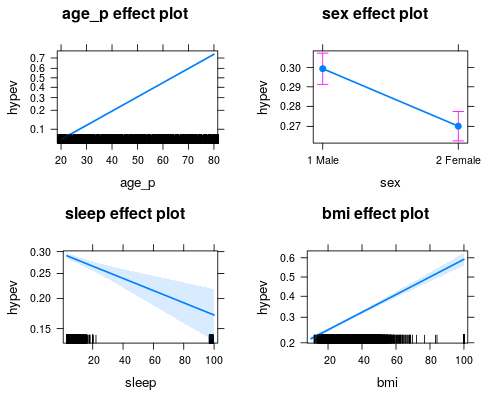
\includegraphics{R/Rmodels/images/effects1.png}
\caption{}
\end{figure}

\section{Exercise 2}\label{exercise-2-1}

\textbf{Logistic regression}

Use the NH11 data set that we loaded earlier.

\begin{enumerate}
\def\labelenumi{\arabic{enumi}.}
\tightlist
\item
  Use glm to conduct a logistic regression to predict ever worked
  (everwrk) using age (age\_p) and marital status (r\_maritl).
\item
  Predict the probability of working for each level of marital status.
\end{enumerate}

Note that the data is not perfectly clean and ready to be modeled. You
will need to clean up at least some of the variables before fitting the
model.

\section{Multilevel modeling}\label{multilevel-modeling}

\subsection{Multilevel modeling
overview}\label{multilevel-modeling-overview}

\begin{itemize}
\tightlist
\item
  Multi-level (AKA hierarchical) models are a type of mixed-effects
  models
\item
  Used to model variation due to group membership where the goal is to
  generalize to a population of groups
\item
  Can model different intercepts and/or slopes for each group
\item
  Mixed-effecs models include two types of predictors: fixed-effects and
  random effects
\item
  Fixed-effects -- observed levels are of direct interest (.e.g, sex,
  political party\ldots{})
\item
  Random-effects -- observed levels not of direct interest: goal is to
  make inferences to a population represented by observed levels
\item
  In R the lme4 package is the most popular for mixed effects models
\item
  Use the \texttt{lmer} function for liner mixed models, \texttt{glmer}
  for generalized mixed models
\end{itemize}

\begin{Shaded}
\begin{Highlighting}[]
  \KeywordTok{library}\NormalTok{(lme4)}
\end{Highlighting}
\end{Shaded}

\subsection{The Exam data}\label{the-exam-data}

The Exam data set contans exam scores of 4,059 students from 65 schools
in Inner London. The variable names are as follows:

\begin{longtable}[]{@{}ll@{}}
\toprule
variable & Description\tabularnewline
\midrule
\endhead
school & School ID - a factor.\tabularnewline
normexam & Normalized exam score.\tabularnewline
standLRT & Standardised LR test score.\tabularnewline
student & Student id (within school) - a factor\tabularnewline
\bottomrule
\end{longtable}

\begin{Shaded}
\begin{Highlighting}[]
\NormalTok{  Exam <-}\StringTok{ }\KeywordTok{read_rds}\NormalTok{(}\StringTok{"dataSets/Exam.rds"}\NormalTok{)}
\end{Highlighting}
\end{Shaded}

\subsection{The null model and ICC}\label{the-null-model-and-icc}

As a preliminary step it is often useful to partition the variance in
the dependent variable into the various levels. This can be accomplished
by running a null model (i.e., a model with a random effects grouping
structure, but no fixed-effects predictors).

\begin{Shaded}
\begin{Highlighting}[]
  \CommentTok{# null model, grouping by school but not fixed effects.}
\NormalTok{  Norm1 <-}\KeywordTok{lmer}\NormalTok{(normexam }\OperatorTok{~}\StringTok{ }\DecValTok{1} \OperatorTok{+}\StringTok{ }\NormalTok{(}\DecValTok{1}\OperatorTok{|}\NormalTok{school),}
                \DataTypeTok{data=}\KeywordTok{na.omit}\NormalTok{(Exam), }\DataTypeTok{REML =} \OtherTok{FALSE}\NormalTok{)}
  \KeywordTok{summary}\NormalTok{(Norm1)}
\end{Highlighting}
\end{Shaded}

The is .169/(.169 + .848) = .17: 17\% of the variance is at the school
level.

There is no consensus on how to calculate p-values for MLMs; hence why
they are omitted from the \texttt{lme4} output. But, we can calculate
approximate p-values using the \texttt{lmerTest} package.

\subsection{Adding fixed-effects
predictors}\label{adding-fixed-effects-predictors}

Predict exam scores from student's standardized tests scores

\begin{Shaded}
\begin{Highlighting}[]
\NormalTok{  Norm2 <-}\KeywordTok{lmer}\NormalTok{(normexam }\OperatorTok{~}\StringTok{ }\DecValTok{1} \OperatorTok{+}\StringTok{ }\NormalTok{standLRT }\OperatorTok{+}\StringTok{ }\NormalTok{(}\DecValTok{1} \OperatorTok{|}\StringTok{ }\NormalTok{school),}
               \DataTypeTok{data=}\KeywordTok{na.omit}\NormalTok{(Exam), }\DataTypeTok{REML =} \OtherTok{FALSE}\NormalTok{) }
  \KeywordTok{summary}\NormalTok{(Norm2) }
\end{Highlighting}
\end{Shaded}

\subsection{Multiple degree of freedom
comparisons}\label{multiple-degree-of-freedom-comparisons}

As with \texttt{lm} and \texttt{glm} models, you can compare the two
\texttt{lmer} models using the \texttt{anova} function.

\begin{Shaded}
\begin{Highlighting}[]
  \KeywordTok{anova}\NormalTok{(Norm1, Norm2)}
\end{Highlighting}
\end{Shaded}

\subsection{Random slopes}\label{random-slopes}

Add a random effect of students' standardized test scores as well. Now
in addition to estimating the distribution of intercepts across schools,
we also estimate the distribution of the slope of exam on standardized
test.

\begin{Shaded}
\begin{Highlighting}[]
\NormalTok{  Norm3 <-}\StringTok{ }\KeywordTok{lmer}\NormalTok{(normexam }\OperatorTok{~}\StringTok{ }\DecValTok{1} \OperatorTok{+}\StringTok{ }\NormalTok{standLRT }\OperatorTok{+}\StringTok{ }\NormalTok{(}\DecValTok{1} \OperatorTok{+}\StringTok{ }\NormalTok{standLRT }\OperatorTok{|}\StringTok{ }\NormalTok{school), }
                \DataTypeTok{data =} \KeywordTok{na.omit}\NormalTok{(Exam), }\DataTypeTok{REML =} \OtherTok{FALSE}\NormalTok{) }
  \KeywordTok{summary}\NormalTok{(Norm3) }
\end{Highlighting}
\end{Shaded}

\subsection{Test the significance of the random
slope}\label{test-the-significance-of-the-random-slope}

To test the significance of a random slope just compare models with and
without the random slope term

\begin{Shaded}
\begin{Highlighting}[]
  \KeywordTok{anova}\NormalTok{(Norm2, Norm3) }
\end{Highlighting}
\end{Shaded}

\section{Exercise 3}\label{exercise-3-1}

\textbf{Multilevel modeling}

Use the dataset, bh1996:

\begin{Shaded}
\begin{Highlighting}[]
\KeywordTok{data}\NormalTok{(bh1996, }\DataTypeTok{package=}\StringTok{"multilevel"}\NormalTok{)}
\end{Highlighting}
\end{Shaded}

From the data documentation:

\begin{quote}
Variables are Leadership Climate (LEAD), Well-Being (WBEING), Work Hours
(HRS), and cluster group (GRP).
\end{quote}

\begin{enumerate}
\def\labelenumi{\arabic{enumi}.}
\tightlist
\item
  Create a null model predicting wellbeing (``WBEING'')
\item
  Calculate the ICC for your null model
\item
  Run a second multi-level model that adds two individual-level
  predictors, average number of hours worked (``HRS'') and leadership
  skills (``LEAD'') to the model and interpret your output.
\item
  Now, add a random effect of average number of hours worked (``HRS'')
  to the model and interpret your output. Test the significance of this
  random term.
\end{enumerate}

\section{Exercise solutions}\label{exercise-solutions-1}

\subsection{Ex 0: prototype}\label{ex-0-prototype-1}

Use the \emph{states.rds} data set.

\begin{Shaded}
\begin{Highlighting}[]
\NormalTok{  states <-}\StringTok{ }\KeywordTok{read_rds}\NormalTok{(}\StringTok{"dataSets/states.rds"}\NormalTok{)}
\end{Highlighting}
\end{Shaded}

Fit a model predicting energy consumed per capita (energy) from the
percentage of residents living in metropolitan areas (metro). Be sure to

\begin{enumerate}
\def\labelenumi{\arabic{enumi}.}
\tightlist
\item
  Examine/plot the data before fitting the model
\end{enumerate}

\begin{Shaded}
\begin{Highlighting}[]
\NormalTok{  states.en.met <-}\StringTok{ }\KeywordTok{subset}\NormalTok{(states, }\DataTypeTok{select =} \KeywordTok{c}\NormalTok{(}\StringTok{"metro"}\NormalTok{, }\StringTok{"energy"}\NormalTok{))}
  \KeywordTok{summary}\NormalTok{(states.en.met)}
  \KeywordTok{plot}\NormalTok{(states.en.met)}
  \KeywordTok{cor}\NormalTok{(states.en.met, }\DataTypeTok{use=}\StringTok{"pairwise"}\NormalTok{)}
\end{Highlighting}
\end{Shaded}

\begin{enumerate}
\def\labelenumi{\arabic{enumi}.}
\setcounter{enumi}{1}
\tightlist
\item
  Print and interpret the model \texttt{summary}
\end{enumerate}

\begin{Shaded}
\begin{Highlighting}[]
\NormalTok{  mod.en.met <-}\StringTok{ }\KeywordTok{lm}\NormalTok{(energy }\OperatorTok{~}\StringTok{ }\NormalTok{metro, }\DataTypeTok{data =}\NormalTok{ states)}
  \KeywordTok{summary}\NormalTok{(mod.en.met)}
\end{Highlighting}
\end{Shaded}

\begin{enumerate}
\def\labelenumi{\arabic{enumi}.}
\setcounter{enumi}{2}
\tightlist
\item
  \texttt{plot} the model to look for deviations from modeling
  assumptions
\end{enumerate}

\begin{Shaded}
\begin{Highlighting}[]
  \KeywordTok{plot}\NormalTok{(mod.en.met)}
\end{Highlighting}
\end{Shaded}

Select one or more additional predictors to add to your model and repeat
steps 1-3. Is this model significantly better than the model with
\emph{metro} as the only predictor?

\begin{Shaded}
\begin{Highlighting}[]
\NormalTok{  states.en.met.pop.wst <-}\StringTok{ }\KeywordTok{subset}\NormalTok{(states, }\DataTypeTok{select =} \KeywordTok{c}\NormalTok{(}\StringTok{"energy"}\NormalTok{, }\StringTok{"metro"}\NormalTok{, }\StringTok{"pop"}\NormalTok{, }\StringTok{"waste"}\NormalTok{))}
  \KeywordTok{summary}\NormalTok{(states.en.met.pop.wst)}
  \KeywordTok{plot}\NormalTok{(states.en.met.pop.wst)}
  \KeywordTok{cor}\NormalTok{(states.en.met.pop.wst, }\DataTypeTok{use =} \StringTok{"pairwise"}\NormalTok{)}
\NormalTok{  mod.en.met.pop.waste <-}\StringTok{ }\KeywordTok{lm}\NormalTok{(energy }\OperatorTok{~}\StringTok{ }\NormalTok{metro }\OperatorTok{+}\StringTok{ }\NormalTok{pop }\OperatorTok{+}\StringTok{ }\NormalTok{waste, }\DataTypeTok{data =}\NormalTok{ states)}
  \KeywordTok{summary}\NormalTok{(mod.en.met.pop.waste)}
  \KeywordTok{anova}\NormalTok{(mod.en.met, mod.en.met.pop.waste)}
\end{Highlighting}
\end{Shaded}

\subsection{Ex 1: prototype}\label{ex-1-prototype-1}

Use the states data set.

\begin{enumerate}
\def\labelenumi{\arabic{enumi}.}
\tightlist
\item
  Add on to the regression equation that you created in exercise 1 by
  generating an interaction term and testing the interaction.
\end{enumerate}

\begin{Shaded}
\begin{Highlighting}[]
\NormalTok{  mod.en.metro.by.waste <-}\StringTok{ }\KeywordTok{lm}\NormalTok{(energy }\OperatorTok{~}\StringTok{ }\NormalTok{metro }\OperatorTok{*}\StringTok{ }\NormalTok{waste, }\DataTypeTok{data =}\NormalTok{ states)}
\end{Highlighting}
\end{Shaded}

\begin{enumerate}
\def\labelenumi{\arabic{enumi}.}
\setcounter{enumi}{1}
\tightlist
\item
  Try adding a region to the model. Are there significant differences
  across the four regions?
\end{enumerate}

\begin{Shaded}
\begin{Highlighting}[]
\NormalTok{  mod.en.region <-}\StringTok{ }\KeywordTok{lm}\NormalTok{(energy }\OperatorTok{~}\StringTok{ }\NormalTok{metro }\OperatorTok{*}\StringTok{ }\NormalTok{waste }\OperatorTok{+}\StringTok{ }\NormalTok{region, }\DataTypeTok{data =}\NormalTok{ states)}
  \KeywordTok{anova}\NormalTok{(mod.en.region)}
\end{Highlighting}
\end{Shaded}

\subsection{Ex 2: prototype}\label{ex-2-prototype-1}

Use the NH11 data set that we loaded earlier. Note that the data is not
perfectly clean and ready to be modeled. You will need to clean up at
least some of the variables before fitting the model.

\begin{enumerate}
\def\labelenumi{\arabic{enumi}.}
\tightlist
\item
  Use glm to conduct a logistic regression to predict ever worked
  (everwrk) using age (age\_p) and marital status (r\_maritl).
\end{enumerate}

\begin{Shaded}
\begin{Highlighting}[]
\NormalTok{  nh11.wrk.age.mar <-}\StringTok{ }\KeywordTok{subset}\NormalTok{(NH11, }\DataTypeTok{select =} \KeywordTok{c}\NormalTok{(}\StringTok{"everwrk"}\NormalTok{, }\StringTok{"age_p"}\NormalTok{, }\StringTok{"r_maritl"}\NormalTok{))}
  \KeywordTok{summary}\NormalTok{(nh11.wrk.age.mar)}

\NormalTok{  NH11 <-}\StringTok{ }\KeywordTok{transform}\NormalTok{(NH11,}
                    \DataTypeTok{everwrk =} \KeywordTok{factor}\NormalTok{(everwrk, }\DataTypeTok{levels =} \KeywordTok{c}\NormalTok{(}\StringTok{"1 Yes"}\NormalTok{, }\StringTok{"2 No"}\NormalTok{)),}
                    \DataTypeTok{r_maritl =} \KeywordTok{droplevels}\NormalTok{(r_maritl))}

\NormalTok{  mod.wk.age.mar <-}\StringTok{ }\KeywordTok{glm}\NormalTok{(everwrk }\OperatorTok{~}\StringTok{ }\NormalTok{age_p }\OperatorTok{+}\StringTok{ }\NormalTok{r_maritl, }\DataTypeTok{data =}\NormalTok{ NH11,}
                        \DataTypeTok{family =} \KeywordTok{binomial}\NormalTok{(}\DataTypeTok{link =} \StringTok{"logit"}\NormalTok{))}

  \KeywordTok{summary}\NormalTok{(mod.wk.age.mar)}
\end{Highlighting}
\end{Shaded}

\begin{enumerate}
\def\labelenumi{\arabic{enumi}.}
\setcounter{enumi}{1}
\tightlist
\item
  Predict the probability of working for each level of marital status.
\end{enumerate}

\begin{Shaded}
\begin{Highlighting}[]
  \KeywordTok{library}\NormalTok{(effects)}
  \KeywordTok{data.frame}\NormalTok{(}\KeywordTok{Effect}\NormalTok{(}\StringTok{"r_maritl"}\NormalTok{, mod.wk.age.mar))}
\end{Highlighting}
\end{Shaded}

\subsection{Ex 3: prototype}\label{ex-3-prototype-1}

Use the dataset, bh1996:

\begin{Shaded}
\begin{Highlighting}[]
  \KeywordTok{data}\NormalTok{(bh1996, }\DataTypeTok{package=}\StringTok{"multilevel"}\NormalTok{)}
\end{Highlighting}
\end{Shaded}

From the data documentation:

\begin{quote}
Variables are Cohesion (COHES), Leadership Climate (LEAD), Well-Being
(WBEING) and Work Hours (HRS). Each of these variables has two variants
- a group mean version that replicates each group mean for every
individual, and a within-group version where the group mean is
subtracted from each individual response. The group mean version is
designated with a G. (e.g., G.HRS), and the within-group version is
designated with a W. (e.g., W.HRS).
\end{quote}

Note that the group identifier is named ``GRP''.

\begin{enumerate}
\def\labelenumi{\arabic{enumi}.}
\tightlist
\item
  Create a null model predicting wellbeing (``WBEING'')
\end{enumerate}

\begin{Shaded}
\begin{Highlighting}[]
  \KeywordTok{library}\NormalTok{(lme4)}
\NormalTok{  mod.grp0 <-}\StringTok{ }\KeywordTok{lmer}\NormalTok{(WBEING }\OperatorTok{~}\StringTok{ }\DecValTok{1} \OperatorTok{+}\StringTok{ }\NormalTok{(}\DecValTok{1} \OperatorTok{|}\StringTok{ }\NormalTok{GRP), }\DataTypeTok{data =}\NormalTok{ bh1996)}
  \KeywordTok{summary}\NormalTok{(mod.grp0)}
\end{Highlighting}
\end{Shaded}

\begin{enumerate}
\def\labelenumi{\arabic{enumi}.}
\setcounter{enumi}{2}
\tightlist
\item
  Run a second multi-level model that adds two individual-level
  predictors, average number of hours worked (``HRS'') and leadership
  skills (``LEAD'') to the model and interpret your output.
\end{enumerate}

\begin{Shaded}
\begin{Highlighting}[]
\NormalTok{  mod.grp1 <-}\StringTok{ }\KeywordTok{lmer}\NormalTok{(WBEING }\OperatorTok{~}\StringTok{ }\NormalTok{HRS }\OperatorTok{+}\StringTok{ }\NormalTok{LEAD }\OperatorTok{+}\StringTok{ }\NormalTok{(}\DecValTok{1} \OperatorTok{|}\StringTok{ }\NormalTok{GRP), }\DataTypeTok{data =}\NormalTok{ bh1996)}
  \KeywordTok{summary}\NormalTok{(mod.grp1)}
\end{Highlighting}
\end{Shaded}

\begin{enumerate}
\def\labelenumi{\arabic{enumi}.}
\setcounter{enumi}{2}
\tightlist
\item
  Now, add a random effect of average number of hours worked (``HRS'')
  to the model and interpret your output. Test the significance of this
  random term.
\end{enumerate}

\begin{Shaded}
\begin{Highlighting}[]
\NormalTok{  mod.grp2 <-}\StringTok{ }\KeywordTok{lmer}\NormalTok{(WBEING }\OperatorTok{~}\StringTok{ }\NormalTok{HRS }\OperatorTok{+}\StringTok{ }\NormalTok{LEAD }\OperatorTok{+}\StringTok{ }\NormalTok{(}\DecValTok{1} \OperatorTok{+}\StringTok{ }\NormalTok{HRS }\OperatorTok{|}\StringTok{ }\NormalTok{GRP), }\DataTypeTok{data =}\NormalTok{ bh1996)}
  \KeywordTok{anova}\NormalTok{(mod.grp1, mod.grp2)}
\end{Highlighting}
\end{Shaded}

\section{Wrap-up}\label{wrap-up-1}

\subsection{Feedback}\label{feedback-1}

These workshops are a work in progress, please provide any feedback to:
\href{mailto:help@iq.harvard.edu}{\nolinkurl{help@iq.harvard.edu}}

\subsection{Resources}\label{resources-1}

\begin{itemize}
\tightlist
\item
  IQSS

  \begin{itemize}
  \tightlist
  \item
    \href{https://dss.iq.harvard.edu/workshop-materials}{Workshops}
  \item
    \href{https://dss.iq.harvard.edu/}{Data Science Services}
  \item
    \href{https://iqss.github.io/dss-rce/}{Research Computing
    Environment}
  \end{itemize}
\end{itemize}

\chapter{R Graphics}\label{r-graphics}

\textbf{Topics}

\begin{itemize}
\tightlist
\item
  R ggplot2 package
\item
  Setup basic plots
\item
  Add and modify scales and legends
\item
  Manipulate plot labels
\item
  Change and create plot themes
\end{itemize}

\section{Setup}\label{setup-2}

\subsection{Software \& materials}\label{software-materials-2}

You should have R and RStudio installed --- if not:

\begin{itemize}
\tightlist
\item
  Download and install \href{http://cran.r-project.org}{R}
\item
  Download and install
  \href{https://www.rstudio.com/products/rstudio/download/\#download}{RStudio}
\end{itemize}

Download materials:

\begin{itemize}
\tightlist
\item
  \href{http://tutorials.iq.harvard.edu/R/Rgraphics.zip}{Download
  workshop materials}
\item
  Extract materials from \texttt{Rgraphics.zip} and move to your
  desktop.
\end{itemize}

Start RStudio and create a new project:

\begin{itemize}
\tightlist
\item
  On Windows click the start button and search for RStudio. On Mac
  RStudio will be in your applications folder.
\item
  In Rstudio go to \texttt{File\ -\textgreater{}\ New\ Project}.
\item
  Choose \texttt{Existing\ Directory} and browse to the
  \texttt{Rgraphics} directory.
\item
  Choose \texttt{File\ -\textgreater{}\ Open\ File} and select the blank
  version of the \texttt{.Rmd} file.
\end{itemize}

Install the \href{https://www.tidyverse.org/}{tidyverse} suite of
packages:

\begin{Shaded}
\begin{Highlighting}[]
\CommentTok{# install.packages("tidyverse")}
\KeywordTok{library}\NormalTok{(tidyverse)}
\end{Highlighting}
\end{Shaded}

Set your working directory so you don't have to type the full path names
to your data and other files

\begin{Shaded}
\begin{Highlighting}[]
  \CommentTok{# set the working directory}
  \CommentTok{# setwd("~/Desktop/Rgraphics") # UNIX-based}
  \CommentTok{# setwd("C:/Users/dataclass/Desktop/Rgraphics") # MS Windows}
\end{Highlighting}
\end{Shaded}

\subsection{Goals}\label{goals-2}

Class Structure and Organization:

\begin{itemize}
\tightlist
\item
  Ask questions at any time. Really!
\item
  Collaboration is encouraged - please spend a minute introducing
  yourself to your neighbors!
\end{itemize}

This is an intermediate R course:

\begin{itemize}
\tightlist
\item
  Assumes working knowledge of R
\item
  Relatively fast-paced
\item
  Focus is on \texttt{ggplot2} graphics; other packages will not be
  covered
\end{itemize}

\subsection{Starting at the end}\label{starting-at-the-end}

By the end of the workshop you will be able to reproduce this graphic
from the Economist:

\begin{figure}
\centering
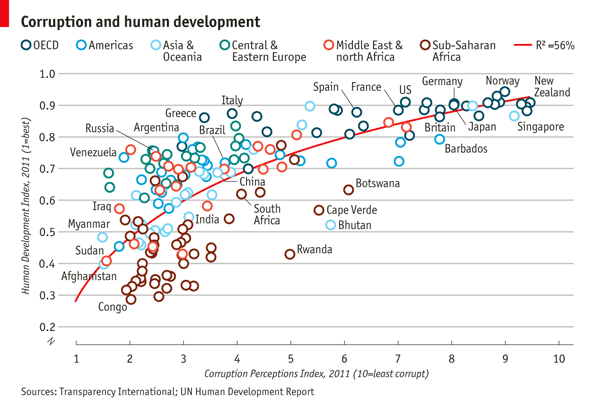
\includegraphics{R/Rgraphics/images/Economist1.png}
\caption{img}
\end{figure}

\section{\texorpdfstring{Why
\texttt{ggplot2}?}{Why ggplot2?}}\label{why-ggplot2}

Advantages of ggplot2

\begin{itemize}
\tightlist
\item
  consistent underlying \texttt{grammar\ of\ graphics} (Wilkinson, 2005)
\item
  plot specification at a high level of abstraction
\item
  very flexible
\item
  theme system for polishing plot appearance
\item
  mature and complete graphics system
\item
  many users, active mailing list
\end{itemize}

That said, there are some things you cannot (or should not) do With
ggplot2:

\begin{itemize}
\tightlist
\item
  3-dimensional graphics (see the rgl package)
\item
  Graph-theory type graphs (nodes/edges layout; see the igraph package)
\item
  Interactive graphics (see the ggvis package)
\end{itemize}

\subsection{What is the Grammar Of
Graphics?}\label{what-is-the-grammar-of-graphics}

The basic idea: independently specify plot building blocks and combine
them to create just about any kind of graphical display you want.
Building blocks of a graph include:

\begin{itemize}
\tightlist
\item
  data
\item
  aesthetic mapping
\item
  geometric object
\item
  statistical transformations
\item
  scales
\item
  coordinate system
\item
  position adjustments
\item
  faceting
\end{itemize}

\subsection{\texorpdfstring{Example data:
\texttt{housing\ prices}}{Example data: housing prices}}\label{example-data-housing-prices}

Let's look at housing prices.

\begin{Shaded}
\begin{Highlighting}[]
\NormalTok{housing <-}\StringTok{ }\KeywordTok{read_csv}\NormalTok{(}\StringTok{"dataSets/landdata-states.csv"}\NormalTok{)}
\KeywordTok{head}\NormalTok{(housing[}\DecValTok{1}\OperatorTok{:}\DecValTok{5}\NormalTok{])}
\end{Highlighting}
\end{Shaded}

\subsection{\texorpdfstring{\texttt{ggplot2} VS base
graphics}{ggplot2 VS base graphics}}\label{ggplot2-vs-base-graphics}

Compared to base graphics, \texttt{ggplot2}

\begin{itemize}
\tightlist
\item
  is more verbose for simple / canned graphics
\item
  is less verbose for complex / custom graphics
\item
  does not have methods (data should always be in a \texttt{data.frame})
\item
  uses a different system for adding plot elements
\end{itemize}

\subsection{For simple graphs}\label{for-simple-graphs}

Base graphics histogram example:

\begin{Shaded}
\begin{Highlighting}[]
\KeywordTok{hist}\NormalTok{(housing}\OperatorTok{$}\NormalTok{Home.Value)}
\end{Highlighting}
\end{Shaded}

\texttt{ggplot2} histogram example:

\begin{Shaded}
\begin{Highlighting}[]
\KeywordTok{library}\NormalTok{(ggplot2)}
\KeywordTok{ggplot}\NormalTok{(housing, }\KeywordTok{aes}\NormalTok{(}\DataTypeTok{x =}\NormalTok{ Home.Value)) }\OperatorTok{+}
\StringTok{  }\KeywordTok{geom_histogram}\NormalTok{()}
\end{Highlighting}
\end{Shaded}

\subsection{For more complex graphs:}\label{for-more-complex-graphs}

Base graphics colored scatter plot example:

\begin{Shaded}
\begin{Highlighting}[]
\KeywordTok{plot}\NormalTok{(Home.Value }\OperatorTok{~}\StringTok{ }\NormalTok{Date,}
     \DataTypeTok{col =} \KeywordTok{factor}\NormalTok{(State),}
     \DataTypeTok{data =} \KeywordTok{filter}\NormalTok{(housing, State }\OperatorTok\StringTok{ }\KeywordTok{c}\NormalTok{(}\StringTok{"MA"}\NormalTok{, }\StringTok{"TX"}\NormalTok{)))}
\KeywordTok{legend}\NormalTok{(}\StringTok{"topleft"}\NormalTok{,}
       \DataTypeTok{legend =} \KeywordTok{c}\NormalTok{(}\StringTok{"MA"}\NormalTok{, }\StringTok{"TX"}\NormalTok{),}
       \DataTypeTok{col =} \KeywordTok{c}\NormalTok{(}\StringTok{"black"}\NormalTok{, }\StringTok{"red"}\NormalTok{),}
       \DataTypeTok{pch =} \DecValTok{1}\NormalTok{)}
\end{Highlighting}
\end{Shaded}

\texttt{ggplot2} colored scatter plot example:

\begin{Shaded}
\begin{Highlighting}[]
\KeywordTok{ggplot}\NormalTok{(}\KeywordTok{filter}\NormalTok{(housing, State }\OperatorTok\StringTok{ }\KeywordTok{c}\NormalTok{(}\StringTok{"MA"}\NormalTok{, }\StringTok{"TX"}\NormalTok{)),}
       \KeywordTok{aes}\NormalTok{(}\DataTypeTok{x=}\NormalTok{Date,}
           \DataTypeTok{y=}\NormalTok{Home.Value,}
           \DataTypeTok{color=}\NormalTok{State))}\OperatorTok{+}
\StringTok{  }\KeywordTok{geom_point}\NormalTok{()}
\end{Highlighting}
\end{Shaded}

\texttt{ggplot2} wins!

\section{Geometric objects and
aesthetics}\label{geometric-objects-and-aesthetics}

\subsection{Aesthetic mapping}\label{aesthetic-mapping}

In ggplot land \emph{aesthetic} means ``something you can see''.
Examples include:

\begin{itemize}
\tightlist
\item
  position (i.e., on the x and y axes)
\item
  color (``outside'' color)
\item
  fill (``inside'' color)
\item
  shape (of points)
\item
  linetype
\item
  size
\end{itemize}

Each type of geom accepts only a subset of all aesthetics;refer to the
geom help pages to see what mappings each geom accepts. Aesthetic
mappings are set with the \texttt{aes()} function.

\subsection{\texorpdfstring{Geometic objects
(\texttt{geom})}{Geometic objects (geom)}}\label{geometic-objects-geom}

Geometric objects are the actual marks we put on a plot. Examples
include:

\begin{itemize}
\tightlist
\item
  points (\texttt{geom\_point}, for scatter plots, dot plots, etc.)
\item
  lines (\texttt{geom\_line}, for time series, trend lines, etc.)
\item
  boxplot (\texttt{geom\_boxplot}, for, well, boxplots!)
\end{itemize}

A plot must have at least one geom; there is no upper limit. You can add
a geom to a plot using the \texttt{+} operator

You can get a list of available geometric objects using the code below:

\begin{Shaded}
\begin{Highlighting}[]
\KeywordTok{help.search}\NormalTok{(}\StringTok{"geom_"}\NormalTok{, }\DataTypeTok{package =} \StringTok{"ggplot2"}\NormalTok{)}
\end{Highlighting}
\end{Shaded}

or simply type \texttt{geom\_\textless{}tab\textgreater{}} in any good R
IDE (such as Rstudio or ESS) to see a list of functions starting with
\texttt{geom\_}.

\subsection{Points (scatterplot)}\label{points-scatterplot}

Now that we know about geometric objects and aesthetic mapping, we can
make a ggplot. \texttt{geom\_point} requires mappings for x and y, all
others are optional.

\begin{Shaded}
\begin{Highlighting}[]
\NormalTok{hp2001Q1 <-}\StringTok{ }\KeywordTok{filter}\NormalTok{(housing, Date }\OperatorTok{==}\StringTok{ }\FloatTok{2001.25}\NormalTok{) }
\KeywordTok{ggplot}\NormalTok{(hp2001Q1,}
       \KeywordTok{aes}\NormalTok{(}\DataTypeTok{y =}\NormalTok{ Structure.Cost, }\DataTypeTok{x =}\NormalTok{ Land.Value)) }\OperatorTok{+}
\StringTok{  }\KeywordTok{geom_point}\NormalTok{()}
\end{Highlighting}
\end{Shaded}

\begin{Shaded}
\begin{Highlighting}[]
\KeywordTok{ggplot}\NormalTok{(hp2001Q1,}
       \KeywordTok{aes}\NormalTok{(}\DataTypeTok{y =}\NormalTok{ Structure.Cost, }\DataTypeTok{x =} \KeywordTok{log}\NormalTok{(Land.Value))) }\OperatorTok{+}
\StringTok{  }\KeywordTok{geom_point}\NormalTok{()}
\end{Highlighting}
\end{Shaded}

\subsection{Lines (prediction line)}\label{lines-prediction-line}

A plot constructed with \texttt{ggplot} can have more than one geom. In
that case the mappings established in the \texttt{ggplot()} call are
plot defaults that can be added to or overridden. Our plot could use a
regression line:

\begin{Shaded}
\begin{Highlighting}[]
\NormalTok{hp2001Q1}\OperatorTok{$}\NormalTok{pred.SC <-}\StringTok{ }\KeywordTok{predict}\NormalTok{(}\KeywordTok{lm}\NormalTok{(Structure.Cost }\OperatorTok{~}\StringTok{ }\KeywordTok{log}\NormalTok{(Land.Value), }\DataTypeTok{data =}\NormalTok{ hp2001Q1))}

\NormalTok{p1 <-}\StringTok{ }\KeywordTok{ggplot}\NormalTok{(hp2001Q1, }\KeywordTok{aes}\NormalTok{(}\DataTypeTok{x =} \KeywordTok{log}\NormalTok{(Land.Value), }\DataTypeTok{y =}\NormalTok{ Structure.Cost))}

\NormalTok{p1 }\OperatorTok{+}\StringTok{ }\KeywordTok{geom_point}\NormalTok{(}\KeywordTok{aes}\NormalTok{(}\DataTypeTok{color =}\NormalTok{ Home.Value)) }\OperatorTok{+}
\StringTok{  }\KeywordTok{geom_line}\NormalTok{(}\KeywordTok{aes}\NormalTok{(}\DataTypeTok{y =}\NormalTok{ pred.SC))}
\end{Highlighting}
\end{Shaded}

\subsection{Smoothers}\label{smoothers}

Not all geometric objects are simple shapes--the smooth geom includes a
line and a ribbon.

\begin{Shaded}
\begin{Highlighting}[]
\NormalTok{p1 }\OperatorTok{+}
\StringTok{  }\KeywordTok{geom_point}\NormalTok{(}\KeywordTok{aes}\NormalTok{(}\DataTypeTok{color =}\NormalTok{ Home.Value)) }\OperatorTok{+}
\StringTok{  }\KeywordTok{geom_smooth}\NormalTok{()}
\end{Highlighting}
\end{Shaded}

\subsection{Text (label points)}\label{text-label-points}

Each \texttt{geom} accepts a particualar set of mappings;for example
\texttt{geom\_text()} accepts a \texttt{labels} mapping.

\begin{Shaded}
\begin{Highlighting}[]
\NormalTok{p1 }\OperatorTok{+}\StringTok{ }
\StringTok{  }\KeywordTok{geom_text}\NormalTok{(}\KeywordTok{aes}\NormalTok{(}\DataTypeTok{label=}\NormalTok{State), }\DataTypeTok{size =} \DecValTok{3}\NormalTok{)}
\end{Highlighting}
\end{Shaded}

\begin{Shaded}
\begin{Highlighting}[]
\NormalTok{## install.packages("ggrepel") }
\KeywordTok{library}\NormalTok{(}\StringTok{"ggrepel"}\NormalTok{)}
\NormalTok{p1 }\OperatorTok{+}\StringTok{ }
\StringTok{  }\KeywordTok{geom_point}\NormalTok{() }\OperatorTok{+}\StringTok{ }
\StringTok{  }\KeywordTok{geom_text_repel}\NormalTok{(}\KeywordTok{aes}\NormalTok{(}\DataTypeTok{label=}\NormalTok{State), }\DataTypeTok{size =} \DecValTok{3}\NormalTok{)}
\end{Highlighting}
\end{Shaded}

\subsection{Aesthetic mapping VS
assignment}\label{aesthetic-mapping-vs-assignment}

Note that variables are mapped to aesthetics with the \texttt{aes()}
function, while fixed aesthetics are set outside the \texttt{aes()}
call. This sometimes leads to confusion, as in this example:

\begin{Shaded}
\begin{Highlighting}[]
\NormalTok{p1 }\OperatorTok{+}
\StringTok{  }\KeywordTok{geom_point}\NormalTok{(}\KeywordTok{aes}\NormalTok{(}\DataTypeTok{size =} \DecValTok{2}\NormalTok{),}\CommentTok{# incorrect! 2 is not a variable}
             \DataTypeTok{color=}\StringTok{"red"}\NormalTok{) }\CommentTok{# this is fine -- all points red}
\end{Highlighting}
\end{Shaded}

\subsection{Mapping variables to other
aesthetics}\label{mapping-variables-to-other-aesthetics}

Other aesthetics are mapped in the same way as x and y in the previous
example.

\begin{Shaded}
\begin{Highlighting}[]
\NormalTok{p1 }\OperatorTok{+}
\StringTok{  }\KeywordTok{geom_point}\NormalTok{(}\KeywordTok{aes}\NormalTok{(}\DataTypeTok{color=}\NormalTok{Home.Value, }\DataTypeTok{shape =}\NormalTok{ region))}
\end{Highlighting}
\end{Shaded}

\section{Exercise 0}\label{exercise-0-2}

The data for the exercises is available in the
\texttt{dataSets/EconomistData.csv} file. Read it in with

\begin{Shaded}
\begin{Highlighting}[]
\NormalTok{dat <-}\StringTok{ }\KeywordTok{read_csv}\NormalTok{(}\StringTok{"dataSets/EconomistData.csv"}\NormalTok{)}
\end{Highlighting}
\end{Shaded}

Original sources for these data are
\url{http://www.transparency.org/content/download/64476/1031428}
\url{http://hdrstats.undp.org/en/indicators/display_cf_xls_indicator.cfm?indicator_id=103106\&lang=en}

These data consist of \emph{Human Development Index} and
\emph{Corruption Perception Index} scores for several countries.

\begin{enumerate}
\def\labelenumi{\arabic{enumi}.}
\tightlist
\item
  Create a scatter plot with CPI on the x axis and HDI on the y axis.
\item
  Color the points blue.
\item
  Map the color of the the points to Region.
\item
  Make the points bigger by setting size to 2
\item
  Map the size of the points to HDI.Rank
\end{enumerate}

\section{Statistical transformations}\label{statistical-transformations}

\subsection{Why transform data?}\label{why-transform-data}

Some plot types (such as scatterplots) do not require transformations;
each point is plotted at x and y coordinates equal to the original
value. Other plots, such as boxplots, histograms, prediction lines etc.
require statistical transformations:

\begin{itemize}
\tightlist
\item
  for a boxplot the y values must be transformed to the median and
  1.5(IQR)
\item
  for a smoother smother the y values must be transformed into predicted
  values
\end{itemize}

Each \texttt{geom} has a default statistic, but these can be changed.
For example, the default statistic for \texttt{geom\_bar} is
\texttt{stat\_bin}:

\begin{Shaded}
\begin{Highlighting}[]
\KeywordTok{args}\NormalTok{(geom_histogram)}
\KeywordTok{args}\NormalTok{(stat_bin)}
\end{Highlighting}
\end{Shaded}

\subsection{Setting arguments}\label{setting-arguments}

Arguments to \texttt{stat\_} functions can be passed through
\texttt{geom\_} functions. This can be slightly annoying because in
order to change it you have to first determine which stat the geom uses,
then determine the arguments to that stat.

For example, here is the default histogram of Home.Value:

\begin{Shaded}
\begin{Highlighting}[]
\NormalTok{p2 <-}\StringTok{ }\KeywordTok{ggplot}\NormalTok{(housing, }\KeywordTok{aes}\NormalTok{(}\DataTypeTok{x =}\NormalTok{ Home.Value))}
\NormalTok{p2 }\OperatorTok{+}\StringTok{ }\KeywordTok{geom_histogram}\NormalTok{()}
\end{Highlighting}
\end{Shaded}

can change it by passing the \texttt{binwidth} argument to the
\texttt{stat\_bin} function:

\begin{Shaded}
\begin{Highlighting}[]
\NormalTok{p2 }\OperatorTok{+}\StringTok{ }\KeywordTok{geom_histogram}\NormalTok{(}\DataTypeTok{stat =} \StringTok{"bin"}\NormalTok{, }\DataTypeTok{binwidth=}\DecValTok{4000}\NormalTok{)}
\end{Highlighting}
\end{Shaded}

\subsection{Changing the
transformation}\label{changing-the-transformation}

Sometimes the default statistical transformation is not what you need.
This is often the case with pre-summarized data:

\begin{Shaded}
\begin{Highlighting}[]
\NormalTok{housing.sum <-}\StringTok{ }\KeywordTok{aggregate}\NormalTok{(housing[}\StringTok{"Home.Value"}\NormalTok{], housing[}\StringTok{"State"}\NormalTok{], }\DataTypeTok{FUN=}\NormalTok{mean)}
\KeywordTok{rbind}\NormalTok{(}\KeywordTok{head}\NormalTok{(housing.sum), }\KeywordTok{tail}\NormalTok{(housing.sum))}
\end{Highlighting}
\end{Shaded}

\begin{Shaded}
\begin{Highlighting}[]
\KeywordTok{ggplot}\NormalTok{(housing.sum, }\KeywordTok{aes}\NormalTok{(}\DataTypeTok{x=}\NormalTok{State, }\DataTypeTok{y=}\NormalTok{Home.Value)) }\OperatorTok{+}\StringTok{ }
\StringTok{  }\KeywordTok{geom_bar}\NormalTok{()}
\end{Highlighting}
\end{Shaded}

What is the problem with the previous plot? Basically we take binned and
summarized data and ask ggplot to bin and summarize it again (remember,
\texttt{geom\_bar} defaults to \texttt{stat\ =\ stat\_count}); obviously
this will not work. We can fix it by telling \texttt{geom\_bar} to use a
different statistical transformation function:

\begin{Shaded}
\begin{Highlighting}[]
\KeywordTok{ggplot}\NormalTok{(housing.sum, }\KeywordTok{aes}\NormalTok{(}\DataTypeTok{x=}\NormalTok{State, }\DataTypeTok{y=}\NormalTok{Home.Value)) }\OperatorTok{+}\StringTok{ }
\StringTok{  }\KeywordTok{geom_bar}\NormalTok{(}\DataTypeTok{stat=}\StringTok{"identity"}\NormalTok{)}
\end{Highlighting}
\end{Shaded}

\section{Exercise 1}\label{exercise-1-2}

\begin{enumerate}
\def\labelenumi{\arabic{enumi}.}
\tightlist
\item
  Re-create a scatter plot with CPI on the x axis and HDI on the y axis
  (as you did in the previous exercise).
\item
  Overlay a smoothing line on top of the scatter plot using
  \texttt{geom\_smooth}.
\item
  Overlay a smoothing line on top of the scatter plot using
  \texttt{geom\_smooth}, but use a linear model for the predictions.
  Hint: see \texttt{?stat\_smooth}.
\item
  Overlay a smoothing line on top of the scatter plot using
  \texttt{geom\_line}. Hint: change the statistical transformation.
\item
  BONUS: Overlay a smoothing line on top of the scatter plot using the
  default \emph{loess} method, but make it less smooth. Hint: see
  \texttt{?loess}.
\end{enumerate}

\section{Scales}\label{scales}

\subsection{Controlling aesthetic
mapping}\label{controlling-aesthetic-mapping}

Aesthetic mapping (i.e., with \texttt{aes()}) only says that a variable
should be mapped to an aesthetic. It doesn't say \emph{how} that should
happen. For example, when mapping a variable to \emph{shape} with
\texttt{aes(shape\ =\ x)} you don't say \emph{what} shapes should be
used. Similarly, \texttt{aes(color\ =\ z)} doesn't say \emph{what}
colors should be used. Describing what colors/shapes/sizes etc. to use
is done by modifying the corresponding \emph{scale}. In \texttt{ggplot2}
scales include

\begin{itemize}
\tightlist
\item
  position
\item
  color and fill
\item
  size
\item
  shape
\item
  line type
\end{itemize}

Scales are modified with a series of functions using a
\texttt{scale\_\textless{}aesthetic\textgreater{}\_\textless{}type\textgreater{}}
naming scheme. Try typing \texttt{scale\_\textless{}tab\textgreater{}}
to see a list of scale modification functions.

\subsection{Common scale arguments}\label{common-scale-arguments}

The following arguments are common to most scales in ggplot2:

\begin{itemize}
\tightlist
\item
  \textbf{name:} the first argument gives the axis or legend title
\item
  \textbf{limits:} the minimum and maximum of the scale
\item
  \textbf{breaks:} the points along the scale where labels should appear
\item
  \textbf{labels:} the labels that appear at each break
\end{itemize}

Specific scale functions may have additional arguments; for example, the
\texttt{scale\_color\_continuous} function has arguments \texttt{low}
and \texttt{high} for setting the colors at the low and high end of the
scale.

\subsection{Scale modification
examples}\label{scale-modification-examples}

Start by constructing a dotplot showing the distribution of home values
by Date and State.

\begin{Shaded}
\begin{Highlighting}[]
\NormalTok{p3 <-}\StringTok{ }\KeywordTok{ggplot}\NormalTok{(housing,}
             \KeywordTok{aes}\NormalTok{(}\DataTypeTok{x =}\NormalTok{ State,}
                 \DataTypeTok{y =}\NormalTok{ Home.Price.Index)) }\OperatorTok{+}\StringTok{ }
\StringTok{        }\KeywordTok{theme}\NormalTok{(}\DataTypeTok{legend.position=}\StringTok{"top"}\NormalTok{,}
              \DataTypeTok{axis.text=}\KeywordTok{element_text}\NormalTok{(}\DataTypeTok{size =} \DecValTok{6}\NormalTok{))}
\NormalTok{(p4 <-}\StringTok{ }\NormalTok{p3 }\OperatorTok{+}\StringTok{ }\KeywordTok{geom_point}\NormalTok{(}\KeywordTok{aes}\NormalTok{(}\DataTypeTok{color =}\NormalTok{ Date),}
                       \DataTypeTok{alpha =} \FloatTok{0.5}\NormalTok{,}
                       \DataTypeTok{size =} \FloatTok{1.5}\NormalTok{,}
                       \DataTypeTok{position =} \KeywordTok{position_jitter}\NormalTok{(}\DataTypeTok{width =} \FloatTok{0.25}\NormalTok{, }\DataTypeTok{height =} \DecValTok{0}\NormalTok{)))}
\end{Highlighting}
\end{Shaded}

Now modify the breaks for the x axis and color scales

\begin{Shaded}
\begin{Highlighting}[]
\NormalTok{p4 }\OperatorTok{+}\StringTok{ }\KeywordTok{scale_x_discrete}\NormalTok{(}\DataTypeTok{name=}\StringTok{"State Abbreviation"}\NormalTok{) }\OperatorTok{+}
\StringTok{  }\KeywordTok{scale_color_continuous}\NormalTok{(}\DataTypeTok{name=}\StringTok{""}\NormalTok{,}
                         \DataTypeTok{breaks =} \KeywordTok{c}\NormalTok{(}\DecValTok{1976}\NormalTok{, }\DecValTok{1994}\NormalTok{, }\DecValTok{2013}\NormalTok{),}
                         \DataTypeTok{labels =} \KeywordTok{c}\NormalTok{(}\StringTok{"'76"}\NormalTok{, }\StringTok{"'94"}\NormalTok{, }\StringTok{"'13"}\NormalTok{))}
\end{Highlighting}
\end{Shaded}

Next change the low and high values to blue and red:

\begin{Shaded}
\begin{Highlighting}[]
\NormalTok{p4 }\OperatorTok{+}
\StringTok{  }\KeywordTok{scale_x_discrete}\NormalTok{(}\DataTypeTok{name=}\StringTok{"State Abbreviation"}\NormalTok{) }\OperatorTok{+}
\StringTok{  }\KeywordTok{scale_color_continuous}\NormalTok{(}\DataTypeTok{name=}\StringTok{""}\NormalTok{,}
                         \DataTypeTok{breaks =} \KeywordTok{c}\NormalTok{(}\DecValTok{1976}\NormalTok{, }\DecValTok{1994}\NormalTok{, }\DecValTok{2013}\NormalTok{),}
                         \DataTypeTok{labels =} \KeywordTok{c}\NormalTok{(}\StringTok{"'76"}\NormalTok{, }\StringTok{"'94"}\NormalTok{, }\StringTok{"'13"}\NormalTok{),}
                         \DataTypeTok{low =} \StringTok{"blue"}\NormalTok{, }\DataTypeTok{high =} \StringTok{"red"}\NormalTok{)}
\end{Highlighting}
\end{Shaded}

\begin{Shaded}
\begin{Highlighting}[]
\KeywordTok{library}\NormalTok{(scales)}
\NormalTok{p4 }\OperatorTok{+}
\StringTok{  }\KeywordTok{scale_color_continuous}\NormalTok{(}\DataTypeTok{name=}\StringTok{""}\NormalTok{,}
                         \DataTypeTok{breaks =} \KeywordTok{c}\NormalTok{(}\DecValTok{1976}\NormalTok{, }\DecValTok{1994}\NormalTok{, }\DecValTok{2013}\NormalTok{),}
                         \DataTypeTok{labels =} \KeywordTok{c}\NormalTok{(}\StringTok{"'76"}\NormalTok{, }\StringTok{"'94"}\NormalTok{, }\StringTok{"'13"}\NormalTok{),}
                         \DataTypeTok{low =} \KeywordTok{muted}\NormalTok{(}\StringTok{"blue"}\NormalTok{), }\DataTypeTok{high =} \KeywordTok{muted}\NormalTok{(}\StringTok{"red"}\NormalTok{))}
\end{Highlighting}
\end{Shaded}

\subsection{Using different color
scales}\label{using-different-color-scales}

ggplot2 has a wide variety of color scales; here is an example using
\texttt{scale\_color\_gradient2} to interpolate between three different
colors.

\begin{Shaded}
\begin{Highlighting}[]
\NormalTok{p4 }\OperatorTok{+}
\StringTok{  }\KeywordTok{scale_color_gradient2}\NormalTok{(}\DataTypeTok{name=}\StringTok{""}\NormalTok{,}
                        \DataTypeTok{breaks =} \KeywordTok{c}\NormalTok{(}\DecValTok{1976}\NormalTok{, }\DecValTok{1994}\NormalTok{, }\DecValTok{2013}\NormalTok{),}
                        \DataTypeTok{labels =} \KeywordTok{c}\NormalTok{(}\StringTok{"'76"}\NormalTok{, }\StringTok{"'94"}\NormalTok{, }\StringTok{"'13"}\NormalTok{),}
                        \DataTypeTok{low =} \KeywordTok{muted}\NormalTok{(}\StringTok{"blue"}\NormalTok{),}
                        \DataTypeTok{high =} \KeywordTok{muted}\NormalTok{(}\StringTok{"red"}\NormalTok{),}
                        \DataTypeTok{mid =} \StringTok{"gray60"}\NormalTok{,}
                        \DataTypeTok{midpoint =} \DecValTok{1994}\NormalTok{)}
\end{Highlighting}
\end{Shaded}

\subsection{Available scales}\label{available-scales}

\begin{itemize}
\tightlist
\item
  Partial combination matrix of available scales
\end{itemize}

\begin{longtable}[]{@{}lll@{}}
\toprule
\textbf{Scale} & \textbf{Types} & \textbf{Examples}\tabularnewline
\midrule
\endhead
\texttt{scale\_color\_} & \texttt{identity} &
\texttt{scale\_fill\_continuous}\tabularnewline
\texttt{scale\_fill\_} & \texttt{manual} &
\texttt{scale\_color\_discrete}\tabularnewline
\texttt{scale\_size\_} & \texttt{continuous} &
\texttt{scale\_size\_manual}\tabularnewline
& \texttt{discrete} & \texttt{scale\_size\_discrete}\tabularnewline
& &\tabularnewline
\texttt{scale\_shape\_} & \texttt{discrete} &
\texttt{scale\_shape\_discrete}\tabularnewline
\texttt{scale\_linetype\_} & \texttt{identity} &
\texttt{scale\_shape\_manual}\tabularnewline
& \texttt{manual} & \texttt{scale\_linetype\_discrete}\tabularnewline
& &\tabularnewline
\texttt{scale\_x\_} & \texttt{continuous} &
\texttt{scale\_x\_continuous}\tabularnewline
\texttt{scale\_y\_} & \texttt{discrete} &
\texttt{scale\_y\_discrete}\tabularnewline
& \texttt{reverse} & \texttt{scale\_x\_log}\tabularnewline
& \texttt{log} & \texttt{scale\_y\_reverse}\tabularnewline
& \texttt{date} & \texttt{scale\_x\_date}\tabularnewline
& \texttt{datetime} & \texttt{scale\_y\_datetime}\tabularnewline
& &\tabularnewline
\bottomrule
\end{longtable}

Note that in RStudio you can type \texttt{scale\_} followed by TAB to
get the whole list of available scales.

\section{Exercise 2}\label{exercise-2-2}

\begin{enumerate}
\def\labelenumi{\arabic{enumi}.}
\tightlist
\item
  Create a scatter plot with CPI on the x axis and HDI on the y axis.
  Color the points to indicate region.
\item
  Modify the x, y, and color scales so that they have more
  easily-understood names (e.g., spell out ``Human development Index''
  instead of ``HDI'').
\item
  Modify the color scale to use specific values of your choosing. Hint:
  see \texttt{?scale\_color\_manual}.
\end{enumerate}

\section{Faceting}\label{faceting}

\subsection{What is faceting?}\label{what-is-faceting}

\begin{itemize}
\tightlist
\item
  Faceting is \texttt{ggplot2} parlance for \textbf{small multiples}
\item
  The idea is to create separate graphs for subsets of data
\item
  \texttt{ggplot2} offers two functions for creating small multiples:

  \begin{enumerate}
  \def\labelenumi{\arabic{enumi}.}
  \tightlist
  \item
    \texttt{facet\_wrap()}: define subsets as the levels of a single
    grouping variable
  \item
    \texttt{facet\_grid()}: define subsets as the crossing of two
    grouping variables
  \end{enumerate}
\item
  Facilitates comparison among plots, not just of geoms within a plot
\end{itemize}

\subsection{What is the trend in housing prices in each
state?}\label{what-is-the-trend-in-housing-prices-in-each-state}

\begin{itemize}
\tightlist
\item
  Start by using a technique we already know--map State to color:
\end{itemize}

\begin{Shaded}
\begin{Highlighting}[]
\NormalTok{p5 <-}\StringTok{ }\KeywordTok{ggplot}\NormalTok{(housing, }\KeywordTok{aes}\NormalTok{(}\DataTypeTok{x =}\NormalTok{ Date, }\DataTypeTok{y =}\NormalTok{ Home.Value))}
\NormalTok{p5 }\OperatorTok{+}\StringTok{ }\KeywordTok{geom_line}\NormalTok{(}\KeywordTok{aes}\NormalTok{(}\DataTypeTok{color =}\NormalTok{ State))  }
\end{Highlighting}
\end{Shaded}

There are two problems here;there are too many states to distinguish
each one by color, and the lines obscure one another.

\subsection{Faceting to the rescue}\label{faceting-to-the-rescue}

We can remedy the deficiencies of the previous plot by faceting by state
rather than mapping state to color.

\begin{Shaded}
\begin{Highlighting}[]
\NormalTok{(p5 <-}\StringTok{ }\NormalTok{p5 }\OperatorTok{+}\StringTok{ }\KeywordTok{geom_line}\NormalTok{() }\OperatorTok{+}
\StringTok{   }\KeywordTok{facet_wrap}\NormalTok{(}\OperatorTok{~}\NormalTok{State, }\DataTypeTok{ncol =} \DecValTok{10}\NormalTok{))}
\end{Highlighting}
\end{Shaded}

There is also a \texttt{facet\_grid()} function for faceting in two
dimensions.

\section{Themes}\label{themes}

\subsection{What are themes?}\label{what-are-themes}

The \texttt{ggplot2} theme system handles non-data plot elements such as

\begin{itemize}
\tightlist
\item
  Axis labels
\item
  Plot background
\item
  Facet label backround
\item
  Legend appearance
\end{itemize}

Built-in themes include:

\begin{itemize}
\tightlist
\item
  \texttt{theme\_gray()} (default)
\item
  \texttt{theme\_bw()}
\item
  \texttt{theme\_classc()}
\end{itemize}

\begin{Shaded}
\begin{Highlighting}[]
\NormalTok{p5 }\OperatorTok{+}\StringTok{ }\KeywordTok{theme_linedraw}\NormalTok{()}
\end{Highlighting}
\end{Shaded}

\begin{Shaded}
\begin{Highlighting}[]
\NormalTok{p5 }\OperatorTok{+}\StringTok{ }\KeywordTok{theme_light}\NormalTok{()}
\end{Highlighting}
\end{Shaded}

\subsection{Overriding theme defaults}\label{overriding-theme-defaults}

Specific theme elements can be overridden using \texttt{theme()}. For
example:

\begin{Shaded}
\begin{Highlighting}[]
\NormalTok{p5 }\OperatorTok{+}\StringTok{ }\KeywordTok{theme_minimal}\NormalTok{() }\OperatorTok{+}
\StringTok{  }\KeywordTok{theme}\NormalTok{(}\DataTypeTok{text =} \KeywordTok{element_text}\NormalTok{(}\DataTypeTok{color =} \StringTok{"turquoise"}\NormalTok{))}
\end{Highlighting}
\end{Shaded}

All theme options are documented in \texttt{?theme}.

\subsection{Creating and saving new
themes}\label{creating-and-saving-new-themes}

You can create new themes, as in the following example:

\begin{Shaded}
\begin{Highlighting}[]
\NormalTok{theme_new <-}\StringTok{ }\KeywordTok{theme_bw}\NormalTok{() }\OperatorTok{+}
\StringTok{  }\KeywordTok{theme}\NormalTok{(}\DataTypeTok{plot.background =} \KeywordTok{element_rect}\NormalTok{(}\DataTypeTok{size =} \DecValTok{1}\NormalTok{, }\DataTypeTok{color =} \StringTok{"blue"}\NormalTok{, }\DataTypeTok{fill =} \StringTok{"black"}\NormalTok{),}
        \DataTypeTok{text=}\KeywordTok{element_text}\NormalTok{(}\DataTypeTok{size =} \DecValTok{12}\NormalTok{, }\DataTypeTok{family =} \StringTok{"Serif"}\NormalTok{, }\DataTypeTok{color =} \StringTok{"ivory"}\NormalTok{),}
        \DataTypeTok{axis.text.y =} \KeywordTok{element_text}\NormalTok{(}\DataTypeTok{colour =} \StringTok{"purple"}\NormalTok{),}
        \DataTypeTok{axis.text.x =} \KeywordTok{element_text}\NormalTok{(}\DataTypeTok{colour =} \StringTok{"red"}\NormalTok{),}
        \DataTypeTok{panel.background =} \KeywordTok{element_rect}\NormalTok{(}\DataTypeTok{fill =} \StringTok{"pink"}\NormalTok{),}
        \DataTypeTok{strip.background =} \KeywordTok{element_rect}\NormalTok{(}\DataTypeTok{fill =} \KeywordTok{muted}\NormalTok{(}\StringTok{"orange"}\NormalTok{)))}

\NormalTok{p5 }\OperatorTok{+}\StringTok{ }\NormalTok{theme_new}
\end{Highlighting}
\end{Shaded}

\section{The \#1 FAQ}\label{the-1-faq}

\subsection{Map aesthetic to different
columns}\label{map-aesthetic-to-different-columns}

The most frequently asked question goes something like this: \emph{I
have two variables in my data.frame, and I'd like to plot them as
separate points, with different color depending on which variable it is.
How do I do that?}

\textbf{Wrong}

\begin{Shaded}
\begin{Highlighting}[]
\NormalTok{housing.byyear <-}\StringTok{ }\KeywordTok{aggregate}\NormalTok{(}\KeywordTok{cbind}\NormalTok{(Home.Value, Land.Value) }\OperatorTok{~}\StringTok{ }\NormalTok{Date, }\DataTypeTok{data =}\NormalTok{ housing, mean)}
\KeywordTok{ggplot}\NormalTok{(housing.byyear,}
       \KeywordTok{aes}\NormalTok{(}\DataTypeTok{x=}\NormalTok{Date)) }\OperatorTok{+}
\StringTok{  }\KeywordTok{geom_line}\NormalTok{(}\KeywordTok{aes}\NormalTok{(}\DataTypeTok{y=}\NormalTok{Home.Value), }\DataTypeTok{color=}\StringTok{"red"}\NormalTok{) }\OperatorTok{+}
\StringTok{  }\KeywordTok{geom_line}\NormalTok{(}\KeywordTok{aes}\NormalTok{(}\DataTypeTok{y=}\NormalTok{Land.Value), }\DataTypeTok{color=}\StringTok{"blue"}\NormalTok{)}

\CommentTok{#}
\end{Highlighting}
\end{Shaded}

\textbf{Right}

\begin{Shaded}
\begin{Highlighting}[]
\KeywordTok{library}\NormalTok{(tidyr)}
\NormalTok{home.land.byyear <-}\StringTok{ }\KeywordTok{gather}\NormalTok{(housing.byyear,}
                           \DataTypeTok{value =} \StringTok{"value"}\NormalTok{,}
                           \DataTypeTok{key =} \StringTok{"type"}\NormalTok{,}
\NormalTok{                           Home.Value, Land.Value)}
\KeywordTok{ggplot}\NormalTok{(home.land.byyear,}
       \KeywordTok{aes}\NormalTok{(}\DataTypeTok{x=}\NormalTok{Date,}
           \DataTypeTok{y=}\NormalTok{value,}
           \DataTypeTok{color=}\NormalTok{type)) }\OperatorTok{+}
\StringTok{  }\KeywordTok{geom_line}\NormalTok{()}
\end{Highlighting}
\end{Shaded}

\section{Putting it all together}\label{putting-it-all-together}

\subsection{\texorpdfstring{Challenge: recreate this \texttt{Economist}
graph}{Challenge: recreate this Economist graph}}\label{challenge-recreate-this-economist-graph}

Graph source: \url{http://www.economist.com/node/21541178}

Building off of the graphics you created in the previous exercises, put
the finishing touches to make it as close as possible to the original
economist graph.

\subsection{Challenge solution:}\label{challenge-solution}

Lets start by creating the basic scatter plot, then we can make a list
of things that need to be added or changed. The basic plot loogs like
this:

\begin{Shaded}
\begin{Highlighting}[]
\NormalTok{dat <-}\StringTok{ }\KeywordTok{read_csv}\NormalTok{(}\StringTok{"dataSets/EconomistData.csv"}\NormalTok{)}

\NormalTok{pc1 <-}\StringTok{ }\KeywordTok{ggplot}\NormalTok{(dat, }\KeywordTok{aes}\NormalTok{(}\DataTypeTok{x =}\NormalTok{ CPI, }\DataTypeTok{y =}\NormalTok{ HDI, }\DataTypeTok{color =}\NormalTok{ Region))}
\NormalTok{pc1 }\OperatorTok{+}\StringTok{ }\KeywordTok{geom_point}\NormalTok{()}
\end{Highlighting}
\end{Shaded}

To complete this graph we need to:

\begin{itemize}
\tightlist
\item
  {[} {]} add a trend line
\item
  {[} {]} change the point shape to open circle
\item
  {[} {]} change the order and labels of Region
\item
  {[} {]} label select points
\item
  {[} {]} fix up the tick marks and labels
\item
  {[} {]} move color legend to the top
\item
  {[} {]} title, label axes, remove legend title
\item
  {[} {]} theme the graph with no vertical guides
\item
  {[} {]} add model R2 (hard)
\item
  {[} {]} add sources note (hard)
\item
  {[} {]} final touches to make it perfect (use image editor for this)
\end{itemize}

\subsubsection{Adding the trend line}\label{adding-the-trend-line}

Adding the trend line is not too difficult, though we need to guess at
the model being displyed on the graph. A little bit of trial and error
leads to

\begin{Shaded}
\begin{Highlighting}[]
\NormalTok{pc2 <-}\StringTok{ }\NormalTok{pc1 }\OperatorTok{+}
\StringTok{  }\KeywordTok{geom_smooth}\NormalTok{(}\DataTypeTok{mapping =} \KeywordTok{aes}\NormalTok{(}\DataTypeTok{linetype =} \StringTok{"r2"}\NormalTok{),}
              \DataTypeTok{method =} \StringTok{"lm"}\NormalTok{,}
              \DataTypeTok{formula =}\NormalTok{ y }\OperatorTok{~}\StringTok{ }\NormalTok{x }\OperatorTok{+}\StringTok{ }\KeywordTok{log}\NormalTok{(x), }\DataTypeTok{se =} \OtherTok{FALSE}\NormalTok{,}
              \DataTypeTok{color =} \StringTok{"red"}\NormalTok{)}
\NormalTok{pc2 }\OperatorTok{+}\StringTok{ }\KeywordTok{geom_point}\NormalTok{()}
\end{Highlighting}
\end{Shaded}

Notice that we put the \texttt{geom\_line} layer first so that it will
be plotted underneath the points, as was done on the original graph.

\subsubsection{Use open points}\label{use-open-points}

This one is a little tricky. We know that we can change the shape with
the \texttt{shape} argument, what what value do we set shape to? The
example shown in \texttt{?shape} can help us:

\begin{Shaded}
\begin{Highlighting}[]
\NormalTok{## A look at all 25 symbols}
\NormalTok{df2 <-}\StringTok{ }\KeywordTok{data.frame}\NormalTok{(}\DataTypeTok{x =} \DecValTok{1}\OperatorTok{:}\DecValTok{5}\NormalTok{ , }\DataTypeTok{y =} \DecValTok{1}\OperatorTok{:}\DecValTok{25}\NormalTok{, }\DataTypeTok{z =} \DecValTok{1}\OperatorTok{:}\DecValTok{25}\NormalTok{)}
\NormalTok{s <-}\StringTok{ }\KeywordTok{ggplot}\NormalTok{(df2, }\KeywordTok{aes}\NormalTok{(}\DataTypeTok{x =}\NormalTok{ x, }\DataTypeTok{y =}\NormalTok{ y))}
\NormalTok{s }\OperatorTok{+}\StringTok{ }\KeywordTok{geom_point}\NormalTok{(}\KeywordTok{aes}\NormalTok{(}\DataTypeTok{shape =}\NormalTok{ z), }\DataTypeTok{size =} \DecValTok{4}\NormalTok{) }\OperatorTok{+}\StringTok{ }\KeywordTok{scale_shape_identity}\NormalTok{()}
\NormalTok{## While all symbols have a foreground colour, symbols 19-25 also take a}
\NormalTok{## background colour (fill)}
\NormalTok{s }\OperatorTok{+}\StringTok{ }\KeywordTok{geom_point}\NormalTok{(}\KeywordTok{aes}\NormalTok{(}\DataTypeTok{shape =}\NormalTok{ z), }\DataTypeTok{size =} \DecValTok{4}\NormalTok{, }\DataTypeTok{colour =} \StringTok{"Red"}\NormalTok{) }\OperatorTok{+}
\StringTok{  }\KeywordTok{scale_shape_identity}\NormalTok{()}
\NormalTok{s }\OperatorTok{+}\StringTok{ }\KeywordTok{geom_point}\NormalTok{(}\KeywordTok{aes}\NormalTok{(}\DataTypeTok{shape =}\NormalTok{ z), }\DataTypeTok{size =} \DecValTok{4}\NormalTok{, }\DataTypeTok{colour =} \StringTok{"Red"}\NormalTok{, }\DataTypeTok{fill =} \StringTok{"Black"}\NormalTok{) }\OperatorTok{+}
\StringTok{  }\KeywordTok{scale_shape_identity}\NormalTok{()}
\end{Highlighting}
\end{Shaded}

This shows us that \emph{shape 1} is an open circle, so

\begin{Shaded}
\begin{Highlighting}[]
\NormalTok{pc2 }\OperatorTok{+}
\StringTok{  }\KeywordTok{geom_point}\NormalTok{(}\DataTypeTok{shape =} \DecValTok{1}\NormalTok{, }\DataTypeTok{size =} \DecValTok{4}\NormalTok{)}
\end{Highlighting}
\end{Shaded}

That is better, but unfortunately the size of the line around the points
is much narrower than on the original.

\begin{Shaded}
\begin{Highlighting}[]
\NormalTok{(pc3 <-}\StringTok{ }\NormalTok{pc2 }\OperatorTok{+}\StringTok{ }\KeywordTok{geom_point}\NormalTok{(}\DataTypeTok{shape =} \DecValTok{1}\NormalTok{, }\DataTypeTok{size =} \FloatTok{2.5}\NormalTok{, }\DataTypeTok{stroke =} \FloatTok{1.25}\NormalTok{))}
\end{Highlighting}
\end{Shaded}

\subsubsection{Labelling points}\label{labelling-points}

This one is tricky in a couple of ways. First, there is no attribute in
the data that separates points that should be labelled from points that
should not be. So the first step is to identify those points.

\begin{Shaded}
\begin{Highlighting}[]
\NormalTok{pointsToLabel <-}\StringTok{ }\KeywordTok{c}\NormalTok{(}\StringTok{"Russia"}\NormalTok{, }\StringTok{"Venezuela"}\NormalTok{, }\StringTok{"Iraq"}\NormalTok{, }\StringTok{"Myanmar"}\NormalTok{, }\StringTok{"Sudan"}\NormalTok{,}
                   \StringTok{"Afghanistan"}\NormalTok{, }\StringTok{"Congo"}\NormalTok{, }\StringTok{"Greece"}\NormalTok{, }\StringTok{"Argentina"}\NormalTok{, }\StringTok{"Brazil"}\NormalTok{,}
                   \StringTok{"India"}\NormalTok{, }\StringTok{"Italy"}\NormalTok{, }\StringTok{"China"}\NormalTok{, }\StringTok{"South Africa"}\NormalTok{, }\StringTok{"Spane"}\NormalTok{,}
                   \StringTok{"Botswana"}\NormalTok{, }\StringTok{"Cape Verde"}\NormalTok{, }\StringTok{"Bhutan"}\NormalTok{, }\StringTok{"Rwanda"}\NormalTok{, }\StringTok{"France"}\NormalTok{,}
                   \StringTok{"United States"}\NormalTok{, }\StringTok{"Germany"}\NormalTok{, }\StringTok{"Britain"}\NormalTok{, }\StringTok{"Barbados"}\NormalTok{, }\StringTok{"Norway"}\NormalTok{, }\StringTok{"Japan"}\NormalTok{,}
                   \StringTok{"New Zealand"}\NormalTok{, }\StringTok{"Singapore"}\NormalTok{)}
\end{Highlighting}
\end{Shaded}

Now we can label these points using \texttt{geom\_text}, like this:

\begin{Shaded}
\begin{Highlighting}[]
\NormalTok{(pc4 <-}\StringTok{ }\NormalTok{pc3 }\OperatorTok{+}
\StringTok{  }\KeywordTok{geom_text}\NormalTok{(}\KeywordTok{aes}\NormalTok{(}\DataTypeTok{label =}\NormalTok{ Country),}
            \DataTypeTok{color =} \StringTok{"gray20"}\NormalTok{,}
            \DataTypeTok{data =} \KeywordTok{filter}\NormalTok{(dat, Country }\OperatorTok\StringTok{ }\NormalTok{pointsToLabel)))}
\end{Highlighting}
\end{Shaded}

This more or less gets the information across, but the labels overlap in
a most unpleasing fashion. We can use the \texttt{ggrepel} package to
make things better, but if you want perfection you will probably have to
do some hand-adjustment.

\begin{Shaded}
\begin{Highlighting}[]
\KeywordTok{library}\NormalTok{(}\StringTok{"ggrepel"}\NormalTok{)}
\NormalTok{(pc4 <-}\StringTok{ }\NormalTok{pc3 }\OperatorTok{+}
\StringTok{   }\KeywordTok{geom_text_repel}\NormalTok{(}\KeywordTok{aes}\NormalTok{(}\DataTypeTok{label =}\NormalTok{ Country),}
                   \DataTypeTok{color =} \StringTok{"gray20"}\NormalTok{,}
                   \DataTypeTok{data =} \KeywordTok{filter}\NormalTok{(dat, Country }\OperatorTok\StringTok{ }\NormalTok{pointsToLabel),}
                   \DataTypeTok{force =} \DecValTok{10}\NormalTok{))}
\end{Highlighting}
\end{Shaded}

\subsubsection{Change the region labels and
order}\label{change-the-region-labels-and-order}

Thinkgs are starting to come together. There are just a couple more
things we need to add, and then all that will be left are themeing
changes.

Comparing our graph to the original we notice that the labels and order
of the Regions in the color legend differ. To correct this we need to
change both the labels and order of the Region variable. We can do this
with the \texttt{factor} function.

\begin{Shaded}
\begin{Highlighting}[]
\NormalTok{dat}\OperatorTok{$}\NormalTok{Region <-}\StringTok{ }\KeywordTok{factor}\NormalTok{(dat}\OperatorTok{$}\NormalTok{Region,}
                     \DataTypeTok{levels =} \KeywordTok{c}\NormalTok{(}\StringTok{"EU W. Europe"}\NormalTok{,}
                                \StringTok{"Americas"}\NormalTok{,}
                                \StringTok{"Asia Pacific"}\NormalTok{,}
                                \StringTok{"East EU Cemt Asia"}\NormalTok{,}
                                \StringTok{"MENA"}\NormalTok{,}
                                \StringTok{"SSA"}\NormalTok{),}
                     \DataTypeTok{labels =} \KeywordTok{c}\NormalTok{(}\StringTok{"OECD"}\NormalTok{,}
                                \StringTok{"Americas"}\NormalTok{,}
                                \StringTok{"Asia &}\CharTok{\textbackslash{}n}\StringTok{Oceania"}\NormalTok{,}
                                \StringTok{"Central &}\CharTok{\textbackslash{}n}\StringTok{Eastern Europe"}\NormalTok{,}
                                \StringTok{"Middle East &}\CharTok{\textbackslash{}n}\StringTok{north Africa"}\NormalTok{,}
                                \StringTok{"Sub-Saharan}\CharTok{\textbackslash{}n}\StringTok{Africa"}\NormalTok{))}
\end{Highlighting}
\end{Shaded}

Now when we construct the plot using these data the order should appear
as it does in the original.

\begin{Shaded}
\begin{Highlighting}[]
\NormalTok{pc4}\OperatorTok{$}\NormalTok{data <-}\StringTok{ }\NormalTok{dat}
\NormalTok{pc4}
\end{Highlighting}
\end{Shaded}

\subsubsection{Add title and format
axes}\label{add-title-and-format-axes}

The next step is to add the title and format the axes. We do that using
the \texttt{scales} system in ggplot2.

\begin{Shaded}
\begin{Highlighting}[]
\KeywordTok{library}\NormalTok{(grid)}
\NormalTok{(pc5 <-}\StringTok{ }\NormalTok{pc4 }\OperatorTok{+}
\StringTok{  }\KeywordTok{scale_x_continuous}\NormalTok{(}\DataTypeTok{name =} \StringTok{"Corruption Perceptions Index, 2011 (10=least corrupt)"}\NormalTok{,}
                     \DataTypeTok{limits =} \KeywordTok{c}\NormalTok{(.}\DecValTok{9}\NormalTok{, }\FloatTok{10.5}\NormalTok{),}
                     \DataTypeTok{breaks =} \DecValTok{1}\OperatorTok{:}\DecValTok{10}\NormalTok{) }\OperatorTok{+}
\StringTok{  }\KeywordTok{scale_y_continuous}\NormalTok{(}\DataTypeTok{name =} \StringTok{"Human Development Index, 2011 (1=Best)"}\NormalTok{,}
                     \DataTypeTok{limits =} \KeywordTok{c}\NormalTok{(}\FloatTok{0.2}\NormalTok{, }\FloatTok{1.0}\NormalTok{),}
                     \DataTypeTok{breaks =} \KeywordTok{seq}\NormalTok{(}\FloatTok{0.2}\NormalTok{, }\FloatTok{1.0}\NormalTok{, }\DataTypeTok{by =} \FloatTok{0.1}\NormalTok{)) }\OperatorTok{+}
\StringTok{  }\KeywordTok{scale_color_manual}\NormalTok{(}\DataTypeTok{name =} \StringTok{""}\NormalTok{,}
                     \DataTypeTok{values =} \KeywordTok{c}\NormalTok{(}\StringTok{"#24576D"}\NormalTok{,}
                                \StringTok{"#099DD7"}\NormalTok{,}
                                \StringTok{"#28AADC"}\NormalTok{,}
                                \StringTok{"#248E84"}\NormalTok{,}
                                \StringTok{"#F2583F"}\NormalTok{,}
                                \StringTok{"#96503F"}\NormalTok{)) }\OperatorTok{+}
\StringTok{  }\KeywordTok{ggtitle}\NormalTok{(}\StringTok{"Corruption and Human development"}\NormalTok{))}
\end{Highlighting}
\end{Shaded}

\subsubsection{Theme tweaks}\label{theme-tweaks}

Our graph is almost there. To finish up, we need to adjust some of the
theme elements, and label the axes and legends. This part usually
involves some trial and error as you figure out where things need to be
positioned. To see what these various theme settings do you can change
them and observe the results.

\begin{Shaded}
\begin{Highlighting}[]
\KeywordTok{library}\NormalTok{(grid) }\CommentTok{# for the 'unit' function}
\NormalTok{(pc6 <-}\StringTok{ }\NormalTok{pc5 }\OperatorTok{+}
\StringTok{  }\KeywordTok{theme_minimal}\NormalTok{() }\OperatorTok{+}\StringTok{ }\CommentTok{# start with a minimal theme and add what we need}
\StringTok{  }\KeywordTok{theme}\NormalTok{(}\DataTypeTok{text =} \KeywordTok{element_text}\NormalTok{(}\DataTypeTok{color =} \StringTok{"gray20"}\NormalTok{),}
        \DataTypeTok{legend.position =} \KeywordTok{c}\NormalTok{(}\StringTok{"top"}\NormalTok{), }\CommentTok{# position the legend in the upper left }
        \DataTypeTok{legend.direction =} \StringTok{"horizontal"}\NormalTok{,}
        \DataTypeTok{legend.justification =} \FloatTok{0.1}\NormalTok{, }\CommentTok{# anchor point for legend.position.}
        \DataTypeTok{legend.text =} \KeywordTok{element_text}\NormalTok{(}\DataTypeTok{size =} \DecValTok{11}\NormalTok{, }\DataTypeTok{color =} \StringTok{"gray10"}\NormalTok{),}
        \DataTypeTok{axis.text =} \KeywordTok{element_text}\NormalTok{(}\DataTypeTok{face =} \StringTok{"italic"}\NormalTok{),}
        \DataTypeTok{axis.title.x =} \KeywordTok{element_text}\NormalTok{(}\DataTypeTok{vjust =} \OperatorTok{-}\DecValTok{1}\NormalTok{), }\CommentTok{# move title away from axis}
        \DataTypeTok{axis.title.y =} \KeywordTok{element_text}\NormalTok{(}\DataTypeTok{vjust =} \DecValTok{2}\NormalTok{), }\CommentTok{# move away for axis}
        \DataTypeTok{axis.ticks.y =} \KeywordTok{element_blank}\NormalTok{(), }\CommentTok{# element_blank() is how we remove elements}
        \DataTypeTok{axis.line =} \KeywordTok{element_line}\NormalTok{(}\DataTypeTok{color =} \StringTok{"gray40"}\NormalTok{, }\DataTypeTok{size =} \FloatTok{0.5}\NormalTok{),}
        \DataTypeTok{axis.line.y =} \KeywordTok{element_blank}\NormalTok{(),}
        \DataTypeTok{panel.grid.major =} \KeywordTok{element_line}\NormalTok{(}\DataTypeTok{color =} \StringTok{"gray50"}\NormalTok{, }\DataTypeTok{size =} \FloatTok{0.5}\NormalTok{),}
        \DataTypeTok{panel.grid.major.x =} \KeywordTok{element_blank}\NormalTok{()}
\NormalTok{        ))}
\end{Highlighting}
\end{Shaded}

\subsubsection{Add model R2 and source
note}\label{add-model-r2-and-source-note}

The last bit of information that we want to have on the graph is the
variance explained by the model represented by the trend line. Lets fit
that model and pull out the R2 first, then think about how to get it
onto the graph.

\begin{Shaded}
\begin{Highlighting}[]
\NormalTok{mR2 <-}\StringTok{ }\KeywordTok{summary}\NormalTok{(}\KeywordTok{lm}\NormalTok{(HDI }\OperatorTok{~}\StringTok{ }\NormalTok{CPI }\OperatorTok{+}\StringTok{ }\KeywordTok{log}\NormalTok{(CPI), }\DataTypeTok{data =}\NormalTok{ dat))}\OperatorTok{$}\NormalTok{r.squared}
\NormalTok{mR2 <-}\StringTok{ }\KeywordTok{paste0}\NormalTok{(}\KeywordTok{format}\NormalTok{(mR2, }\DataTypeTok{digits =} \DecValTok{2}\NormalTok{), }\StringTok{"%"}\NormalTok{)}
\end{Highlighting}
\end{Shaded}

OK, now that we've calculated the values, let's think about how to get
them on the graph. ggplot2 has an \texttt{annotate} function, but this
is not convenient for adding elements outside the plot area. The
\texttt{grid} package has nice functions for doing this, so we'll use
those.

And here it is, our final version!

\begin{Shaded}
\begin{Highlighting}[]
\KeywordTok{png}\NormalTok{(}\DataTypeTok{file =} \StringTok{"R/Rgraphics/images/econScatter10.png"}\NormalTok{, }\DataTypeTok{width =} \DecValTok{700}\NormalTok{, }\DataTypeTok{height =} \DecValTok{500}\NormalTok{)}
\NormalTok{p <-}\StringTok{ }\KeywordTok{ggplot}\NormalTok{(dat,}
            \DataTypeTok{mapping =} \KeywordTok{aes}\NormalTok{(}\DataTypeTok{x =}\NormalTok{ CPI, }\DataTypeTok{y =}\NormalTok{ HDI)) }\OperatorTok{+}
\StringTok{  }\KeywordTok{geom_smooth}\NormalTok{(}\DataTypeTok{mapping =} \KeywordTok{aes}\NormalTok{(}\DataTypeTok{linetype =} \StringTok{"r2"}\NormalTok{),}
              \DataTypeTok{method =} \StringTok{"lm"}\NormalTok{,}
              \DataTypeTok{formula =}\NormalTok{ y }\OperatorTok{~}\StringTok{ }\NormalTok{x }\OperatorTok{+}\StringTok{ }\KeywordTok{log}\NormalTok{(x), }\DataTypeTok{se =} \OtherTok{FALSE}\NormalTok{,}
              \DataTypeTok{color =} \StringTok{"red"}\NormalTok{) }\OperatorTok{+}
\StringTok{  }\KeywordTok{geom_point}\NormalTok{(}\DataTypeTok{mapping =} \KeywordTok{aes}\NormalTok{(}\DataTypeTok{color =}\NormalTok{ Region),}
             \DataTypeTok{shape =} \DecValTok{1}\NormalTok{,}
             \DataTypeTok{size =} \DecValTok{4}\NormalTok{,}
             \DataTypeTok{stroke =} \FloatTok{1.5}\NormalTok{) }\OperatorTok{+}
\StringTok{  }\KeywordTok{geom_text_repel}\NormalTok{(}\DataTypeTok{mapping =} \KeywordTok{aes}\NormalTok{(}\DataTypeTok{label =}\NormalTok{ Country, }\DataTypeTok{alpha =}\NormalTok{ labels),}
                  \DataTypeTok{color =} \StringTok{"gray20"}\NormalTok{,}
                  \DataTypeTok{data =} \KeywordTok{transform}\NormalTok{(dat,}
                                   \DataTypeTok{labels =}\NormalTok{ Country }\OperatorTok\StringTok{ }\KeywordTok{c}\NormalTok{(}\StringTok{"Russia"}\NormalTok{,}
                                                           \StringTok{"Venezuela"}\NormalTok{,}
                                                           \StringTok{"Iraq"}\NormalTok{,}
                                                           \StringTok{"Mayanmar"}\NormalTok{,}
                                                           \StringTok{"Sudan"}\NormalTok{,}
                                                           \StringTok{"Afghanistan"}\NormalTok{,}
                                                           \StringTok{"Congo"}\NormalTok{,}
                                                           \StringTok{"Greece"}\NormalTok{,}
                                                           \StringTok{"Argentinia"}\NormalTok{,}
                                                           \StringTok{"Italy"}\NormalTok{,}
                                                           \StringTok{"Brazil"}\NormalTok{,}
                                                           \StringTok{"India"}\NormalTok{,}
                                                           \StringTok{"China"}\NormalTok{,}
                                                           \StringTok{"South Africa"}\NormalTok{,}
                                                           \StringTok{"Spain"}\NormalTok{,}
                                                           \StringTok{"Cape Verde"}\NormalTok{,}
                                                           \StringTok{"Bhutan"}\NormalTok{,}
                                                           \StringTok{"Rwanda"}\NormalTok{,}
                                                           \StringTok{"France"}\NormalTok{,}
                                                           \StringTok{"Botswana"}\NormalTok{,}
                                                           \StringTok{"France"}\NormalTok{,}
                                                           \StringTok{"US"}\NormalTok{,}
                                                           \StringTok{"Germany"}\NormalTok{,}
                                                           \StringTok{"Britain"}\NormalTok{,}
                                                           \StringTok{"Barbados"}\NormalTok{,}
                                                           \StringTok{"Japan"}\NormalTok{,}
                                                           \StringTok{"Norway"}\NormalTok{,}
                                                           \StringTok{"New Zealand"}\NormalTok{,}
                                                           \StringTok{"Sigapore"}\NormalTok{))) }\OperatorTok{+}
\StringTok{  }\KeywordTok{scale_x_continuous}\NormalTok{(}\DataTypeTok{name =} \StringTok{"Corruption Perception Index, 2011 (10=least corrupt)"}\NormalTok{,}
                     \DataTypeTok{limits =} \KeywordTok{c}\NormalTok{(}\FloatTok{1.0}\NormalTok{, }\FloatTok{10.0}\NormalTok{),}
                     \DataTypeTok{breaks =} \DecValTok{1}\OperatorTok{:}\DecValTok{10}\NormalTok{) }\OperatorTok{+}
\StringTok{  }\KeywordTok{scale_y_continuous}\NormalTok{(}\DataTypeTok{name =} \StringTok{"Human Development Index, 2011 (1=best)"}\NormalTok{,}
                     \DataTypeTok{limits =} \KeywordTok{c}\NormalTok{(}\FloatTok{0.2}\NormalTok{, }\FloatTok{1.0}\NormalTok{),}
                     \DataTypeTok{breaks =} \KeywordTok{seq}\NormalTok{(}\FloatTok{0.2}\NormalTok{, }\FloatTok{1.0}\NormalTok{, }\DataTypeTok{by =} \FloatTok{0.1}\NormalTok{)) }\OperatorTok{+}
\StringTok{  }\KeywordTok{scale_color_manual}\NormalTok{(}\DataTypeTok{name =} \StringTok{""}\NormalTok{,}
                     \DataTypeTok{values =} \KeywordTok{c}\NormalTok{(}\StringTok{"#24576D"}\NormalTok{,}
                                \StringTok{"#099DD7"}\NormalTok{,}
                                \StringTok{"#28AADC"}\NormalTok{,}
                                \StringTok{"#248E84"}\NormalTok{,}
                                \StringTok{"#F2583F"}\NormalTok{,}
                                \StringTok{"#96503F"}\NormalTok{),}
                     \DataTypeTok{guide =} \KeywordTok{guide_legend}\NormalTok{(}\DataTypeTok{nrow =} \DecValTok{1}\NormalTok{, }\DataTypeTok{order=}\DecValTok{1}\NormalTok{)) }\OperatorTok{+}
\StringTok{  }\KeywordTok{scale_alpha_discrete}\NormalTok{(}\DataTypeTok{range =} \KeywordTok{c}\NormalTok{(}\DecValTok{0}\NormalTok{, }\DecValTok{1}\NormalTok{),}
                       \DataTypeTok{guide =} \OtherTok{FALSE}\NormalTok{) }\OperatorTok{+}
\StringTok{  }\KeywordTok{scale_linetype}\NormalTok{(}\DataTypeTok{name =} \StringTok{""}\NormalTok{,}
                 \DataTypeTok{breaks =} \StringTok{"r2"}\NormalTok{,}
                 \DataTypeTok{labels =} \KeywordTok{list}\NormalTok{(}\KeywordTok{bquote}\NormalTok{(R}\OperatorTok{^}\DecValTok{2}\OperatorTok{==}\NormalTok{.(mR2))),}
                 \DataTypeTok{guide =} \KeywordTok{guide_legend}\NormalTok{(}\DataTypeTok{override.aes =} \KeywordTok{list}\NormalTok{(}\DataTypeTok{linetype =} \DecValTok{1}\NormalTok{, }\DataTypeTok{size =} \DecValTok{2}\NormalTok{, }\DataTypeTok{color =} \StringTok{"red"}\NormalTok{), }\DataTypeTok{order=}\DecValTok{2}\NormalTok{)) }\OperatorTok{+}
\StringTok{  }\KeywordTok{ggtitle}\NormalTok{(}\StringTok{"Corruption and human development"}\NormalTok{) }\OperatorTok{+}
\StringTok{  }\KeywordTok{labs}\NormalTok{(}\DataTypeTok{caption=}\StringTok{"Sources: Transparency International; UN Human Development Report"}\NormalTok{) }\OperatorTok{+}
\StringTok{  }\KeywordTok{theme_bw}\NormalTok{() }\OperatorTok{+}
\StringTok{  }\KeywordTok{theme}\NormalTok{(}\DataTypeTok{panel.border =} \KeywordTok{element_blank}\NormalTok{(),}
        \DataTypeTok{panel.grid =} \KeywordTok{element_blank}\NormalTok{(),}
        \DataTypeTok{panel.grid.major.y =} \KeywordTok{element_line}\NormalTok{(}\DataTypeTok{color =} \StringTok{"gray"}\NormalTok{),}
        \DataTypeTok{text =} \KeywordTok{element_text}\NormalTok{(}\DataTypeTok{color =} \StringTok{"gray20"}\NormalTok{),}
        \DataTypeTok{axis.title.x =} \KeywordTok{element_text}\NormalTok{(}\DataTypeTok{face=}\StringTok{"italic"}\NormalTok{),}
        \DataTypeTok{axis.title.y =} \KeywordTok{element_text}\NormalTok{(}\DataTypeTok{face=}\StringTok{"italic"}\NormalTok{),}
        \DataTypeTok{legend.position =} \StringTok{"top"}\NormalTok{,}
        \DataTypeTok{legend.direction =} \StringTok{"horizontal"}\NormalTok{,}
        \DataTypeTok{legend.box =} \StringTok{"horizontal"}\NormalTok{,}
        \DataTypeTok{legend.text =} \KeywordTok{element_text}\NormalTok{(}\DataTypeTok{size =} \DecValTok{12}\NormalTok{),}
        \DataTypeTok{plot.caption =} \KeywordTok{element_text}\NormalTok{(}\DataTypeTok{hjust=}\DecValTok{0}\NormalTok{),}
        \DataTypeTok{plot.title =} \KeywordTok{element_text}\NormalTok{(}\DataTypeTok{size =} \DecValTok{16}\NormalTok{, }\DataTypeTok{face =} \StringTok{"bold"}\NormalTok{))}
\NormalTok{p}

\KeywordTok{dev.off}\NormalTok{()}
\end{Highlighting}
\end{Shaded}

Comparing it to the original suggests that we've got most of the
important elements.

\section{Exercise solutions}\label{exercise-solutions-2}

\subsection{Ex 0: prototype}\label{ex-0-prototype-2}

\begin{enumerate}
\def\labelenumi{\arabic{enumi}.}
\tightlist
\item
  Create a scatter plot with CPI on the x axis and HDI on the y axis.
\end{enumerate}

\begin{Shaded}
\begin{Highlighting}[]
\KeywordTok{ggplot}\NormalTok{(dat, }\KeywordTok{aes}\NormalTok{(}\DataTypeTok{x =}\NormalTok{ CPI, }\DataTypeTok{y =}\NormalTok{ HDI)) }\OperatorTok{+}
\StringTok{  }\KeywordTok{geom_point}\NormalTok{()}
\end{Highlighting}
\end{Shaded}

\begin{enumerate}
\def\labelenumi{\arabic{enumi}.}
\setcounter{enumi}{1}
\tightlist
\item
  Color the points in the previous plot blue.
\end{enumerate}

\begin{Shaded}
\begin{Highlighting}[]
\KeywordTok{ggplot}\NormalTok{(dat, }\KeywordTok{aes}\NormalTok{(}\DataTypeTok{x =}\NormalTok{ CPI, }\DataTypeTok{y =}\NormalTok{ HDI)) }\OperatorTok{+}
\StringTok{  }\KeywordTok{geom_point}\NormalTok{(}\DataTypeTok{color =} \StringTok{"blue"}\NormalTok{)}
\end{Highlighting}
\end{Shaded}

\begin{enumerate}
\def\labelenumi{\arabic{enumi}.}
\setcounter{enumi}{2}
\tightlist
\item
  Color the points in the previous plot according to \emph{Region}.
\end{enumerate}

\begin{Shaded}
\begin{Highlighting}[]
\KeywordTok{ggplot}\NormalTok{(dat, }\KeywordTok{aes}\NormalTok{(}\DataTypeTok{x =}\NormalTok{ CPI, }\DataTypeTok{y =}\NormalTok{ HDI)) }\OperatorTok{+}
\StringTok{  }\KeywordTok{geom_point}\NormalTok{(}\KeywordTok{aes}\NormalTok{(}\DataTypeTok{color =}\NormalTok{ Region))}
\end{Highlighting}
\end{Shaded}

\begin{enumerate}
\def\labelenumi{\arabic{enumi}.}
\setcounter{enumi}{3}
\tightlist
\item
  Make the points bigger by setting size to 2
\end{enumerate}

\begin{Shaded}
\begin{Highlighting}[]
\KeywordTok{ggplot}\NormalTok{(dat, }\KeywordTok{aes}\NormalTok{(}\DataTypeTok{x =}\NormalTok{ CPI, }\DataTypeTok{y =}\NormalTok{ HDI)) }\OperatorTok{+}
\StringTok{  }\KeywordTok{geom_point}\NormalTok{(}\KeywordTok{aes}\NormalTok{(}\DataTypeTok{color =}\NormalTok{ Region), }\DataTypeTok{size =} \DecValTok{2}\NormalTok{)}
\end{Highlighting}
\end{Shaded}

\begin{enumerate}
\def\labelenumi{\arabic{enumi}.}
\setcounter{enumi}{4}
\tightlist
\item
  Make the points bigger by setting size to 2
\end{enumerate}

\begin{Shaded}
\begin{Highlighting}[]
\KeywordTok{ggplot}\NormalTok{(dat, }\KeywordTok{aes}\NormalTok{(}\DataTypeTok{x =}\NormalTok{ CPI, }\DataTypeTok{y =}\NormalTok{ HDI)) }\OperatorTok{+}
\KeywordTok{geom_point}\NormalTok{(}\KeywordTok{aes}\NormalTok{(}\DataTypeTok{color =}\NormalTok{ Region, }\DataTypeTok{size =}\NormalTok{  HDI.Rank))}
\end{Highlighting}
\end{Shaded}

\subsection{Ex 1: prototype}\label{ex-1-prototype-2}

\begin{enumerate}
\def\labelenumi{\arabic{enumi}.}
\tightlist
\item
  Re-create a scatter plot with CPI on the x axis and HDI on the y axis
  (as you did in the previous exercise).
\end{enumerate}

\begin{Shaded}
\begin{Highlighting}[]
\KeywordTok{ggplot}\NormalTok{(dat, }\KeywordTok{aes}\NormalTok{(}\DataTypeTok{x =}\NormalTok{ CPI, }\DataTypeTok{y =}\NormalTok{ HDI)) }\OperatorTok{+}
\StringTok{  }\KeywordTok{geom_point}\NormalTok{()}
\end{Highlighting}
\end{Shaded}

\begin{enumerate}
\def\labelenumi{\arabic{enumi}.}
\setcounter{enumi}{1}
\tightlist
\item
  Overlay a smoothing line on top of the scatter plot using
  \texttt{geom\_smooth}
\end{enumerate}

\begin{Shaded}
\begin{Highlighting}[]
\KeywordTok{ggplot}\NormalTok{(dat, }\KeywordTok{aes}\NormalTok{(}\DataTypeTok{x =}\NormalTok{ CPI, }\DataTypeTok{y =}\NormalTok{ HDI)) }\OperatorTok{+}
\StringTok{  }\KeywordTok{geom_point}\NormalTok{() }\OperatorTok{+}
\StringTok{  }\KeywordTok{geom_smooth}\NormalTok{()}
\end{Highlighting}
\end{Shaded}

\begin{enumerate}
\def\labelenumi{\arabic{enumi}.}
\setcounter{enumi}{2}
\tightlist
\item
  Overlay a smoothing line on top of the scatter plot using
  \texttt{geom\_smooth}, but use a linear model for the predictions.
  Hint: see \texttt{?stat\_smooth}.
\end{enumerate}

\begin{Shaded}
\begin{Highlighting}[]
\KeywordTok{ggplot}\NormalTok{(dat, }\KeywordTok{aes}\NormalTok{(}\DataTypeTok{x =}\NormalTok{ CPI, }\DataTypeTok{y =}\NormalTok{ HDI)) }\OperatorTok{+}
\StringTok{  }\KeywordTok{geom_point}\NormalTok{() }\OperatorTok{+}
\StringTok{  }\KeywordTok{geom_smooth}\NormalTok{(}\DataTypeTok{method =} \StringTok{"lm"}\NormalTok{)}
\end{Highlighting}
\end{Shaded}

\begin{enumerate}
\def\labelenumi{\arabic{enumi}.}
\setcounter{enumi}{3}
\tightlist
\item
  Overlay a loess (method = ``loess'') smoothling line on top of the
  scatter plot using \texttt{geom\_line}. Hint: change the statistical
  transformation.
\end{enumerate}

\begin{Shaded}
\begin{Highlighting}[]
\KeywordTok{ggplot}\NormalTok{(dat, }\KeywordTok{aes}\NormalTok{(}\DataTypeTok{x =}\NormalTok{ CPI, }\DataTypeTok{y =}\NormalTok{ HDI)) }\OperatorTok{+}
\StringTok{  }\KeywordTok{geom_point}\NormalTok{() }\OperatorTok{+}
\StringTok{  }\KeywordTok{geom_line}\NormalTok{(}\DataTypeTok{stat =} \StringTok{"smooth"}\NormalTok{, }\DataTypeTok{method =} \StringTok{"loess"}\NormalTok{)}
\end{Highlighting}
\end{Shaded}

\begin{enumerate}
\def\labelenumi{\arabic{enumi}.}
\setcounter{enumi}{3}
\tightlist
\item
  BONUS: Overlay a smoothing line on top of the scatter plot using the
  \emph{loess} method, but make it less smooth. Hint: see
  \texttt{?loess}.
\end{enumerate}

\begin{Shaded}
\begin{Highlighting}[]
\KeywordTok{ggplot}\NormalTok{(dat, }\KeywordTok{aes}\NormalTok{(}\DataTypeTok{x =}\NormalTok{ CPI, }\DataTypeTok{y =}\NormalTok{ HDI)) }\OperatorTok{+}
\StringTok{  }\KeywordTok{geom_point}\NormalTok{() }\OperatorTok{+}
\StringTok{  }\KeywordTok{geom_smooth}\NormalTok{(}\DataTypeTok{span =}\NormalTok{ .}\DecValTok{4}\NormalTok{)}
\end{Highlighting}
\end{Shaded}

\subsection{Ex 2: prototype}\label{ex-2-prototype-2}

\begin{enumerate}
\def\labelenumi{\arabic{enumi}.}
\tightlist
\item
  Create a scatter plot with CPI on the x axis and HDI on the y axis.
  Color the points to indicate region.
\end{enumerate}

\begin{Shaded}
\begin{Highlighting}[]
\KeywordTok{ggplot}\NormalTok{(dat, }\KeywordTok{aes}\NormalTok{(}\DataTypeTok{x =}\NormalTok{ CPI, }\DataTypeTok{y =}\NormalTok{ HDI, }\DataTypeTok{color =} \StringTok{"Region"}\NormalTok{)) }\OperatorTok{+}
\StringTok{  }\KeywordTok{geom_point}\NormalTok{()}
\end{Highlighting}
\end{Shaded}

\begin{enumerate}
\def\labelenumi{\arabic{enumi}.}
\setcounter{enumi}{1}
\tightlist
\item
  Modify the x, y, and color scales so that they have more
  easily-understood names (e.g., spell out ``Human development Index''
  instead of ``HDI'').
\end{enumerate}

\begin{Shaded}
\begin{Highlighting}[]
\KeywordTok{ggplot}\NormalTok{(dat, }\KeywordTok{aes}\NormalTok{(}\DataTypeTok{x =}\NormalTok{ CPI, }\DataTypeTok{y =}\NormalTok{ HDI, }\DataTypeTok{color =} \StringTok{"Region"}\NormalTok{)) }\OperatorTok{+}
\KeywordTok{geom_point}\NormalTok{() }\OperatorTok{+}
\KeywordTok{scale_x_continuous}\NormalTok{(}\DataTypeTok{name =} \StringTok{"Corruption Perception Index"}\NormalTok{) }\OperatorTok{+}
\KeywordTok{scale_y_continuous}\NormalTok{(}\DataTypeTok{name =} \StringTok{"Human Development Index"}\NormalTok{) }\OperatorTok{+}
\KeywordTok{scale_color_discrete}\NormalTok{(}\DataTypeTok{name =} \StringTok{"Region of the world"}\NormalTok{)}
\end{Highlighting}
\end{Shaded}

\begin{enumerate}
\def\labelenumi{\arabic{enumi}.}
\setcounter{enumi}{2}
\tightlist
\item
  Modify the color scale to use specific values of your choosing. Hint:
  see \texttt{?scale\_color\_manual}.
\end{enumerate}

\begin{Shaded}
\begin{Highlighting}[]
\KeywordTok{ggplot}\NormalTok{(dat, }\KeywordTok{aes}\NormalTok{(}\DataTypeTok{x =}\NormalTok{ CPI, }\DataTypeTok{y =}\NormalTok{ HDI, }\DataTypeTok{color =} \StringTok{"Region"}\NormalTok{)) }\OperatorTok{+}
\KeywordTok{geom_point}\NormalTok{() }\OperatorTok{+}
\KeywordTok{scale_x_continuous}\NormalTok{(}\DataTypeTok{name =} \StringTok{"Corruption Perception Index"}\NormalTok{) }\OperatorTok{+}
\KeywordTok{scale_y_continuous}\NormalTok{(}\DataTypeTok{name =} \StringTok{"Human Development Index"}\NormalTok{) }\OperatorTok{+}
\StringTok{  }\KeywordTok{scale_color_manual}\NormalTok{(}\DataTypeTok{name =} \StringTok{"Region of the world"}\NormalTok{,}
                     \DataTypeTok{values =} \KeywordTok{c}\NormalTok{(}\StringTok{"#24576D"}\NormalTok{,}
                                \StringTok{"#099DD7"}\NormalTok{,}
                                \StringTok{"#28AADC"}\NormalTok{,}
                                \StringTok{"#248E84"}\NormalTok{,}
                                \StringTok{"#F2583F"}\NormalTok{,}
                                \StringTok{"#96503F"}\NormalTok{))}
\end{Highlighting}
\end{Shaded}

\section{Wrap-up}\label{wrap-up-2}

\subsection{Feedback}\label{feedback-2}

These workshops are a work in progress, please provide any feedback to:
\href{mailto:help@iq.harvard.edu}{\nolinkurl{help@iq.harvard.edu}}

\subsection{Resources}\label{resources-2}

\begin{itemize}
\tightlist
\item
  IQSS

  \begin{itemize}
  \tightlist
  \item
    \href{https://dss.iq.harvard.edu/workshop-materials}{Workshops}
  \item
    \href{https://dss.iq.harvard.edu/}{Data Science Services}
  \item
    \href{https://iqss.github.io/dss-rce/}{Research Computing
    Environment}
  \end{itemize}
\item
  ggplot2

  \begin{itemize}
  \tightlist
  \item
    Mailing list: \url{http://groups.google.com/group/ggplot2}
  \item
    Wiki: \url{https://github.com/hadley/ggplot2/wiki}
  \item
    Website: \url{http://had.co.nz/ggplot2/}
  \item
    StackOverflow:
    \url{http://stackoverflow.com/questions/tagged/ggplot}
  \end{itemize}
\end{itemize}

\chapter{R Data Wrangling}\label{r-data-wrangling}

\textbf{Topics}

\begin{itemize}
\tightlist
\item
  Iterating over files
\item
  Filtering with regular expressions (regex)
\item
  Writing your own functions
\item
  Reshaping data
\item
  Loading Excel worksheets
\end{itemize}

\section{Setup}\label{setup-3}

\subsection{Software \& materials}\label{software-materials-3}

You should have R and RStudio installed --- if not:

\begin{itemize}
\tightlist
\item
  Download and install \href{http://cran.r-project.org}{R}
\item
  Download and install
  \href{https://www.rstudio.com/products/rstudio/download/\#download}{RStudio}
\end{itemize}

Download materials:

\begin{itemize}
\tightlist
\item
  \href{http://tutorials.iq.harvard.edu/R/RDataWrangling.zip}{Download
  workshop materials}
\item
  Extract materials from \texttt{RDataWrangling.zip} and move to your
  desktop.
\end{itemize}

Start RStudio and create a new project:

\begin{itemize}
\tightlist
\item
  On Windows click the start button and search for RStudio. On Mac
  RStudio will be in your applications folder.
\item
  In Rstudio go to \texttt{File\ -\textgreater{}\ New\ Project}.
\item
  Choose \texttt{Existing\ Directory} and browse to the
  \texttt{RDataWrangling} directory.
\item
  Choose \texttt{File\ -\textgreater{}\ Open\ File} and select the blank
  version of the \texttt{.Rmd} file.
\end{itemize}

Install the \href{https://www.tidyverse.org/}{tidyverse} suite of
packages:

\begin{Shaded}
\begin{Highlighting}[]
\CommentTok{# install.packages("tidyverse")}
\KeywordTok{library}\NormalTok{(tidyverse)}
\end{Highlighting}
\end{Shaded}

Set your working directory so you don't have to type the full path names
to your data and other files

\begin{Shaded}
\begin{Highlighting}[]
  \CommentTok{# set the working directory}
  \CommentTok{# setwd("~/Desktop/RDataWrangling") # UNIX-based}
  \CommentTok{# setwd("C:/Users/dataclass/Desktop/RDataWrangling") # MS Windows}
\end{Highlighting}
\end{Shaded}

\subsection{Goals}\label{goals-3}

Class Structure and Organization:

\begin{itemize}
\tightlist
\item
  Ask questions at any time. Really!
\item
  Collaboration is encouraged - please spend a minute introducing
  yourself to your neighbors!
\end{itemize}

This is an intermediate R course:

\begin{itemize}
\tightlist
\item
  Assumes working knowledge of R
\item
  Relatively fast-paced
\item
  Data scientists are known and celebrated for modeling and visually
  displaying information, but down in the data science engine room there
  is a lot of less glamorous work to be done. Before data can be used
  effectively it must often be cleaned, corrected, and reformatted. This
  workshop introduces the basic tools needed to make your data behave,
  including data reshaping, regular expressions and other text
  manipulation tools.
\end{itemize}

\section{Example project}\label{example-project}

It is common for data to be made available on a website somewhere,
either by a government agency, research group, or other organizations
and entities. Often the data you want is spread over many files, and
retrieving it all one file at a time is tedious and time consuming. Such
is the case with the baby names data we will be using today.

The UK \href{https://www.ons.gov.uk}{Office for National Statistics}
provides yearly data on the most popular baby names going back to 1996.
The data is provided separately for boys and girls and is stored in
Excel spreadsheets.

I have downloaded all the excel files containing boys names data from
\url{https://www.ons.gov.uk/peoplepopulationandcommunity/birthsdeathsandmarriages/livebirths/datasets/babynamesenglandandwalesbabynamesstatisticsboys}
and made them available at
\url{http://tutorials.iq.harvard.edu/R/RDataManagement/data/boysNames.zip}.

Our mission is to extract and graph the \textbf{top 100} boys names in
England and Wales for every year since 1996. There are several things
that make this challenging.

\subsection{Problems with the data}\label{problems-with-the-data}

While it was good of the UK Office for National Statistics to provide
baby name data, they were not very diligent about arranging it in a
convenient or consistent format.

\section{Exercise 0}\label{exercise-0-3}

Our mission is to extract and graph the \textbf{top 100} boys names in
England and Wales for every year since 1996. There are several things
that make this challenging.

\begin{enumerate}
\def\labelenumi{\arabic{enumi}.}
\item
  Locate the file named \texttt{1996boys\_tcm77-254026.xlsx} and open it
  in a spreadsheet. (If you don't have a spreadsheet program installed
  on your computer you can downloads one from
  \url{https://www.libreoffice.org/download/download/}). What issues can
  you identify that might make working with these data more difficult?
\item
  Locate the file named \texttt{2015boysnamesfinal.xlsx} and open it in
  a spreadsheet. In what ways is the format different than the format of
  \texttt{1996boys\_tcm77-254026.xlsx}? How might these differences make
  it more difficult to work with these data?
\end{enumerate}

\section{Useful data manipulation
packages}\label{useful-data-manipulation-packages}

As you can see, the data is in quite a messy state. Note that this is
not a contrived example; this is exactly the way the data came to us
from the UK government website! Let's start cleaning and organizing it.
The \texttt{tidyverse} suite of packages provides many modern
conveniences that will make this job easier.

\begin{Shaded}
\begin{Highlighting}[]
\KeywordTok{library}\NormalTok{(tidyverse)}
\end{Highlighting}
\end{Shaded}

\section{Working with Excel
worksheets}\label{working-with-excel-worksheets}

Each Excel file contains a worksheet with the baby names data we want.
Each file also contains additional supplemental worksheets that we are
not currently interested in. As noted above, the worksheet of interest
differs from year to year, but always has ``Table 1'' in the sheet name.

The first step is to get a vector of file names.

\begin{Shaded}
\begin{Highlighting}[]
\NormalTok{boy.file.names <-}\StringTok{ }\KeywordTok{list.files}\NormalTok{(}\StringTok{"dataSets/boys"}\NormalTok{, }\DataTypeTok{full.names =} \OtherTok{TRUE}\NormalTok{)}
\end{Highlighting}
\end{Shaded}

Now that we've told R the names of the data files we can start working
with them. For example, the first file is

\begin{Shaded}
\begin{Highlighting}[]
\NormalTok{boy.file.names[[}\DecValTok{1}\NormalTok{]]}
\end{Highlighting}
\end{Shaded}

and we can use the \texttt{excel\_sheets} function from the
\emph{readxl} package to list the worksheet names from this file.

\begin{Shaded}
\begin{Highlighting}[]
\KeywordTok{library}\NormalTok{(readxl)}

\KeywordTok{excel_sheets}\NormalTok{(boy.file.names[[}\DecValTok{1}\NormalTok{]])}
\end{Highlighting}
\end{Shaded}

\subsection{\texorpdfstring{Iterating over file names with
\texttt{map}}{Iterating over file names with map}}\label{iterating-over-file-names-with-map}

Now that we know how to retrieve the names of the worksheets in an Excel
file we could start writing code to extract the sheet names from each
file, e.g.,

\begin{Shaded}
\begin{Highlighting}[]
\KeywordTok{excel_sheets}\NormalTok{(boy.file.names[[}\DecValTok{1}\NormalTok{]])}
\KeywordTok{excel_sheets}\NormalTok{(boy.file.names[[}\DecValTok{2}\NormalTok{]])}
\NormalTok{## ...}
\KeywordTok{excel_sheets}\NormalTok{(boy.file.names[[}\DecValTok{20}\NormalTok{]])}
\end{Highlighting}
\end{Shaded}

This is not a terrible idea for a small number of files, but it is more
convenient to let R do the iteration for us. We could use a \texttt{for}
loop, or \texttt{sapply}, but the \texttt{map} family of functions from
the \emph{purrr} package gives us a more consistent alternative, so
we'll use that.

\begin{Shaded}
\begin{Highlighting}[]
\KeywordTok{library}\NormalTok{(purrr)}
\KeywordTok{map}\NormalTok{(boy.file.names, excel_sheets)}
\end{Highlighting}
\end{Shaded}

\subsection{Filtering strings using regular
expressions}\label{filtering-strings-using-regular-expressions}

In order extract the correct worksheet names we need a way to extract
strings containing ``Table 1''. Base R provides some string manipulation
capabilities (see \texttt{?regex}, \texttt{?sub} and \texttt{?grep}),
but we will use the \emph{stringr} package because it is more
user-friendly.

The \emph{stringr} package provides functions to \emph{detect},
\emph{locate}, \emph{extract}, \emph{match}, \emph{replace},
\emph{combine} and \emph{split} strings (among other things).

Here we want to detect the pattern ``Table 1'', and only return elements
with this pattern. We can do that using the \texttt{str\_subset}
function. The first argument to \texttt{str\_subset} is character vector
we want to search in. The second argument is a \emph{regular expression}
matching the pattern we want to retain.

If you are not familiar with regular expressions,
\url{http://www.regexr.com/} is a good place to start.

Now that we know how to filter character vectors using
\texttt{str\_subset} we can identify the correct sheet in a particular
Excel file. For example,

\begin{Shaded}
\begin{Highlighting}[]
\KeywordTok{library}\NormalTok{(stringr)}
\KeywordTok{str_subset}\NormalTok{(}\KeywordTok{excel_sheets}\NormalTok{(boy.file.names[[}\DecValTok{1}\NormalTok{]]), }\StringTok{"Table 1"}\NormalTok{)}
\end{Highlighting}
\end{Shaded}

\subsection{Writing your own
functions}\label{writing-your-own-functions}

The \texttt{map*} functions are useful when you want to apply a function
to a list or vector of inputs and obtain the return values. This is very
convenient when a function already exists that does exactly what you
want. In the examples above we mapped the \texttt{excel\_sheets}
function to the elements of a vector containing file names. But now
there is no function that both retrieves worksheet names and subsets
them. Fortunately, writing functions in R is easy.

\begin{Shaded}
\begin{Highlighting}[]
\NormalTok{get.data.sheet.name <-}\StringTok{ }\ControlFlowTok{function}\NormalTok{(file, pattern) \{}
    \KeywordTok{str_subset}\NormalTok{(}\KeywordTok{excel_sheets}\NormalTok{(file), pattern)}
\NormalTok{\}}
\end{Highlighting}
\end{Shaded}

Now we can map this new function over our vector of file names.

\begin{Shaded}
\begin{Highlighting}[]
\KeywordTok{map}\NormalTok{(boy.file.names,}
\NormalTok{    get.data.sheet.name,}
    \DataTypeTok{pattern =} \StringTok{"Table 1"}\NormalTok{)}
\end{Highlighting}
\end{Shaded}

\section{Reading Excel data files}\label{reading-excel-data-files}

Now that we know the correct worksheet from each file we can actually
read those data into R. We can do that using the \texttt{read\_excel}
function.

We'll start by reading the data from the first file, just to check that
it works. Recall that the actual data starts on row 7, so we want to
skip the first 6 rows.

\begin{Shaded}
\begin{Highlighting}[]
\NormalTok{tmp <-}\StringTok{ }\KeywordTok{read_excel}\NormalTok{(}
\NormalTok{    boy.file.names[}\DecValTok{1}\NormalTok{],}
    \DataTypeTok{sheet =} \KeywordTok{get.data.sheet.name}\NormalTok{(boy.file.names[}\DecValTok{1}\NormalTok{],}
                                \DataTypeTok{pattern =} \StringTok{"Table 1"}\NormalTok{),}
    \DataTypeTok{skip =} \DecValTok{6}\NormalTok{)}

\KeywordTok{library}\NormalTok{(dplyr, }\DataTypeTok{quietly=}\OtherTok{TRUE}\NormalTok{)}
\KeywordTok{glimpse}\NormalTok{(tmp)}
\end{Highlighting}
\end{Shaded}

\section{Exercise 1}\label{exercise-1-3}

\begin{enumerate}
\def\labelenumi{\arabic{enumi}.}
\item
  Write a function that takes a file name as an argument and reads the
  worksheet containing ``Table 1'' from that file. Don't forget to skip
  the first 6 rows.
\item
  Test your function by using it to read \emph{one} of the boys names
  Excel files.
\item
  Use the \texttt{map} function to read data from all the Excel files,
  using the function you wrote in step 1.
\end{enumerate}

\section{Data cleanup}\label{data-cleanup}

Now that we've read in the data we still have some cleanup to do.
Specifically, we need to:

\begin{enumerate}
\def\labelenumi{\arabic{enumi}.}
\tightlist
\item
  fix column names
\item
  get rid of blank row and the top and the notes at the bottom
\item
  get rid of extraneous ``changes in rank'' columns if they exist
\item
  transform the side-by-side tables layout to a single table.
\end{enumerate}

In short, we want to go from this:

\begin{figure}
\centering
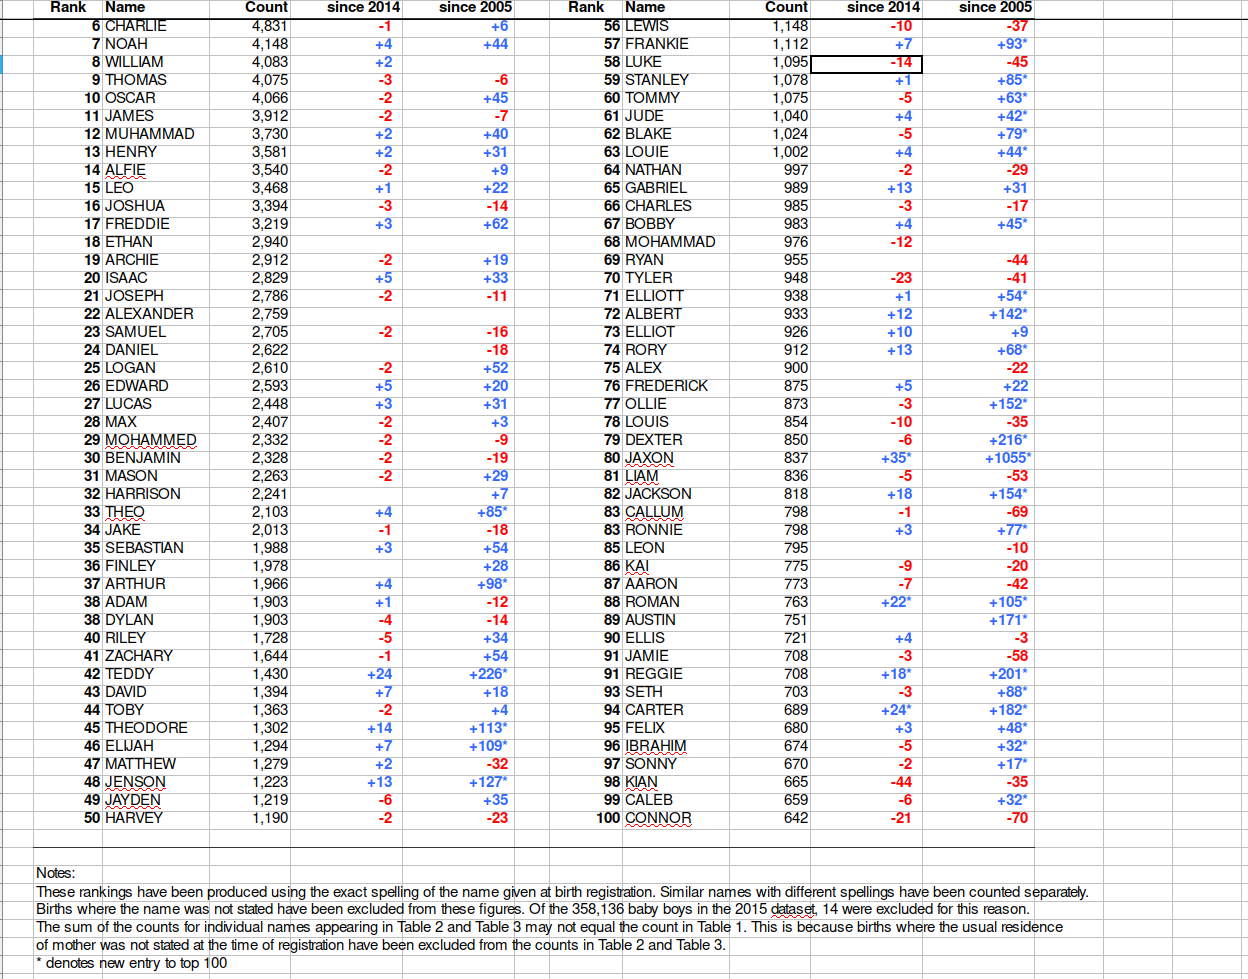
\includegraphics{R/RDataWrangling/images/messy.png}
\caption{messy}
\end{figure}

to this:

\begin{figure}
\centering
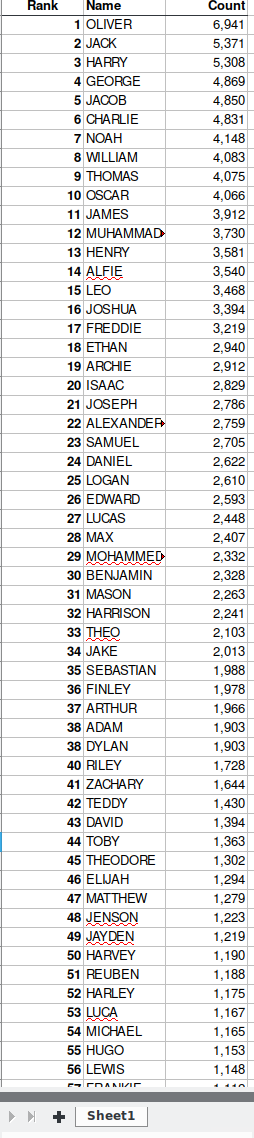
\includegraphics{R/RDataWrangling/images/clean.png}
\caption{tidy}
\end{figure}

There are many ways to do this kind of data manipulation in R. We're
going to use the \emph{dplyr} and \emph{tidyr} packages to make our
lives easier. (Both packages were installed as dependencies of the
\emph{tidyverse} package.)

\subsection{Selecting columns}\label{selecting-columns}

Next we want to retain just the \texttt{Name}, \texttt{Name\_\_1} and
\texttt{Count}, \texttt{Count\_\_1} columns. We can do that using the
\texttt{select} function:

\begin{Shaded}
\begin{Highlighting}[]
\NormalTok{boysNames[[}\DecValTok{1}\NormalTok{]]}

\NormalTok{boysNames[[}\DecValTok{1}\NormalTok{]] <-}\StringTok{ }\KeywordTok{select}\NormalTok{(boysNames[[}\DecValTok{1}\NormalTok{]], Name, Name__}\DecValTok{1}\NormalTok{, Count, Count__}\DecValTok{1}\NormalTok{)}
\NormalTok{boysNames[[}\DecValTok{1}\NormalTok{]]}
\end{Highlighting}
\end{Shaded}

\subsection{Dropping missing values}\label{dropping-missing-values}

Next we want to remove blank rows and rows used for notes. An easy way
to do that is to use \texttt{drop\_na} to remove rows with missing
values.

\begin{Shaded}
\begin{Highlighting}[]
\NormalTok{boysNames[[}\DecValTok{1}\NormalTok{]]}

\NormalTok{boysNames[[}\DecValTok{1}\NormalTok{]] <-}\StringTok{ }\KeywordTok{drop_na}\NormalTok{(boysNames[[}\DecValTok{1}\NormalTok{]])}
\NormalTok{boysNames[[}\DecValTok{1}\NormalTok{]]}
\end{Highlighting}
\end{Shaded}

Finally, we will want to filter out missing do this for all the elements
in \texttt{boysNames}, a task I leave to you.

\section{Exercise 2}\label{exercise-2-3}

\begin{enumerate}
\def\labelenumi{\arabic{enumi}.}
\item
  Write a function that takes a \texttt{data.frame} as an argument and
  returns a modified version including only columns named \texttt{Name},
  \texttt{Name\_\_1}, \texttt{Count}, or \texttt{Count\_\_1}.
\item
  Test your function on the first \texttt{data.frame} in the list of
  baby names data.
\item
  Use the \texttt{map} function to each \texttt{data.frame} in the list
  of baby names data.
\end{enumerate}

\subsection{Re-arranging into a single
table}\label{re-arranging-into-a-single-table}

Our final task is to re-arrange to data so that it is all in a single
table instead of in two side-by-side tables. For many similar tasks the
\texttt{gather} function in the \emph{tidyr} package is useful, but in
this case we will be better off using a combination of \texttt{select}
and \texttt{bind\_rows}.

\begin{Shaded}
\begin{Highlighting}[]
\NormalTok{boysNames[[}\DecValTok{1}\NormalTok{]]}
\KeywordTok{bind_rows}\NormalTok{(}\KeywordTok{select}\NormalTok{(boysNames[[}\DecValTok{1}\NormalTok{]], Name, Count),}
          \KeywordTok{select}\NormalTok{(boysNames[[}\DecValTok{1}\NormalTok{]], }\DataTypeTok{Name =}\NormalTok{ Name__}\DecValTok{1}\NormalTok{, }\DataTypeTok{Count =}\NormalTok{ Count__}\DecValTok{1}\NormalTok{))}
\end{Highlighting}
\end{Shaded}

\section{Exercise 3}\label{exercise-3-2}

\textbf{Cleanup all the data}

In the previous examples we learned how to drop empty rows with
\texttt{filter}, select only relevant columns with \texttt{select}, and
re-arrange our data with \texttt{select} and \texttt{bind\_rows}. In
each case we applied the changes only to the first element of our
\texttt{boysNames} list.

Your task now is to use the \texttt{map} function to apply each of these
transformations to all the elements in \texttt{boysNames}.

\section{Data organization and
storage}\label{data-organization-and-storage}

Now that we have the data cleaned up and augmented, we can turn our
attention to organizing and storing the data.

\subsection{One table for each year}\label{one-table-for-each-year}

Right now we have a list of tables, one for each year. This is not a bad
way to go. It has the advantage of making it easy to work with
individual years; it has the disadvantage of making it more difficult to
examine questions that require data from multiple years. To make the
arrangement of the data clearer it helps to name each element of the
list with the year it corresponds too.

\begin{Shaded}
\begin{Highlighting}[]
\KeywordTok{glimpse}\NormalTok{(}\KeywordTok{head}\NormalTok{(boysNames))}
\end{Highlighting}
\end{Shaded}

\begin{Shaded}
\begin{Highlighting}[]
\NormalTok{years <-}\StringTok{ }\KeywordTok{str_extract}\NormalTok{(boy.file.names, }\StringTok{"[0-9]\{4\}"}\NormalTok{)}
\NormalTok{boysNames <-}\StringTok{ }\KeywordTok{setNames}\NormalTok{(boysNames, years)}
\KeywordTok{glimpse}\NormalTok{(}\KeywordTok{head}\NormalTok{(boysNames))}
\end{Highlighting}
\end{Shaded}

\subsection{One big table}\label{one-big-table}

While storing the data in separate tables by year makes some sense, many
operations will be easier if the data is simply stored in one big table.
We've already seen how to turn a list of data.frames into a single
data.frame using \texttt{bind\_rows}, but there is a problem; The year
information is stored in the names of the list elements, and so
flattening the tables into one will result in losing the year
information! Fortunately it is not too much trouble to add the year
information to each table before flattening.

\begin{Shaded}
\begin{Highlighting}[]
\NormalTok{boysNames <-}\StringTok{ }\KeywordTok{imap}\NormalTok{(boysNames,}
                  \ControlFlowTok{function}\NormalTok{(data, name) \{}
                      \KeywordTok{mutate}\NormalTok{(data, }\DataTypeTok{Year =} \KeywordTok{as.integer}\NormalTok{(name))}
\NormalTok{                      \})}
\NormalTok{boysNames <-}\StringTok{ }\KeywordTok{bind_rows}\NormalTok{(boysNames)}

\KeywordTok{glimpse}\NormalTok{(boysNames)}
\end{Highlighting}
\end{Shaded}

\section{Exercise 4}\label{exercise-4-1}

\textbf{Make one big table}

Turn the list of boys names data.frames into a single table.

Create a directory under \texttt{data/all} and write the data to a
\texttt{.csv} file.

Finally, repeat the previous exercise, this time working with the data
in one big table.

\section{Exercise solutions}\label{exercise-solutions-3}

\subsection{Ex 0: prototype}\label{ex-0-prototype-3}

\begin{quote}
\begin{enumerate}
\def\labelenumi{\arabic{enumi}.}
\tightlist
\item
  Locate the file named \texttt{1996boys\_tcm77-254026.xlsx} and open it
  in a spreadsheet. (If you don't have a spreadsheet program installed
  on your computer you can downloads one from
  \url{https://www.libreoffice.org/download/download/}). What issues can
  you identify that might make working with these data more difficult?
\end{enumerate}
\end{quote}

The data does not start on row one. Headers are on row 7, followed by a
blank line, followed by the actual data.

The data is stored in an inconvenient way, with ranks 1-50 in the first
set of columns and ranks 51-100 in a separate set of columns.

There are notes below the data.

\begin{quote}
\begin{enumerate}
\def\labelenumi{\arabic{enumi}.}
\setcounter{enumi}{2}
\tightlist
\item
  Locate the file named \texttt{2015boysnamesfinal.xlsx} and open it in
  a spreadsheet. In what ways is the format different than the format of
  \texttt{1996boys\_tcm77-254026.xlsx}? How might these differences make
  it more difficult to work with these data?
\end{enumerate}
\end{quote}

The worksheet containing the data of interest is in different positions
and has different names from one year to the next. However, it always
includes ``Table 1'' in the worksheet name.

Some years include columns for ``changes in rank'', others do not.

These differences will make it more difficult to automate re-arranging
the data since we have to write code that can handle different input
formats.

\subsection{Ex 1: prototype}\label{ex-1-prototype-3}

\begin{Shaded}
\begin{Highlighting}[]
\NormalTok{  ## 1. Write a function that takes a file name as an argument and reads}
\NormalTok{  ##    the worksheet containing "Table 1" from that file.}
\NormalTok{  read.baby.names <-}\StringTok{ }\ControlFlowTok{function}\NormalTok{(file) \{}
\NormalTok{      sheet.name <-}\StringTok{ }\KeywordTok{str_subset}\NormalTok{(}\KeywordTok{excel_sheets}\NormalTok{(file), }\StringTok{"Table 1"}\NormalTok{)}
      \KeywordTok{read_excel}\NormalTok{(file, }\DataTypeTok{sheet =}\NormalTok{ sheet.name, }\DataTypeTok{skip =} \DecValTok{6}\NormalTok{)}
\NormalTok{  \}}
  
\NormalTok{  ## 2. Test your function by using it to read *one* of the boys names}
\NormalTok{  ##    Excel files.}
  \KeywordTok{glimpse}\NormalTok{(}\KeywordTok{read.baby.names}\NormalTok{(boy.file.names[}\DecValTok{1}\NormalTok{]))}
     
\NormalTok{  ## 3. Use the `map` function to read data from all the Excel files,}
\NormalTok{  ##    using the function you wrote in step 1.}
\NormalTok{  boysNames <-}\StringTok{ }\KeywordTok{map}\NormalTok{(boy.file.names, read.baby.names)}
\end{Highlighting}
\end{Shaded}

\subsection{Ex 2: prototype}\label{ex-2-prototype-3}

\begin{Shaded}
\begin{Highlighting}[]
\NormalTok{  ## 1. Write a function that takes a `data.frame` as an argument and}
\NormalTok{  ##    returns a modified version including only columns named `Name`,}
\NormalTok{  ##    `Name__1`, `Count`, or `Count__1`.}

\NormalTok{  namecount <-}\StringTok{ }\ControlFlowTok{function}\NormalTok{(data) \{}
      \KeywordTok{select}\NormalTok{(data, Name, Name__}\DecValTok{1}\NormalTok{, Count, Count__}\DecValTok{1}\NormalTok{)}
\NormalTok{  \}}
     
\NormalTok{  ## 2. Test your function on the first `data.frame` in the list of baby}
\NormalTok{  ##    names data.}

  \KeywordTok{namecount}\NormalTok{(boysNames[[}\DecValTok{1}\NormalTok{]])}
  
\NormalTok{  ## 3. Use the `map` function to each `data.frame` in the list of baby}
\NormalTok{  ##    names data.}

\NormalTok{  babyNames <-}\StringTok{ }\KeywordTok{map}\NormalTok{(boysNames, namecount)}
\end{Highlighting}
\end{Shaded}

\subsection{Ex 3: prototype}\label{ex-3-prototype-2}

There are different ways you can go about it. Here is one:

\begin{Shaded}
\begin{Highlighting}[]
\NormalTok{## write a function that does all the cleanup}
\NormalTok{cleanupNamesData <-}\StringTok{ }\ControlFlowTok{function}\NormalTok{(x) \{}
\NormalTok{    filtered <-}\StringTok{ }\KeywordTok{filter}\NormalTok{(x, }\OperatorTok{!}\KeywordTok{is.na}\NormalTok{(Name)) }\CommentTok{# drop rows with no Name value}
\NormalTok{    selected <-}\StringTok{ }\KeywordTok{select}\NormalTok{(filtered, Name, Count, Name__}\DecValTok{1}\NormalTok{, Count__}\DecValTok{1}\NormalTok{) }\CommentTok{# select just Name and Count columns}
    \KeywordTok{bind_rows}\NormalTok{(}\KeywordTok{select}\NormalTok{(selected, Name,  Count), }\CommentTok{# re-arrange into two columns}
              \KeywordTok{select}\NormalTok{(selected, }\DataTypeTok{Name =}\NormalTok{ Name__}\DecValTok{1}\NormalTok{, }\DataTypeTok{Count =}\NormalTok{ Count__}\DecValTok{1}\NormalTok{))}
\NormalTok{\}}

\NormalTok{## test it out on the second data.frame in the list}
\KeywordTok{glimpse}\NormalTok{(boysNames[[}\DecValTok{2}\NormalTok{]]) }\CommentTok{# before cleanup}
\KeywordTok{glimpse}\NormalTok{(}\KeywordTok{cleanupNamesData}\NormalTok{(boysNames[[}\DecValTok{2}\NormalTok{]])) }\CommentTok{# after cleanup}

\NormalTok{## apply the cleanup function to all the data.frames in the list}
\NormalTok{boysNames <-}\StringTok{ }\KeywordTok{map}\NormalTok{(boysNames, cleanupNamesData)}
\end{Highlighting}
\end{Shaded}

\subsection{Ex 4: prototype}\label{ex-4-prototype-1}

Working with the data in one big table is often easier.

\begin{Shaded}
\begin{Highlighting}[]
\NormalTok{boysNames <-}\StringTok{ }\KeywordTok{bind_rows}\NormalTok{(boysNames)}

\KeywordTok{dir.create}\NormalTok{(}\StringTok{"data/all"}\NormalTok{)}

\KeywordTok{write_csv}\NormalTok{(boysNames, }\StringTok{"data/all/boys_names.csv"}\NormalTok{)}

\NormalTok{## What where the five most popular names in 2013?}
\KeywordTok{slice}\NormalTok{(}\KeywordTok{arrange}\NormalTok{(}\KeywordTok{filter}\NormalTok{(boysNames, Year }\OperatorTok{==}\StringTok{ }\DecValTok{2013}\NormalTok{),}
              \KeywordTok{desc}\NormalTok{(Count)),}
      \DecValTok{1}\OperatorTok{:}\DecValTok{5}\NormalTok{)}

\NormalTok{## How has the popularity of the name "ANDREW" changed over time?}
\NormalTok{andrew <-}\StringTok{ }\KeywordTok{filter}\NormalTok{(boysNames, Name }\OperatorTok{==}\StringTok{ "ANDREW"}\NormalTok{)}

\KeywordTok{ggplot}\NormalTok{(andrew, }\KeywordTok{aes}\NormalTok{(}\DataTypeTok{x =}\NormalTok{ Year, }\DataTypeTok{y =}\NormalTok{ Count)) }\OperatorTok{+}
\StringTok{    }\KeywordTok{geom_line}\NormalTok{() }\OperatorTok{+}
\StringTok{    }\KeywordTok{ggtitle}\NormalTok{(}\StringTok{"Popularity of }\CharTok{\textbackslash{}"}\StringTok{Andrew}\CharTok{\textbackslash{}"}\StringTok{, over time"}\NormalTok{)}
\end{Highlighting}
\end{Shaded}

\section{Wrap-up}\label{wrap-up-3}

\subsection{Feedback}\label{feedback-3}

These workshops are a work in progress, please provide any feedback to:
\href{mailto:help@iq.harvard.edu}{\nolinkurl{help@iq.harvard.edu}}

\subsection{Resources}\label{resources-3}

\begin{itemize}
\tightlist
\item
  IQSS

  \begin{itemize}
  \tightlist
  \item
    \href{https://dss.iq.harvard.edu/workshop-materials}{Workshops}
  \item
    \href{https://dss.iq.harvard.edu/}{Data Science Services}
  \item
    \href{https://iqss.github.io/dss-rce/}{Research Computing
    Environment}
  \end{itemize}
\item
  R

  \begin{itemize}
  \tightlist
  \item
    Learn from the best: \url{http://adv-r.had.co.nz/};
    \url{http://r4ds.had.co.nz/}
  \item
    R documentation: \url{http://cran.r-project.org/manuals.html}
  \item
    Collection of R tutorials:
    \url{http://cran.r-project.org/other-docs.html}
  \item
    R for Programmers (by Norman Matloff, UC--Davis)
    \url{http://heather.cs.ucdavis.edu/~matloff/R/RProg.pdf}
  \item
    Calling C and Fortran from R (by Charles Geyer, UMinn)
    \url{http://www.stat.umn.edu/~charlie/rc/}
  \item
    State of the Art in Parallel Computing with R (Schmidberger et al.)
    \url{http://www.jstatso}\textbar{}.org/v31/i01/paper
  \end{itemize}
\end{itemize}

\part{Python}\label{part-python}

\chapter{Python Introduction}\label{python-introduction}

\textbf{Topics}

\begin{itemize}
\tightlist
\item
  Assignment
\item
  Function arguments
\item
  Finding help
\item
  Reading data
\item
  Filtering and arranging data
\item
  Conditional operations
\item
  Saving data
\end{itemize}

\section{Setup}\label{setup-4}

\subsection{Software \& Materials}\label{software-materials-4}

\subsubsection{Install the Anaconda Python
distribution}\label{install-the-anaconda-python-distribution}

If using your own computer please install the Anaconda Python
distribution from \url{https://www.anaconda.com/download/}. (Note that
Python version\(\leq\) 3.0 differs considerably from more recent
releases. For this workshop you will need version\(\geq\) 3.4.)

Accepting the defaults proposed by the Anaconda installer is generally
recommended.

\subsubsection{Download workshop
materials}\label{download-workshop-materials}

Download the materials from
\url{http://tutorials.iq.harvard.edu/Python/PythonIntro.zip} and extract
the zipped directory (Right-click =\textgreater{} Extract All on
Windows, double-click on Mac).

\subsubsection{Launch Jupyter Notebook}\label{launch-jupyter-notebook}

Start the \texttt{Anaconda\ Navigator} program in the usual way. Click
the or \texttt{Launch} button under \texttt{Jupyter\ Notebook}.

\subsection{Goals}\label{goals-4}

In this workshop you will * learn about the python package and
application ecosystem, * learn python language basics and common idioms,
and, * practice reading files and manipulating data in python.

A more general goal is to get you comfortable with Python so that it
seems less scary and mystifying than it perhaps does now. Note that this
is by no means a complete or thorough introduction to Python! It's just
enough to get by.

This workshop is relatively \emph{informal}, \emph{example-oriented},
and \emph{hands-on}. We won't spend much time examining language
features in detail. Instead we will work through an example, and learn
some things about the language along the way.

As an example project we will analyze the text of Lewis Carroll's
\emph{Alice's Adventures in Wonderland}. Among the questions we will use
Python to answer are: * How many total and unique words are there? * How
many chapters and paragraphs? * How many words are in each chapter, and
what is the average words per chapter? * How many times is each main
character mentioned?

\section{What is Python?}\label{what-is-python}

Python is a relatively easy to learn general purpose programming
language. People use Python to manipulate, analyze, and visualize data,
make web sites, write games, and much more. Youtube, DropBox, and
BitTorrent are among the things people used python to make.

Like most popular open source programming languages, Python can be
thought of as a \emph{platform} that runs a huge number and variety of
packages. The language itself is mostly valuable because it makes it
easy to create and use a large number of useful packages.

\section{How can I interact with
Python?}\label{how-can-i-interact-with-python}

A number of interfaces designed to make it easy to interact with Python
are available. The Anaconda distribution that we installed earlier
includes both a web-based \emph{Jupyter Notebook} and a more
conventional Integrated Development Environment called \emph{Spyder}.
For this workshop I encourage you to use \emph{Jupyter Notebook}. In
real life you should experiment and choose the interface that you find
most comfortable.

To get started, start the \emph{Jupyter Notebook} application, and
navigate to the \emph{PythonIntro} directory you downloaded and
extracted earlier. Start a new notebook by clicking
\texttt{New\ =\textgreater{}\ Python\ 3} as shown below.

\begin{figure}
\centering
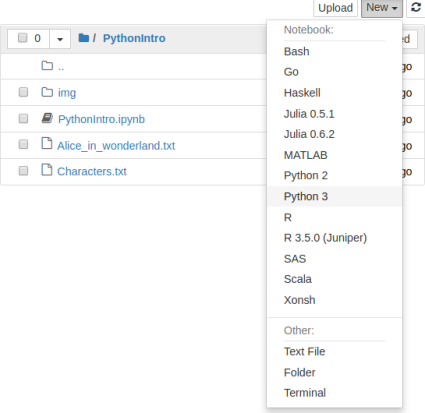
\includegraphics{Python/PythonIntro/images/notebook_new.png}
\caption{notebook\_new.png}
\end{figure}

A Jupyter Notebook contains one or more \emph{cells} containing notes or
code. To insert a new cell click the \texttt{+} button in the upper
left. To execute a cell, select it and press \texttt{Control+Enter} or
click the \texttt{Run} button at the top.

\section{Reading the text of Alice in Wonderland from a
file}\label{reading-the-text-of-alice-in-wonderland-from-a-file}

Reading information from a file is the first step in many projects, so
we'll start there. The workshop materials you downloaded earlier include
a file named \texttt{Alice\_in\_wonderland.txt} which contains the text
of Lewis Carroll's \emph{Alice's Adventures in Wonderland}.

We can open a connection to a file using the \emph{open} function, and
store the result using the \texttt{=} operator.

\begin{Shaded}
\begin{Highlighting}[]
\NormalTok{alice_file }\OperatorTok{=} \BuiltInTok{open}\NormalTok{(}\StringTok{"Alice_in_wonderland.txt"}\NormalTok{)}
\end{Highlighting}
\end{Shaded}

The name on the left of the equals sign (\texttt{alice\_file}) is one
that we chose. When choosing names, \emph{start with a letter}, and use
only \emph{letters}, \emph{numbers} and \emph{underscores}.

The \texttt{alice\_file} object we just created does \emph{not} contain
the contents of \texttt{Alice\_in\_wonderland.txt}. It a representation
in Python of the \emph{file itself} rather than the \emph{contents} of
the file.

The \texttt{alice\_file} object provides \emph{methods} that we can use
to do things with it. Methods are invoked using syntax that looks like
\texttt{ObjectName.method()}. You can see the methods available for
acting on an object by typing the object's name followed by a \texttt{.}
and pressing the \texttt{tab} key. For example, typing
\texttt{alice\_file.} and pressing \texttt{tab} will display a list of
methods as shown below.
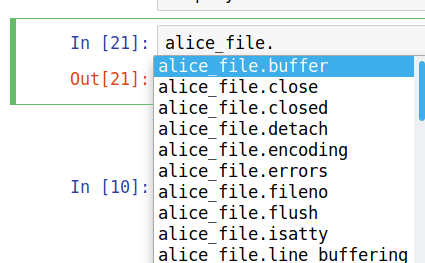
\includegraphics{Python/PythonIntro/images/notebook_file_completion.png}.

Among the methods we have for doing things with our \texttt{alice\_file}
object is one named \texttt{read}. We can use the \texttt{help} function
to learn more about it.

\begin{Shaded}
\begin{Highlighting}[]
\BuiltInTok{help}\NormalTok{(alice_file.read)}
\end{Highlighting}
\end{Shaded}

Since \texttt{alice\_file.read} looks promising, we will invoke this
method and see what it does.

\begin{Shaded}
\begin{Highlighting}[]
\NormalTok{alice_txt }\OperatorTok{=}\NormalTok{ alice_file.read()}
\BuiltInTok{print}\NormalTok{(alice_txt[:}\DecValTok{500}\NormalTok{]) }\CommentTok{# the [:500] gets the first 500 character -- more on this later.}
\end{Highlighting}
\end{Shaded}

That's all there is to it! We've read the contents of
\texttt{Alice\_in\_wonderland.txt} and stored this text in a Python
object we named \texttt{alice\_txt}. Now let's start to explore this
object, and learn some more things about Python along the way.

\section{Counting chapters, lines, and
words}\label{counting-chapters-lines-and-words}

Now that we have the text we can start answering some questions about
it. To begin with, how many words does it contain? To answer this
question we can split the text up so there is one element per word, and
then count the number of words.

\subsection{Splitting a string into a list of
words}\label{splitting-a-string-into-a-list-of-words}

How do we figure out how to split strings in Python? By asking Python
what our \texttt{alice\_txt} object is and what methods it provides. We
can ask Python what things are using the \texttt{type} function, like
this:

\begin{Shaded}
\begin{Highlighting}[]
\BuiltInTok{type}\NormalTok{(alice_txt)}
\end{Highlighting}
\end{Shaded}

Python tells us that \texttt{alice\_txt} is of type \texttt{str} (i.e.,
it is a string). We can find out what methods are available for working
strings by typing \texttt{alice\_txt.} and pressing \texttt{tab}. We'll
see that among the methods is one named \texttt{split}, as shown below.
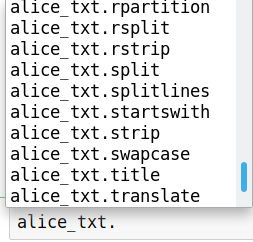
\includegraphics{Python/PythonIntro/images/notebook_string_completion.png}
To learn how to use this method we can check the documentation.

\begin{Shaded}
\begin{Highlighting}[]
\BuiltInTok{help}\NormalTok{(alice_txt.split)}
\end{Highlighting}
\end{Shaded}

Since the default is to split on whitespace (spaces, newlines, tabs) we
can get a reasonable word count simply by calling the split method and
counting the number of elements in the result.

\begin{Shaded}
\begin{Highlighting}[]
\NormalTok{alice_words }\OperatorTok{=}\NormalTok{ alice_txt.split()}
\BuiltInTok{len}\NormalTok{(alice_words)}
\end{Highlighting}
\end{Shaded}

\subsection{Using sets to calculate the number of unique
words}\label{using-sets-to-calculate-the-number-of-unique-words}

According to our computation above, there are about 26 thousand total
words in \emph{Alice's Adventures in Wonderland}. But how many
\emph{unique} words are there? Python has a special data structure
called a \emph{set} that makes it easy to find out. A \emph{set} drops
all duplicates, giving a collection of the unique elements.

\begin{Shaded}
\begin{Highlighting}[]
\BuiltInTok{len}\NormalTok{(}\BuiltInTok{set}\NormalTok{(alice_words))}
\end{Highlighting}
\end{Shaded}

There are 5295 unique words in the text.

\section{Exercise: Reading text from a file and
splitting}\label{exercise-reading-text-from-a-file-and-splitting}

\emph{Alice's Adventures in Wonderland} is full of memorable characters.
The main characters from the story are listed, one-per-line, in the file
named \texttt{Characters.txt}.

NOTE: we will not always explicitly demonstrate everything you need to
know in order to complete an exercise. Instead we focus on teaching you
how to discover available methods and how use the help function to learn
how to use them. It is expected that you will spend some time during the
exercises looking for appropriate methods and perhaps reading
documentation.

\begin{enumerate}
\def\labelenumi{\arabic{enumi}.}
\item
  Open the \texttt{Characters.txt} file and read its contents.
\item
  Split text on newlines to produce a list with one element per line.
  Store the result as ``alice\_characters''.
\end{enumerate}

```

\subsection{Working with lists}\label{working-with-lists}

The \texttt{split} methods we used to break up the text of \emph{Alice
in Wonderland} into words produced a \emph{list}. A lot of the
techniques we'll use later to analyze this text also produce lists, so
its worth taking a minute to learn more about them.

It is always a good idea to know what type of things you're working with
in Python. As you gain experience, you won't have to look this things up
as often, but even experienced Python programmers use the \texttt{type}
function to learn about the objects they are working with.

\begin{Shaded}
\begin{Highlighting}[]
\BuiltInTok{type}\NormalTok{(alice_words)}
\end{Highlighting}
\end{Shaded}

A \emph{list} in Python is used to store a collection of items. As with
other types in Python, you can get a list of methods by typing the name
of the object followed by a \texttt{.} and pressing \texttt{tab}.

\subsubsection{Extracting subsets from
lists}\label{extracting-subsets-from-lists}

Among the things you can do with a list is extract subsets using bracket
indexing notation. This is useful in many situations, including the
current one where we want to inspect a long list without printing out
the whole thing.

The examples below show how indexing works in Python.

\begin{Shaded}
\begin{Highlighting}[]
\NormalTok{alice_words[}\DecValTok{0}\NormalTok{] }\CommentTok{# first word (yes, we count from zero!)}
\end{Highlighting}
\end{Shaded}

\begin{Shaded}
\begin{Highlighting}[]
\NormalTok{alice_words[}\DecValTok{1}\NormalTok{] }\CommentTok{# second word}
\end{Highlighting}
\end{Shaded}

\begin{Shaded}
\begin{Highlighting}[]
\NormalTok{alice_words[:}\DecValTok{10}\NormalTok{] }\CommentTok{# first 10 words}
\end{Highlighting}
\end{Shaded}

\begin{Shaded}
\begin{Highlighting}[]
\NormalTok{alice_words[}\DecValTok{10}\NormalTok{:}\DecValTok{20}\NormalTok{] }\CommentTok{# words 11 through 20}
\end{Highlighting}
\end{Shaded}

\begin{Shaded}
\begin{Highlighting}[]
\NormalTok{alice_words[}\OperatorTok{-}\DecValTok{1}\NormalTok{] }\CommentTok{# the last word}
\end{Highlighting}
\end{Shaded}

\begin{Shaded}
\begin{Highlighting}[]
\NormalTok{alice_words[}\OperatorTok{-}\DecValTok{10}\NormalTok{:] }\CommentTok{# the last 10 words}
\end{Highlighting}
\end{Shaded}

Note that the displayed representation of lists and other data
structures in python often closely matches the syntax used to create
them. For example, we can create a list using square brackets, just as
we see when we print a list:

\begin{Shaded}
\begin{Highlighting}[]
\NormalTok{[}\StringTok{'her'}\NormalTok{,}
 \StringTok{'own'}\NormalTok{,}
 \StringTok{'child-life,'}\NormalTok{,}
 \StringTok{'and'}\NormalTok{,}
 \StringTok{'the'}\NormalTok{,}
 \StringTok{'happy'}\NormalTok{,}
 \StringTok{'summer'}\NormalTok{,}
 \StringTok{'days.'}\NormalTok{,}
 \StringTok{'THE'}\NormalTok{,}
 \StringTok{'END'}\NormalTok{]}
\end{Highlighting}
\end{Shaded}

\subsubsection{Sorting and other in-place
methods}\label{sorting-and-other-in-place-methods}

There are many other things we can do with lists besides extracting
subsets using bracket indexing. For example, there are methods to append
and remove elements from a list. When using a list method that you are
unfamiliar with, it is always a good idea to read the documentation.

Note that many methods modify the object \emph{in place}. For example,
if we wanted to sort the last 10 words in \texttt{alice\_words} we would
do it like this:

\begin{Shaded}
\begin{Highlighting}[]
\NormalTok{last_10 }\OperatorTok{=}\NormalTok{ alice_words[}\OperatorTok{-}\DecValTok{10}\NormalTok{:]}
\BuiltInTok{print}\NormalTok{(last_10)}
\NormalTok{last_10.sort()}
\BuiltInTok{print}\NormalTok{(last_10)}
\end{Highlighting}
\end{Shaded}

\subsection{Counting chapters and
paragraphs}\label{counting-chapters-and-paragraphs}

Now that we know how to split a string and how to work with the
resulting list, we can split on chapter markers to count the number of
chapters. All we need to do is specify the string to split on. Since
each chapter is marked with the string
\texttt{\textquotesingle{}CHAPTER\ \textquotesingle{}} followed by the
chapter number, we can split the text up into chapters using this as the
separator.

\begin{Shaded}
\begin{Highlighting}[]
\NormalTok{alice_chapters }\OperatorTok{=}\NormalTok{ alice_txt.split(}\StringTok{"CHAPTER "}\NormalTok{)}
\BuiltInTok{len}\NormalTok{(alice_chapters)}
\end{Highlighting}
\end{Shaded}

Since the first element contains the material \emph{before} the first
chapter, this tells us there are twelve chapters in the book.

We can count paragraphs in a similar way. Paragraphs are indicated by a
blank line, i.e., two newlines in a row. When working with strings we
can represent newlines with \texttt{\textbackslash{}n}, so our basic
paragraph separator is \texttt{\textbackslash{}n\textbackslash{}n}.

\begin{Shaded}
\begin{Highlighting}[]
\NormalTok{alice_paragraphs }\OperatorTok{=}\NormalTok{ alice_txt.split(}\StringTok{"}\CharTok{\textbackslash{}n\textbackslash{}n}\StringTok{"}\NormalTok{)}
\end{Highlighting}
\end{Shaded}

Before counting the number of paragraphs, I want to inspect the result
to see if it looks correct:

\begin{Shaded}
\begin{Highlighting}[]
\BuiltInTok{print}\NormalTok{(alice_paragraphs[}\DecValTok{0}\NormalTok{], }\StringTok{"}\CharTok{\textbackslash{}n}\StringTok{=========="}\NormalTok{)}
\BuiltInTok{print}\NormalTok{(alice_paragraphs[}\DecValTok{1}\NormalTok{], }\StringTok{"}\CharTok{\textbackslash{}n}\StringTok{=========="}\NormalTok{)}
\BuiltInTok{print}\NormalTok{(alice_paragraphs[}\DecValTok{2}\NormalTok{], }\StringTok{"}\CharTok{\textbackslash{}n}\StringTok{=========="}\NormalTok{)}
\BuiltInTok{print}\NormalTok{(alice_paragraphs[}\DecValTok{3}\NormalTok{], }\StringTok{"}\CharTok{\textbackslash{}n}\StringTok{=========="}\NormalTok{)}
\BuiltInTok{print}\NormalTok{(alice_paragraphs[}\DecValTok{4}\NormalTok{], }\StringTok{"}\CharTok{\textbackslash{}n}\StringTok{=========="}\NormalTok{)}
\BuiltInTok{print}\NormalTok{(alice_paragraphs[}\DecValTok{5}\NormalTok{], }\StringTok{"}\CharTok{\textbackslash{}n}\StringTok{=========="}\NormalTok{)}
\end{Highlighting}
\end{Shaded}

We're counting the title, author, and chapter lines as paragraphs, but
this will do for a rough count.

\begin{Shaded}
\begin{Highlighting}[]
\BuiltInTok{len}\NormalTok{(alice_paragraphs)}
\end{Highlighting}
\end{Shaded}

\section{Exercise: count the number of main
characters}\label{exercise-count-the-number-of-main-characters}

So far we've learned that there are 12 chapters, around 830 paragraphs,
and about 26 thousand words in \emph{Alice's Adventures in Wonderland}.
Along the way we've also learned how to open a file and read its
contents, split strings, calculate the length of objects, discover
methods for string and list objects, and index/subset lists in Python.
Now it is time for you to put these skills to use to learn something
about the main characters in the story.

\begin{enumerate}
\def\labelenumi{\arabic{enumi}.}
\item
  Count the number of main characters in the story (i.e., get the length
  of the list you created in previous exercise).
\item
  Extract and print just the first character from the list you created
  in the previous exercise.
\item
  (BONUS, optional): Sort the list you created in step 2 alphabetically,
  and then extract the last element.
\end{enumerate}

\section{Working with nested structures: words within paragraphs within
chapters}\label{working-with-nested-structures-words-within-paragraphs-within-chapters}

This far our analysis as treated the text as a ``flat'' data structure.
For example, when we counted words we just counted words in the whole
document, rather than counting the number of words in each chapter. If
we want to treat our document as a nested structure, with words forming
sentences, sentences forming paragraphs, paragraphs forming chapters,
and chapters forming the book, we need to learn some additional tools.
Specifically, we need to learn how to iterate over lists (or other
collections) and do things with each element in a collection.

There are several ways to iterate in Python, of which we will focus on
\emph{for loops} and \emph{list comprehensions}.

\subsection{Iterating over paragraphs using
for-loops}\label{iterating-over-paragraphs-using-for-loops}

A \emph{for loop} is a way of cycling through the elements of a
collection and doing something with each one. As a simple example, we
can cycle through the first 6 paragraphs and print each one. Cycling
through with a loop makes it easy to insert a separator between the
paragraphs, making it much easier to read the output.

\begin{Shaded}
\begin{Highlighting}[]
\ControlFlowTok{for}\NormalTok{ paragraph }\KeywordTok{in}\NormalTok{ alice_paragraphs[:}\DecValTok{6}\NormalTok{]:}
    \BuiltInTok{print}\NormalTok{(paragraph)}
    \BuiltInTok{print}\NormalTok{(}\StringTok{'=================================='}\NormalTok{)}
\BuiltInTok{print}\NormalTok{(}\StringTok{'DONE.'}\NormalTok{)}
\end{Highlighting}
\end{Shaded}

Notice that the syntax of a for-loop is

\begin{verbatim}
for <thing> in <collection>:
    do stuff with <thing>
\end{verbatim}

Notice also that the body of the for-loop is indented. This is
important, because it is this indentation that defines the body of the
loop. Notice that ``DONE.'' is only printed once, since
\texttt{print(\textquotesingle{}DONE.\textquotesingle{})} is not
indented and is therefore outside of the body of the loop.

Loops in Python are great because the syntax is relatively simple, and
because they are very powerful. Inside of the body of a loop you can use
all the tools you use elsewhere in python.

Here is one more example of a loop, this time iterating over all the
chapters and calculating the number of paragraphs in each chapter.

\begin{Shaded}
\begin{Highlighting}[]
\ControlFlowTok{for}\NormalTok{ chapter }\KeywordTok{in}\NormalTok{ alice_chapters[}\DecValTok{1}\NormalTok{:]:}
\NormalTok{    paragraphs }\OperatorTok{=}\NormalTok{ chapter.split(}\StringTok{"}\CharTok{\textbackslash{}n\textbackslash{}n}\StringTok{"}\NormalTok{)}
    \BuiltInTok{print}\NormalTok{(}\BuiltInTok{len}\NormalTok{(paragraphs))}
\end{Highlighting}
\end{Shaded}

\subsection{Iterating and collecting paragraphs per chapter using list
comprehension}\label{iterating-and-collecting-paragraphs-per-chapter-using-list-comprehension}

We could use for-loops to fill in lists of values, but there is a
special syntax in Python that is often better for this use case. This
special syntax is called a \emph{list comprehension} and it looks like
this:

\begin{Shaded}
\begin{Highlighting}[]
\NormalTok{paragraphs_per_chapter }\OperatorTok{=}\NormalTok{ [}\BuiltInTok{len}\NormalTok{(chapter.split(}\StringTok{"}\CharTok{\textbackslash{}n\textbackslash{}n}\StringTok{"}\NormalTok{)) }
                          \ControlFlowTok{for}\NormalTok{ chapter }\KeywordTok{in}\NormalTok{ alice_chapters[}\DecValTok{1}\NormalTok{:]]}
\BuiltInTok{print}\NormalTok{(paragraphs_per_chapter)}
\end{Highlighting}
\end{Shaded}

Notice that \emph{list comprehension} is very similar to a \emph{for
loop}, though the order is different. In a \emph{for-loop} the
\texttt{for} part comes first and the expressions that make up the body
come second and are indented. In a \emph{list comprehension} the
expression comes first and the \texttt{for} part comes afterward. Notice
also the square brackets surrounding the whole thing -- these brackets
are what tells Python that you want a list.

Here is another list comprehension that counts the number of times the
name ``Alice'' appears in each chapter.

\begin{Shaded}
\begin{Highlighting}[]
\NormalTok{alices_per_chapter }\OperatorTok{=}\NormalTok{ [chapter.count(}\StringTok{"Alice"}\NormalTok{) }\ControlFlowTok{for}\NormalTok{ chapter }\KeywordTok{in}\NormalTok{ alice_chapters]}
\BuiltInTok{print}\NormalTok{(alices_per_chapter)}
\end{Highlighting}
\end{Shaded}

\subsection{Organizing results in
dictionaries}\label{organizing-results-in-dictionaries}

Our code for calculating the number of of times ``Alice'' was mentioned
per chapter worked, but with a little effort we can make it much easier
to interpret by associating each count with the chapter it corresponds
to. In Python we can use a \texttt{dict} (i.e., ``dictionary'') to store
key-value pairs.

First, we can iterate over each chapter and grab just the first line
(that is, the chapter titles). These will become our keys.

\begin{Shaded}
\begin{Highlighting}[]
\NormalTok{chapter_names }\OperatorTok{=}\NormalTok{ [chapter.splitlines()[}\DecValTok{0}\NormalTok{] }\ControlFlowTok{for}\NormalTok{ chapter }\KeywordTok{in}\NormalTok{ alice_chapters[}\DecValTok{1}\NormalTok{:]]}
\BuiltInTok{print}\NormalTok{(chapter_names)}
\end{Highlighting}
\end{Shaded}

Finally we can combine the chapter titles and counts and convert them to
a dictionary.

\begin{Shaded}
\begin{Highlighting}[]
\BuiltInTok{dict}\NormalTok{(}\BuiltInTok{zip}\NormalTok{(chapter_names, }
\NormalTok{         [chapter.count(}\StringTok{"Alice"}\NormalTok{) }
          \ControlFlowTok{for}\NormalTok{ chapter }\KeywordTok{in}\NormalTok{ alice_chapters]))}
\end{Highlighting}
\end{Shaded}

\section{Exercise: Iterating and counting
things}\label{exercise-iterating-and-counting-things}

Now that we know how to iterate using for-loops and list comprehensions
the possibilities really start to open up. For example, we can use these
techniques to count the number of times each character appears in the
story.

\begin{enumerate}
\def\labelenumi{\arabic{enumi}.}
\tightlist
\item
  Make sure you have both the text and the list of characters.
\end{enumerate}

Open and read both ``Alice\_in\_wonderland.txt'' and ``Characters.txt''
if you have not already done so.

\begin{enumerate}
\def\labelenumi{\arabic{enumi}.}
\setcounter{enumi}{1}
\tightlist
\item
  Which chapter has the most words?
\end{enumerate}

Split the text into chaptes (i.e., split on ``CHAPTER'') and use a
for-loop or list comprehension to iterate over the chapters. For each
chapter, split it into words and calculate the length.

\begin{enumerate}
\def\labelenumi{\arabic{enumi}.}
\setcounter{enumi}{2}
\tightlist
\item
  How many times is each character mentioned in the text?
\end{enumerate}

Iterate over the list of characters using a for-loop or list
comprehension. For each character, call the count method with that
character as the argument.

\begin{enumerate}
\def\labelenumi{\arabic{enumi}.}
\setcounter{enumi}{3}
\tightlist
\item
  (BONUS, optional): Put the character counts computed above in a
  dictionary with character names as the keys and counts as the values.
\item
  (BONUS, optional): Use a nested list comprehension to calculate the
  number of times each character is mentioned in each chapter.
\end{enumerate}

\section{Importing numpy and calculating simple
statistics}\label{importing-numpy-and-calculating-simple-statistics}

Now that we know how to iterate over lists and calculate numbers for
each element, we may wish to do some simple math using these numbers.
For example, we may want to calculate the mean and standard deviation of
the distribution of the number of paragraphs in each chapter. Python has
a handful of math functions built-in (e.g., \texttt{min} and
\texttt{max}) but built-in math support is pretty limited.

When you find that something isn't available in Python itself, its time
to look for a package that does it. Although it is somewhat overkill for
simply calculating a mean we're going to use a popular package called
\emph{numpy} for this. The \emph{numpy} package is included in the
Anaconda Python distribution we are using, so we don't need to install
it separately.

In order to use \emph{numpy} or other packages, you must first import
them. We can import numpy as follows:

\begin{Shaded}
\begin{Highlighting}[]
\ImportTok{import}\NormalTok{ numpy}
\end{Highlighting}
\end{Shaded}

The \emph{numpy} package is very popular and includes a lot of useful
functions. For example, we can use it to calculate means and standard
deviations:

\begin{Shaded}
\begin{Highlighting}[]
\BuiltInTok{print}\NormalTok{(numpy.mean(paragraphs_per_chapter))}
\BuiltInTok{print}\NormalTok{(numpy.std(paragraphs_per_chapter))}
\end{Highlighting}
\end{Shaded}

and compute correlations:

\begin{Shaded}
\begin{Highlighting}[]
\NormalTok{words_per_chapter }\OperatorTok{=}\NormalTok{ [}\BuiltInTok{len}\NormalTok{(chapter.split()) }\ControlFlowTok{for}\NormalTok{ chapter }\KeywordTok{in}\NormalTok{ alice_chapters]}
\NormalTok{alices_per_chapter }\OperatorTok{=}\NormalTok{ [chapter.count(}\StringTok{"Alice"}\NormalTok{) }\ControlFlowTok{for}\NormalTok{ chapter }\KeywordTok{in}\NormalTok{ alice_chapters]}

\BuiltInTok{print}\NormalTok{(numpy.corrcoef(words_per_chapter, alices_per_chapter))}
\end{Highlighting}
\end{Shaded}

\section{Wrap-up}\label{wrap-up-4}

\subsection{Feedback}\label{feedback-4}

Please take 60 seconds to fill out a very short feedback
\href{http://bit.ly/training_class_eval}{form}

\subsection{Resources}\label{resources-4}

\begin{itemize}
\tightlist
\item
  IQSS

  \begin{itemize}
  \tightlist
  \item
    \href{https://dss.iq.harvard.edu/workshop-materials}{Workshops}
  \item
    \href{https://dss.iq.harvard.edu/}{Data Science Services}
  \item
    \href{https://iqss.github.io/dss-rce/}{Research Computing
    Environment}
  \end{itemize}
\item
  Graphics

  \begin{itemize}
  \tightlist
  \item
    \href{https://matplotlib.org/}{matplotlib}
  \item
    \href{https://seaborn.pydata.org/}{seaborn}
  \item
    \href{https://plot.ly/python/}{plotly}
  \end{itemize}
\item
  Quantitative Data Analysis

  \begin{itemize}
  \tightlist
  \item
    \href{http://www.numpy.org/}{numpy}
  \item
    \href{https://www.scipy.org/}{scipy}
  \item
    \href{https://pandas.pydata.org/}{pandas}
  \item
    \href{http://scikit-learn.org/stable/}{scikit-learn}
  \item
    \href{http://www.statsmodels.org/stable/}{statsmodels}
  \end{itemize}
\item
  Text analysis

  \begin{itemize}
  \tightlist
  \item
    \href{https://textblob.readthedocs.io/en/dev/}{textblob}
  \item
    \href{http://www.nltk.org/}{nltk}
  \item
    \href{https://radimrehurek.com/gensim/}{Gensim}
  \end{itemize}
\item
  Webscraping

  \begin{itemize}
  \tightlist
  \item
    \href{https://scrapy.org/}{scrapy}
  \item
    \href{http://docs.python-requests.org/en/master/}{requests}
  \item
    \href{https://lxml.de/}{lxml}
  \item
    \href{https://www.crummy.com/software/BeautifulSoup/}{BeautifulSoup}
  \end{itemize}
\item
  Social Network Analysis

  \begin{itemize}
  \tightlist
  \item
    \href{https://networkx.github.io/}{networkx}
  \item
    \href{https://graph-tool.skewed.de/}{graph-tool}
  \end{itemize}
\end{itemize}

\chapter{Python Web-Scraping}\label{python-web-scraping}

\textbf{Topics}

\begin{itemize}
\tightlist
\item
  Assignment
\item
  Function arguments
\item
  Finding help
\item
  Reading data
\item
  Filtering and arranging data
\item
  Conditional operations
\item
  Saving data
\end{itemize}

\section{Setup}\label{setup-5}

\subsection{Software \& Materials}\label{software-materials-5}

\subsubsection{Install the Anaconda Python
distribution}\label{install-the-anaconda-python-distribution-1}

If using your own computer please install the Anaconda Python
distribution from \url{https://www.anaconda.com/download/}. (Note that
Python version \(\leq\) 3.0 differs considerably from more recent
releases. For this workshop you will need version \(\geq\) 3.4.)

Accepting the defaults proposed by the Anaconda installer is generally
recommended.

\subsubsection{Workshop notes}\label{workshop-notes}

The class notes for this workshop are available on our website at
\href{https://dss.iq.harvard.edu}{dss.iq.harvard.edu} under
\texttt{Workshop\ Materials\ ==\textgreater{}\ Python\ Workshop\ Materials\ =\textgreater{}\ Python\ Web\ Scraping}.
Click the \texttt{All\ workshop\ materials} link to download the
workshop materials.

Extract the \texttt{PythonWebScraping.zip} directory
(\texttt{Right-click\ =\textgreater{}\ Extract\ All} on Windows,
\texttt{double-click} on Mac).

Start the \texttt{Jupyter\ Notebook} application and open the
\texttt{Exercises.ipynb} file in the \texttt{PythonWebScraping} folder
you downloaded previously. You may also wish to start a new notebook for
your own notes.

\subsection{Goals}\label{goals-5}

In this workshop you will

\begin{itemize}
\tightlist
\item
  learn basic web scraping principles and techniques,
\item
  learn how to use the \texttt{requests} package in Python,
\item
  practice making requests and manipulating responses from the server.
\end{itemize}

This workshop is relatively \emph{informal}, \emph{example-oriented},
and \emph{hands-on}. We will learn by working through an example web
scraping project.

Note that this is \textbf{not} an introductory workshop. Familiarity
with Python, including but not limited to knowledge of lists and
dictionaries, indexing, and loops and / or comprehensions is assumed. If
you need an introduction to Python or a refresher, we recommend the
\href{https://dss.iq.harvard.edu/workshop-materials\#widget-0}{IQSS
Introduction to Python}.

Note also that this workshop will not teach you everything you need to
know in order to retrieve data from any web service you might wish to
scrape. You can expect to learn just enough to be dangerous.

\section{Preliminary questions}\label{preliminary-questions}

\subsection{What is web scraping?}\label{what-is-web-scraping}

Web scraping is the activity of automating retrieval of information from
a web service designed for human interaction.

\subsection{Is web scraping legal? Is it
ethical?}\label{is-web-scraping-legal-is-it-ethical}

It depends. If you have legal questions seek legal counsel. You can
mitigate some ethical issues by building delays and restrictions into
your web scraping program so as to avoid impacting the availability of
the web service for other users or the cost of hosting the service for
the service provider.

\section{Example project}\label{example-project-1}

In this workshop I will demonstrate web scraping techniques using the
Collections page at \url{https://www.harvardartmuseums.org/collections}
and let you use the skills you'll learn to retrieve information from
other parts of the Harvard Art Museums website.

The basic strategy is pretty much the same for most scraping projects.
We will use our web browser (Chrome or Firefox recommended) to examine
the page you wish to retrieve data from, and copy/paste information from
your web browser into your scraping program.

\section{Take shortcuts if you can}\label{take-shortcuts-if-you-can}

We wish to extract information from
\url{https://www.harvardartmuseums.org/collections}. Like most modern
web pages, a lot goes on behind the scenes to produce the page we see in
our browser. Our goal is to pull back the curtain to see what the
website does when we interact with it. Once we see how the website works
we can start retrieving data from it. If we are lucky we'll find a
resource that returns the data we're looking for in a structured format
like \href{https://json.org/}{JSON} or
\href{https://en.wikipedia.org/wiki/XML}{XML}.

\subsection{Examining the structure of our target web
service}\label{examining-the-structure-of-our-target-web-service}

We start by opening the collections web page in a web browser and
inspecting it.

\begin{figure}
\centering
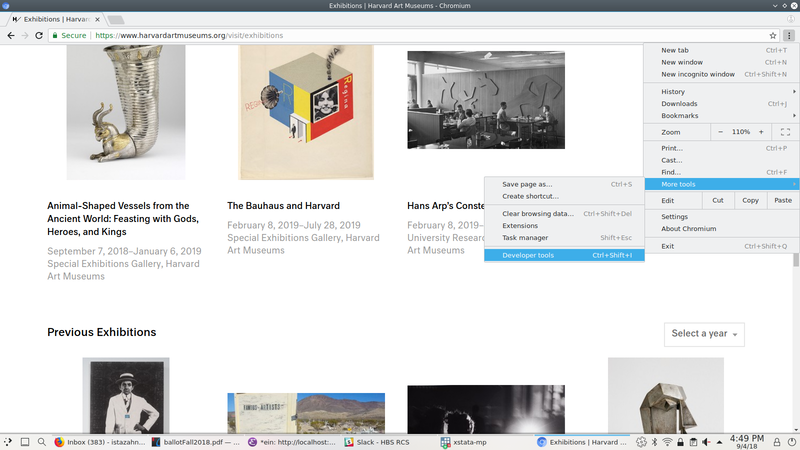
\includegraphics{Python/PythonWebScrape/images/dev_tools.png}
\caption{}
\end{figure}

\begin{figure}
\centering
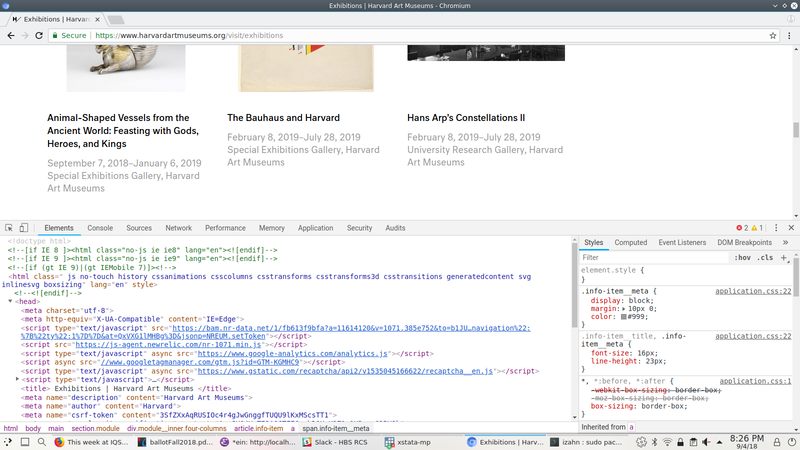
\includegraphics{Python/PythonWebScrape/images/dev_tools_pane.png}
\caption{}
\end{figure}

If we scroll down to the bottom of the Collections page, we'll see a
button that says ``Load More''. Let's see what happens when we click on
that button. To do so, click on ``Network'' in the developer tools
window, then click the ``Load More Collections'' button. You should see
a list of requests that were made as a result of clicking that button,
as shown below.

\begin{figure}
\centering
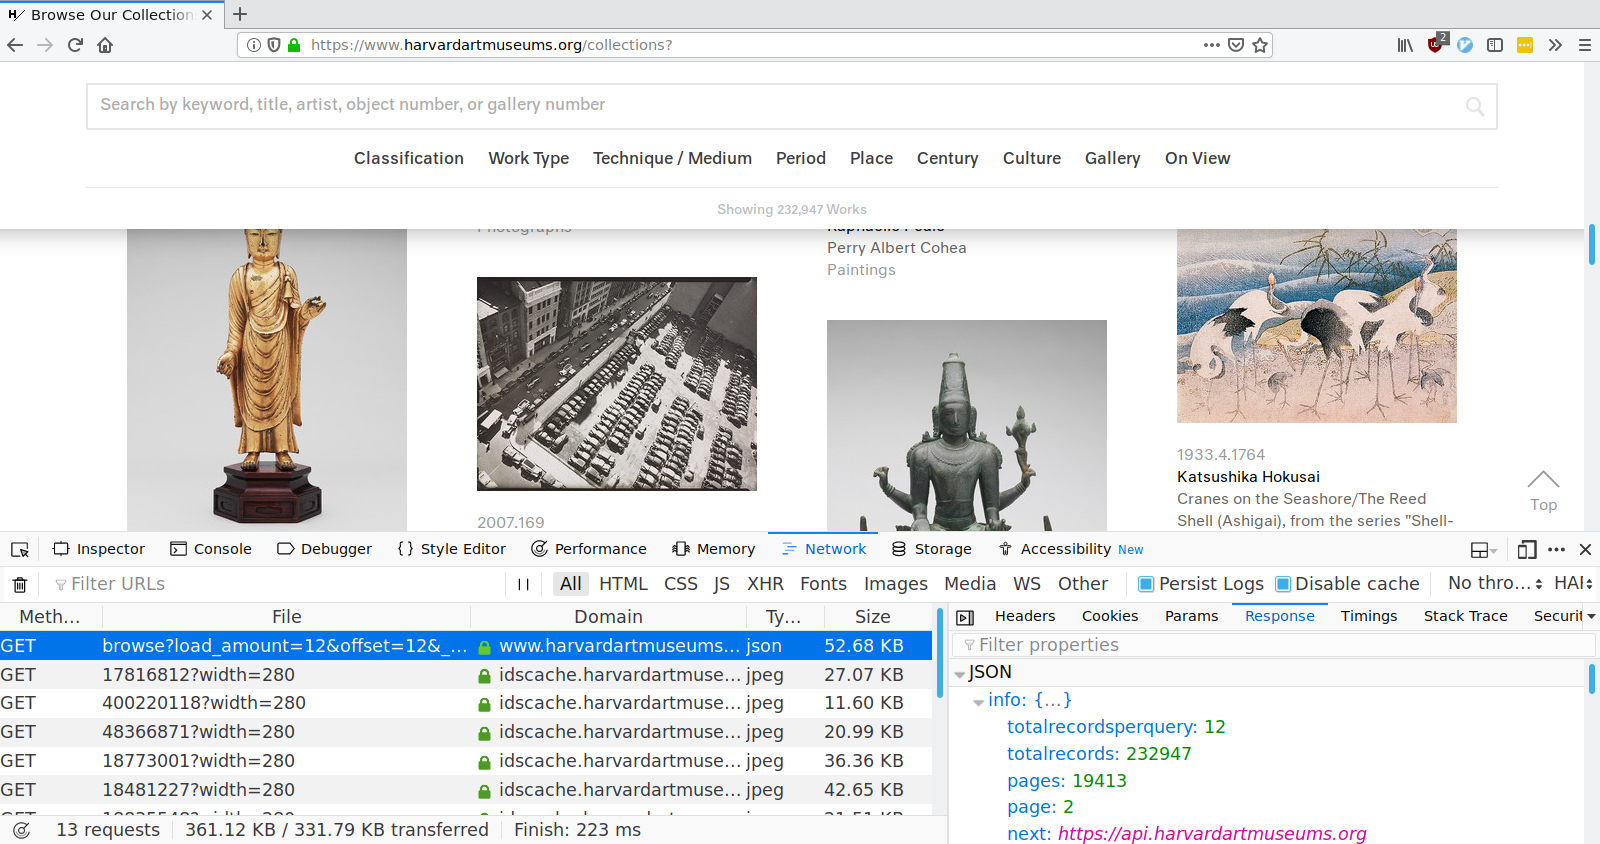
\includegraphics{Python/PythonWebScrape/images/dev_tools_network.png}
\caption{}
\end{figure}

If we look at that second request, the one to a script named
\texttt{browse}, we'll see that it returns all the information we need,
in a convenient format called \texttt{JSON}. All we need to retrieve
collection data is call make \texttt{GET} requests to
\url{https://www.harvardartmuseums.org/browse} with the correct
parameters.

\subsection{Making requests using
python}\label{making-requests-using-python}

The URL we want to retrieve data from has the following structure

\begin{verbatim}
scheme                    domain    path  parameters
 https www.harvardartmuseums.org  browse  load_amount=10&offset=0
\end{verbatim}

It is often convenient to create variables containing the domain(s) and
path(s) you'll be working with, as this allows you to swap out paths and
parameters as needed. Note that the path is separated from the domain
with \texttt{/} and the parameters are separated from the path with
\texttt{?}. If there are multiple parameters they are separated from
each other with a \texttt{\&}.

For example, we can define the domain and path of the collections URL as
follows:

\begin{Shaded}
\begin{Highlighting}[]
\NormalTok{museum_domain }\OperatorTok{=} \StringTok{'https://www.harvardartmuseums.org'}
\NormalTok{collection_path }\OperatorTok{=} \StringTok{'browse'}

\NormalTok{collection_url }\OperatorTok{=}\NormalTok{ (museum_domain}
                  \OperatorTok{+} \StringTok{"/"}
                  \OperatorTok{+}\NormalTok{ collection_path)}

\BuiltInTok{print}\NormalTok{(collection_url)}
\end{Highlighting}
\end{Shaded}

Note that we omit the parameters here because it is usually easier to
pass them as a \texttt{dict} when using the \texttt{requests} library in
Python. This will become clearer shortly.

Now that we've constructed the URL we wish interact with we're ready to
make our first request in Python.

\begin{Shaded}
\begin{Highlighting}[]
\ImportTok{import}\NormalTok{ requests}

\NormalTok{collections1 }\OperatorTok{=}\NormalTok{ requests.get(}
\NormalTok{    collection_url,}
\NormalTok{    params }\OperatorTok{=}\NormalTok{ \{}\StringTok{'load_amount'}\NormalTok{: }\DecValTok{10}\NormalTok{,}
                  \StringTok{'offset'}\NormalTok{: }\DecValTok{0}\NormalTok{\}}
\NormalTok{)}
\end{Highlighting}
\end{Shaded}

\begin{Shaded}
\begin{Highlighting}[]
\CommentTok{# }\AlertTok{###}\CommentTok{ Parsing JSON data}
\CommentTok{# We already know from inspecting network traffic in our web}
\CommentTok{# browser that this URL returns JSON, but we can use Python to verify}
\CommentTok{# this assumption.}
\NormalTok{collections1.headers[}\StringTok{'Content-Type'}\NormalTok{]}
\end{Highlighting}
\end{Shaded}

Since JSON is a structured data format, parsing it into python data
structures is easy. In fact, there's a method for that!

\begin{Shaded}
\begin{Highlighting}[]
\NormalTok{collections1 }\OperatorTok{=}\NormalTok{ collections1.json()}
\BuiltInTok{print}\NormalTok{(collections1)}
\end{Highlighting}
\end{Shaded}

That's it. Really, we are done here. Everyone go home!

OK not really, there is still more we can lean. But you have to admit
that was pretty easy. If you can identify a service that returns the
data you want in structured from, web scraping becomes a pretty trivial
enterprise. We'll discuss several other scenarios and topics, but for
some web scraping tasks this is really all you need to know.

\subsection{Organizing and saving the
data}\label{organizing-and-saving-the-data}

The records we retrieved from
\texttt{https://www.harvardartmuseums.org/browse} are arranged as a list
of dictionaries. We can easily select the fields of arrange these data
into a pandas \texttt{DataFrame} to facilitate subsequent analysis.

\begin{Shaded}
\begin{Highlighting}[]
\ImportTok{import}\NormalTok{ pandas }\ImportTok{as}\NormalTok{ pd}
\end{Highlighting}
\end{Shaded}

\begin{Shaded}
\begin{Highlighting}[]
\NormalTok{records1 }\OperatorTok{=}\NormalTok{ pd.DataFrame.from_records(collections1[}\StringTok{'records'}\NormalTok{])}
\end{Highlighting}
\end{Shaded}

\begin{Shaded}
\begin{Highlighting}[]
\BuiltInTok{print}\NormalTok{(records1)}
\end{Highlighting}
\end{Shaded}

and write the data to a file.

\begin{Shaded}
\begin{Highlighting}[]
\NormalTok{records1.to_csv(}\StringTok{"records1.csv"}\NormalTok{)}
\end{Highlighting}
\end{Shaded}

\subsection{Iterating to retrieve all the
data}\label{iterating-to-retrieve-all-the-data}

Of course we don't want just the first page of collections. How can we
retrieve all of them?

Now that we know the web service works, and how to make requests in
Python, we can iterate in the usual way.

\begin{Shaded}
\begin{Highlighting}[]
\NormalTok{records }\OperatorTok{=}\NormalTok{ []}
\ControlFlowTok{for}\NormalTok{ offset }\KeywordTok{in} \BuiltInTok{range}\NormalTok{(}\DecValTok{0}\NormalTok{, }\DecValTok{50}\NormalTok{, }\DecValTok{10}\NormalTok{):}
\NormalTok{    param_values }\OperatorTok{=}\NormalTok{ \{}\StringTok{'load_amount'}\NormalTok{: }\DecValTok{10}\NormalTok{, }\StringTok{'offset'}\NormalTok{: offset\}}
\NormalTok{    current_request }\OperatorTok{=}\NormalTok{ requests.get(collection_url, params }\OperatorTok{=}\NormalTok{ param_values)}
\NormalTok{    records }\OperatorTok{+=}\NormalTok{ current_request.json()[}\StringTok{'records'}\NormalTok{]}
\end{Highlighting}
\end{Shaded}

\begin{Shaded}
\begin{Highlighting}[]
\CommentTok{## convert list of dicts to a `DataFrame`}
\NormalTok{records_final }\OperatorTok{=}\NormalTok{ pd.DataFrame.from_records(records)}
\end{Highlighting}
\end{Shaded}

\begin{Shaded}
\begin{Highlighting}[]
\CommentTok{# write the data to a file.}
\NormalTok{records_final.to_csv(}\StringTok{"records_final.csv"}\NormalTok{)}
\end{Highlighting}
\end{Shaded}

\begin{Shaded}
\begin{Highlighting}[]
\BuiltInTok{print}\NormalTok{(records_final)}
\end{Highlighting}
\end{Shaded}

\subsection{Exercise: Retrieve exhibits
data}\label{exercise-retrieve-exhibits-data}

In this exercise you will retrieve information about the art exhibitions
at Harvard Art Museums from
\texttt{https://www.harvardartmuseums.org/visit/exhibitions}

\begin{enumerate}
\def\labelenumi{\arabic{enumi}.}
\tightlist
\item
  Using a web browser (Firefox or Chrome recommended) inspect the page
  at \texttt{https://www.harvardartmuseums.org/visit/exhibitions}.
  Examine the network traffic as you interact with the page. Try to find
  where the data displayed on that page comes from.
\item
  Make a \texttt{get} request in Python to retrieve the data from the
  URL identified in step1.
\item
  Write a \emph{loop} or \emph{list comprehension} in Python to retrieve
  data for the first 5 pages of exhibitions data.
\item
  Bonus (optional): Convert the data you retrieved into a pandas
  \texttt{DataFrame} and save it to a \texttt{.csv} file.
\end{enumerate}

\section{Parse html if you have to}\label{parse-html-if-you-have-to}

As we've seen, you can often inspect network traffic or other sources to
locate the source of the data you are interested in and the API used to
retrieve it. You should always start by looking for these shortcuts and
using them where possible. If you are really lucky, you'll find a
shortcut that returns the data as JSON or XML. If you are not quite so
lucky, you will have to parse HTML to retrieve the information you need.

For example, when I inspected the network traffic while interacting with
\url{https://www.harvardartmuseums.org/visit/calendar} I didn't see any
requests that returned JSON data. The best we can do appears to be
\url{https://www.harvardartmuseums.org/visit/calendar?date=}, which
unfortunately returns HTML.

\subsection{Retrieving HTML}\label{retrieving-html}

The first step is the same as before: we make at \texttt{GET} request.

\begin{Shaded}
\begin{Highlighting}[]
\NormalTok{calendar_path }\OperatorTok{=} \StringTok{'visit/calendar'}

\NormalTok{calendar_url }\OperatorTok{=}\NormalTok{ (museum_domain }\CommentTok{# recall that we defined museum_domain earlier}
                  \OperatorTok{+} \StringTok{"/"}
                  \OperatorTok{+}\NormalTok{ calendar_path)}

\BuiltInTok{print}\NormalTok{(calendar_url)}

\NormalTok{events0 }\OperatorTok{=}\NormalTok{ requests.get(calendar_url, params }\OperatorTok{=}\NormalTok{ \{}\StringTok{'date'}\NormalTok{: }\StringTok{'2018-11'}\NormalTok{\})}
\end{Highlighting}
\end{Shaded}

As before we can check the headers to see what type of content we
received in response to our request.

\begin{Shaded}
\begin{Highlighting}[]
\NormalTok{events0.headers[}\StringTok{'Content-Type'}\NormalTok{]}
\end{Highlighting}
\end{Shaded}

\subsection{Parsing HTML using the lxml
library}\label{parsing-html-using-the-lxml-library}

Like JSON, HTML is structured; unlike JSON it is designed to be rendered
into a human-readable page rather than simply to store and exchange data
in a computer-readable format. Consequently, parsing HTML and extracting
information from it is somewhat more difficult than parsing JSON.

While JSON parsing is built into the Python \texttt{requests} library,
parsing HTML requires a separate library. I recommend using the HTML
parser from the \texttt{lxml} library; others prefer an alternative
called \texttt{BeautyfulSoup}.

\begin{Shaded}
\begin{Highlighting}[]
\ImportTok{from}\NormalTok{ lxml }\ImportTok{import}\NormalTok{ html}

\NormalTok{events_html }\OperatorTok{=}\NormalTok{ html.fromstring(events0.text)}
\end{Highlighting}
\end{Shaded}

\subsection{Using xpath to extract content from
HTML}\label{using-xpath-to-extract-content-from-html}

\texttt{XPath} is a tool for identifying particular elements withing a
HTML document. The developer tools built into modern web browsers make
it easy to generate \texttt{XPath}s that can used to identify the
elements of a web page that we wish to extract.

We can open the html document we retrieved and inspect it using our web
browser.

\begin{Shaded}
\begin{Highlighting}[]
\NormalTok{html.open_in_browser(events_html, encoding }\OperatorTok{=} \StringTok{'UTF-8'}\NormalTok{)}
\end{Highlighting}
\end{Shaded}

\begin{figure}
\centering
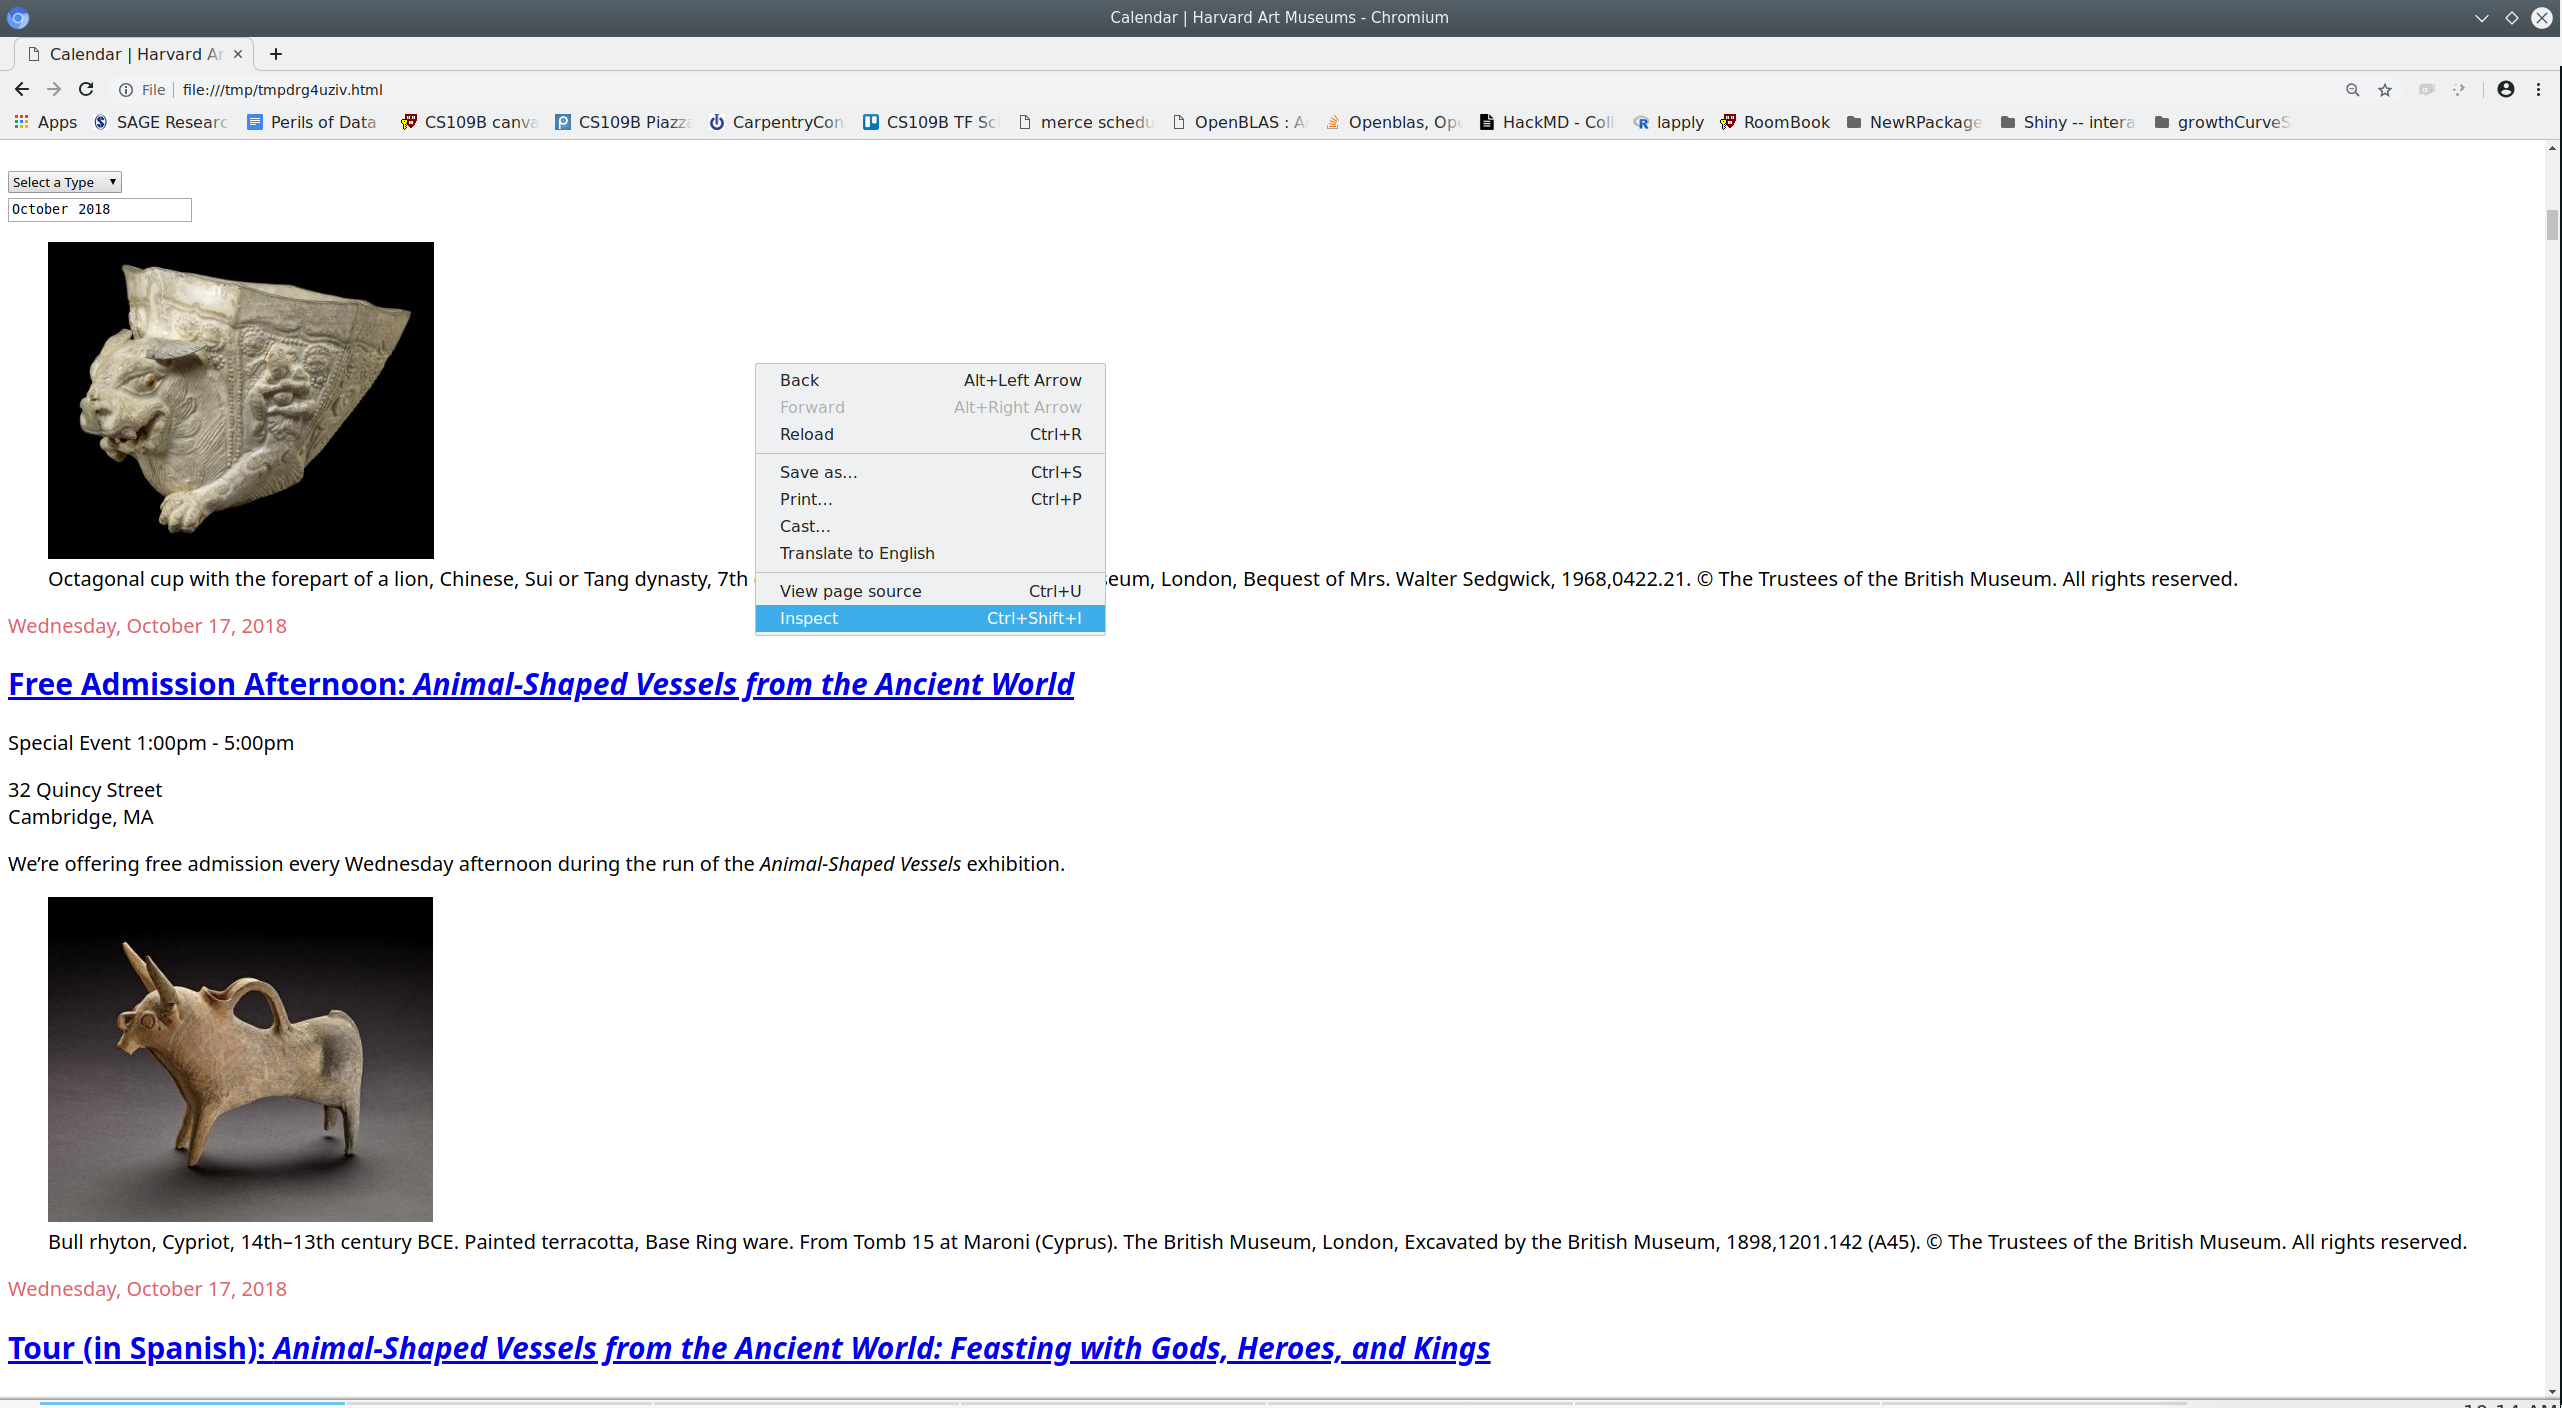
\includegraphics{Python/PythonWebScrape/images/dev_tools_right_click.png}
\caption{}
\end{figure}

\begin{figure}
\centering
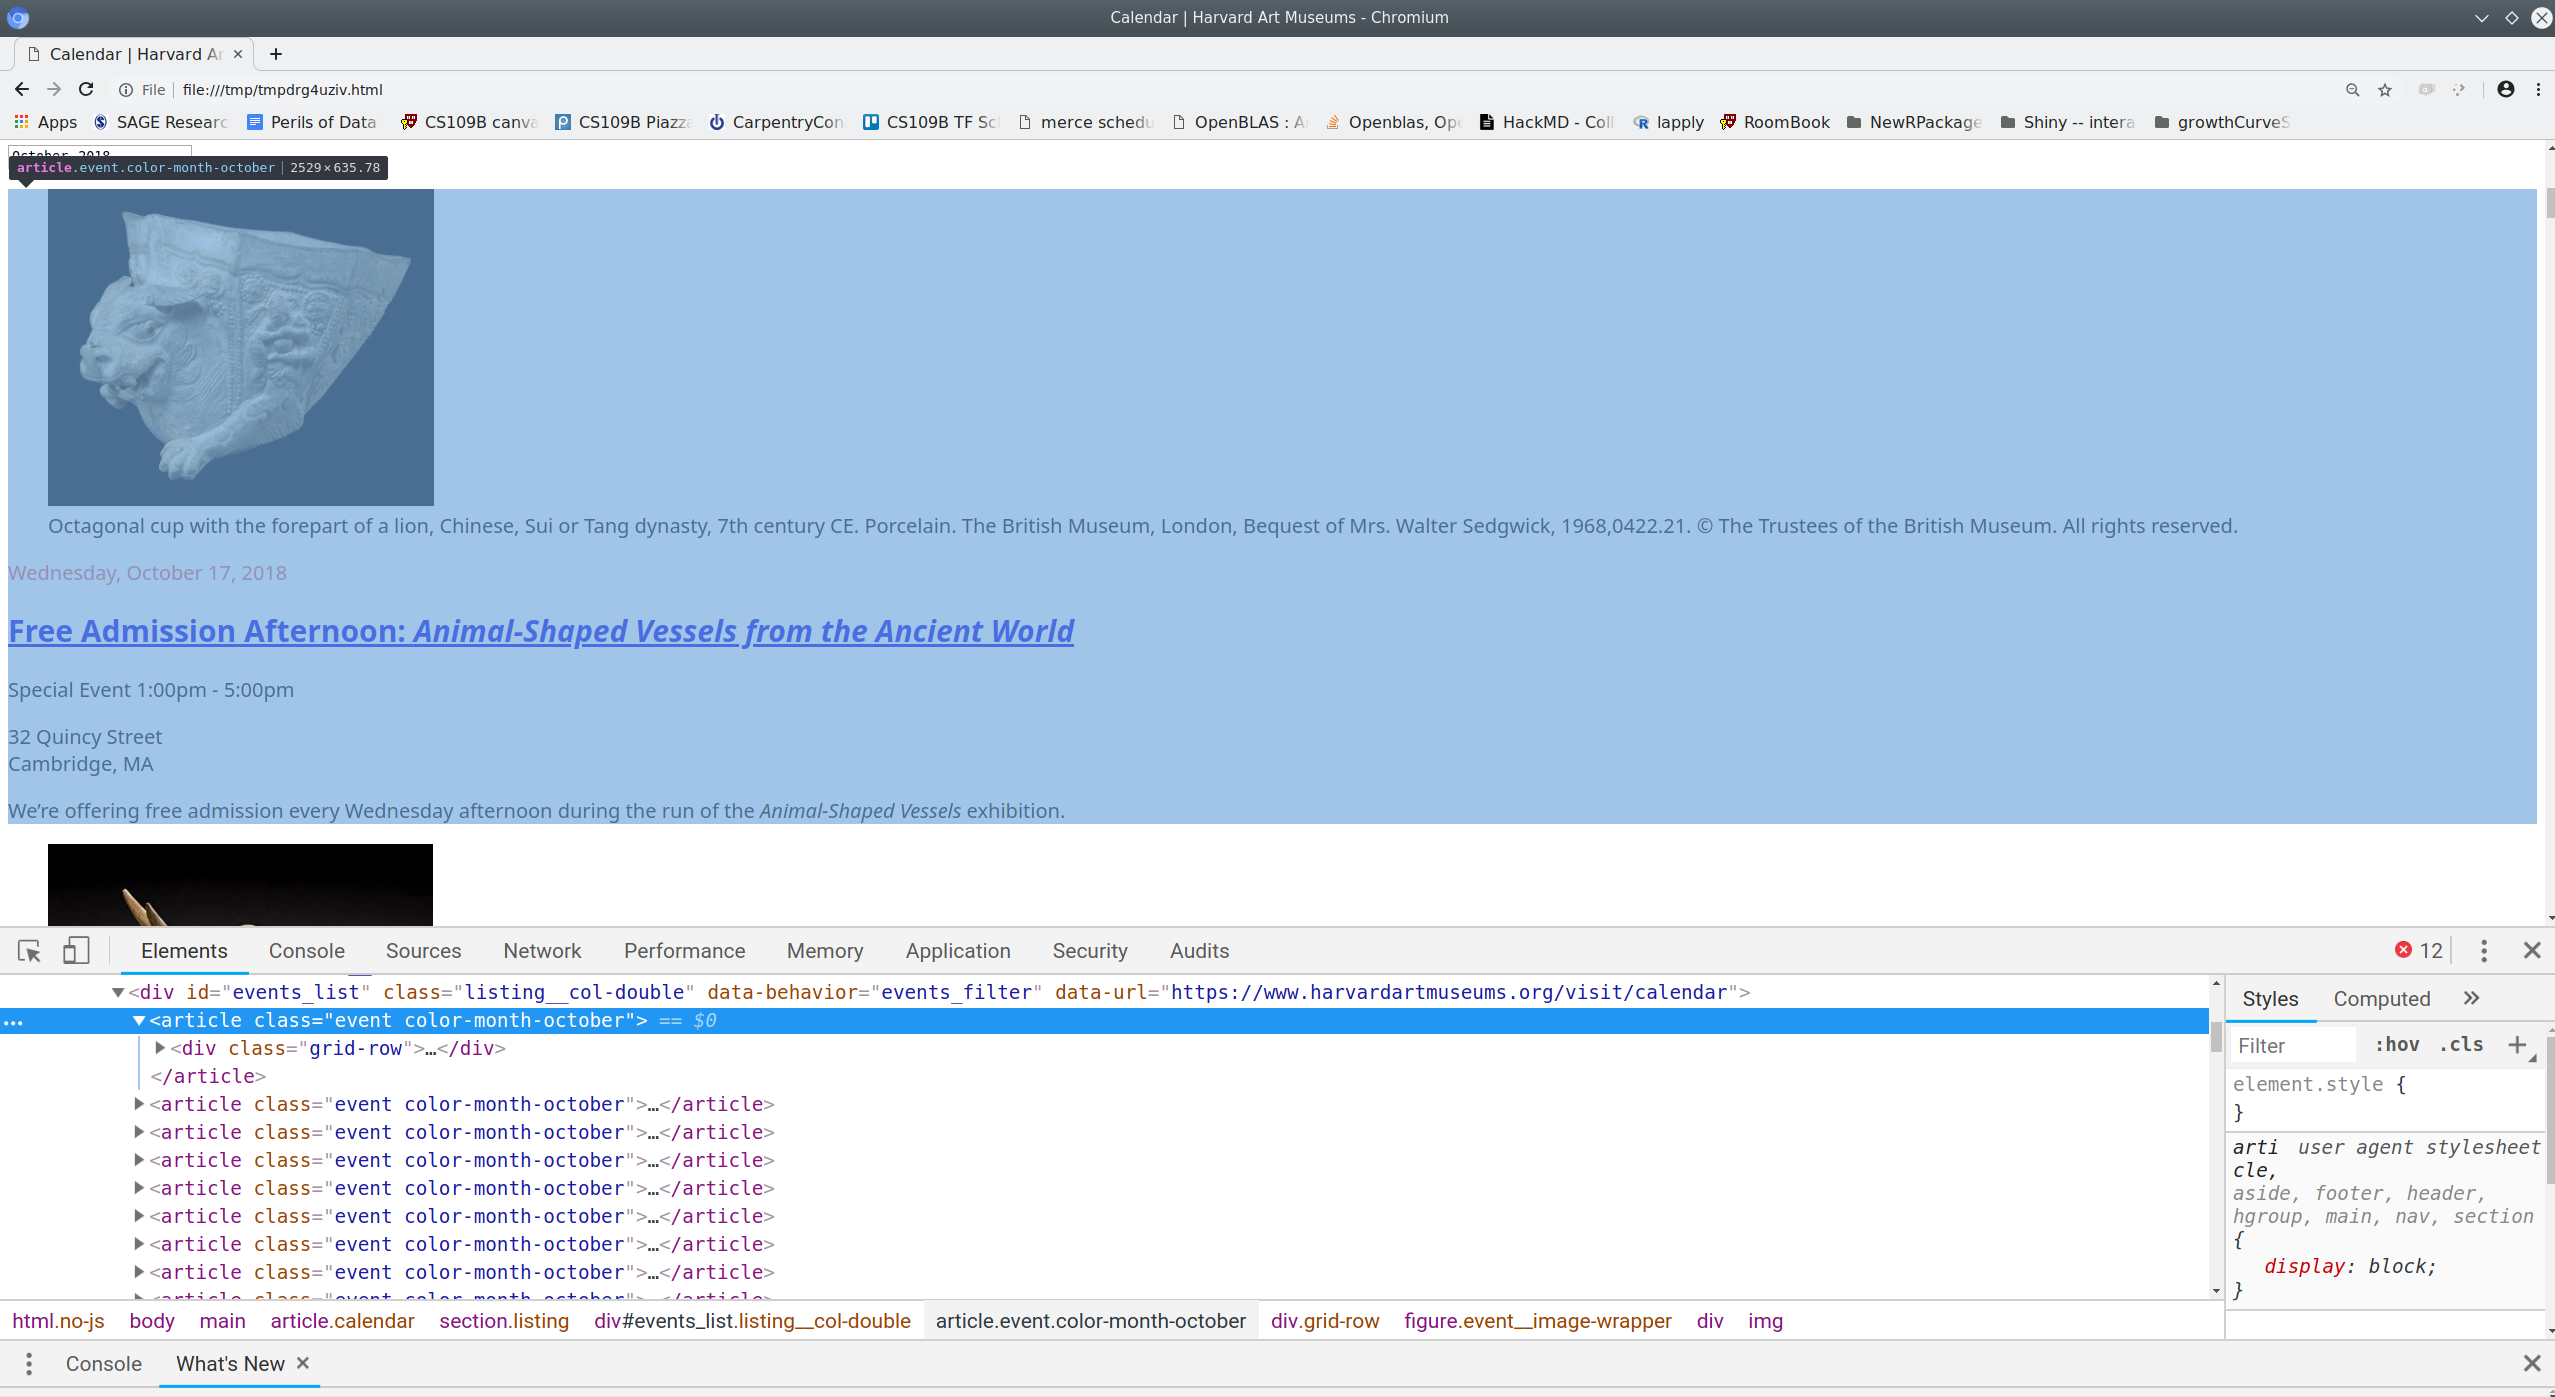
\includegraphics{Python/PythonWebScrape/images/dev_tools_inspect.png}
\caption{}
\end{figure}

Once we identify the element containing the information of interest we
can use our web browser to copy the \texttt{XPath} that uniquely
identifies that element.

\begin{figure}
\centering
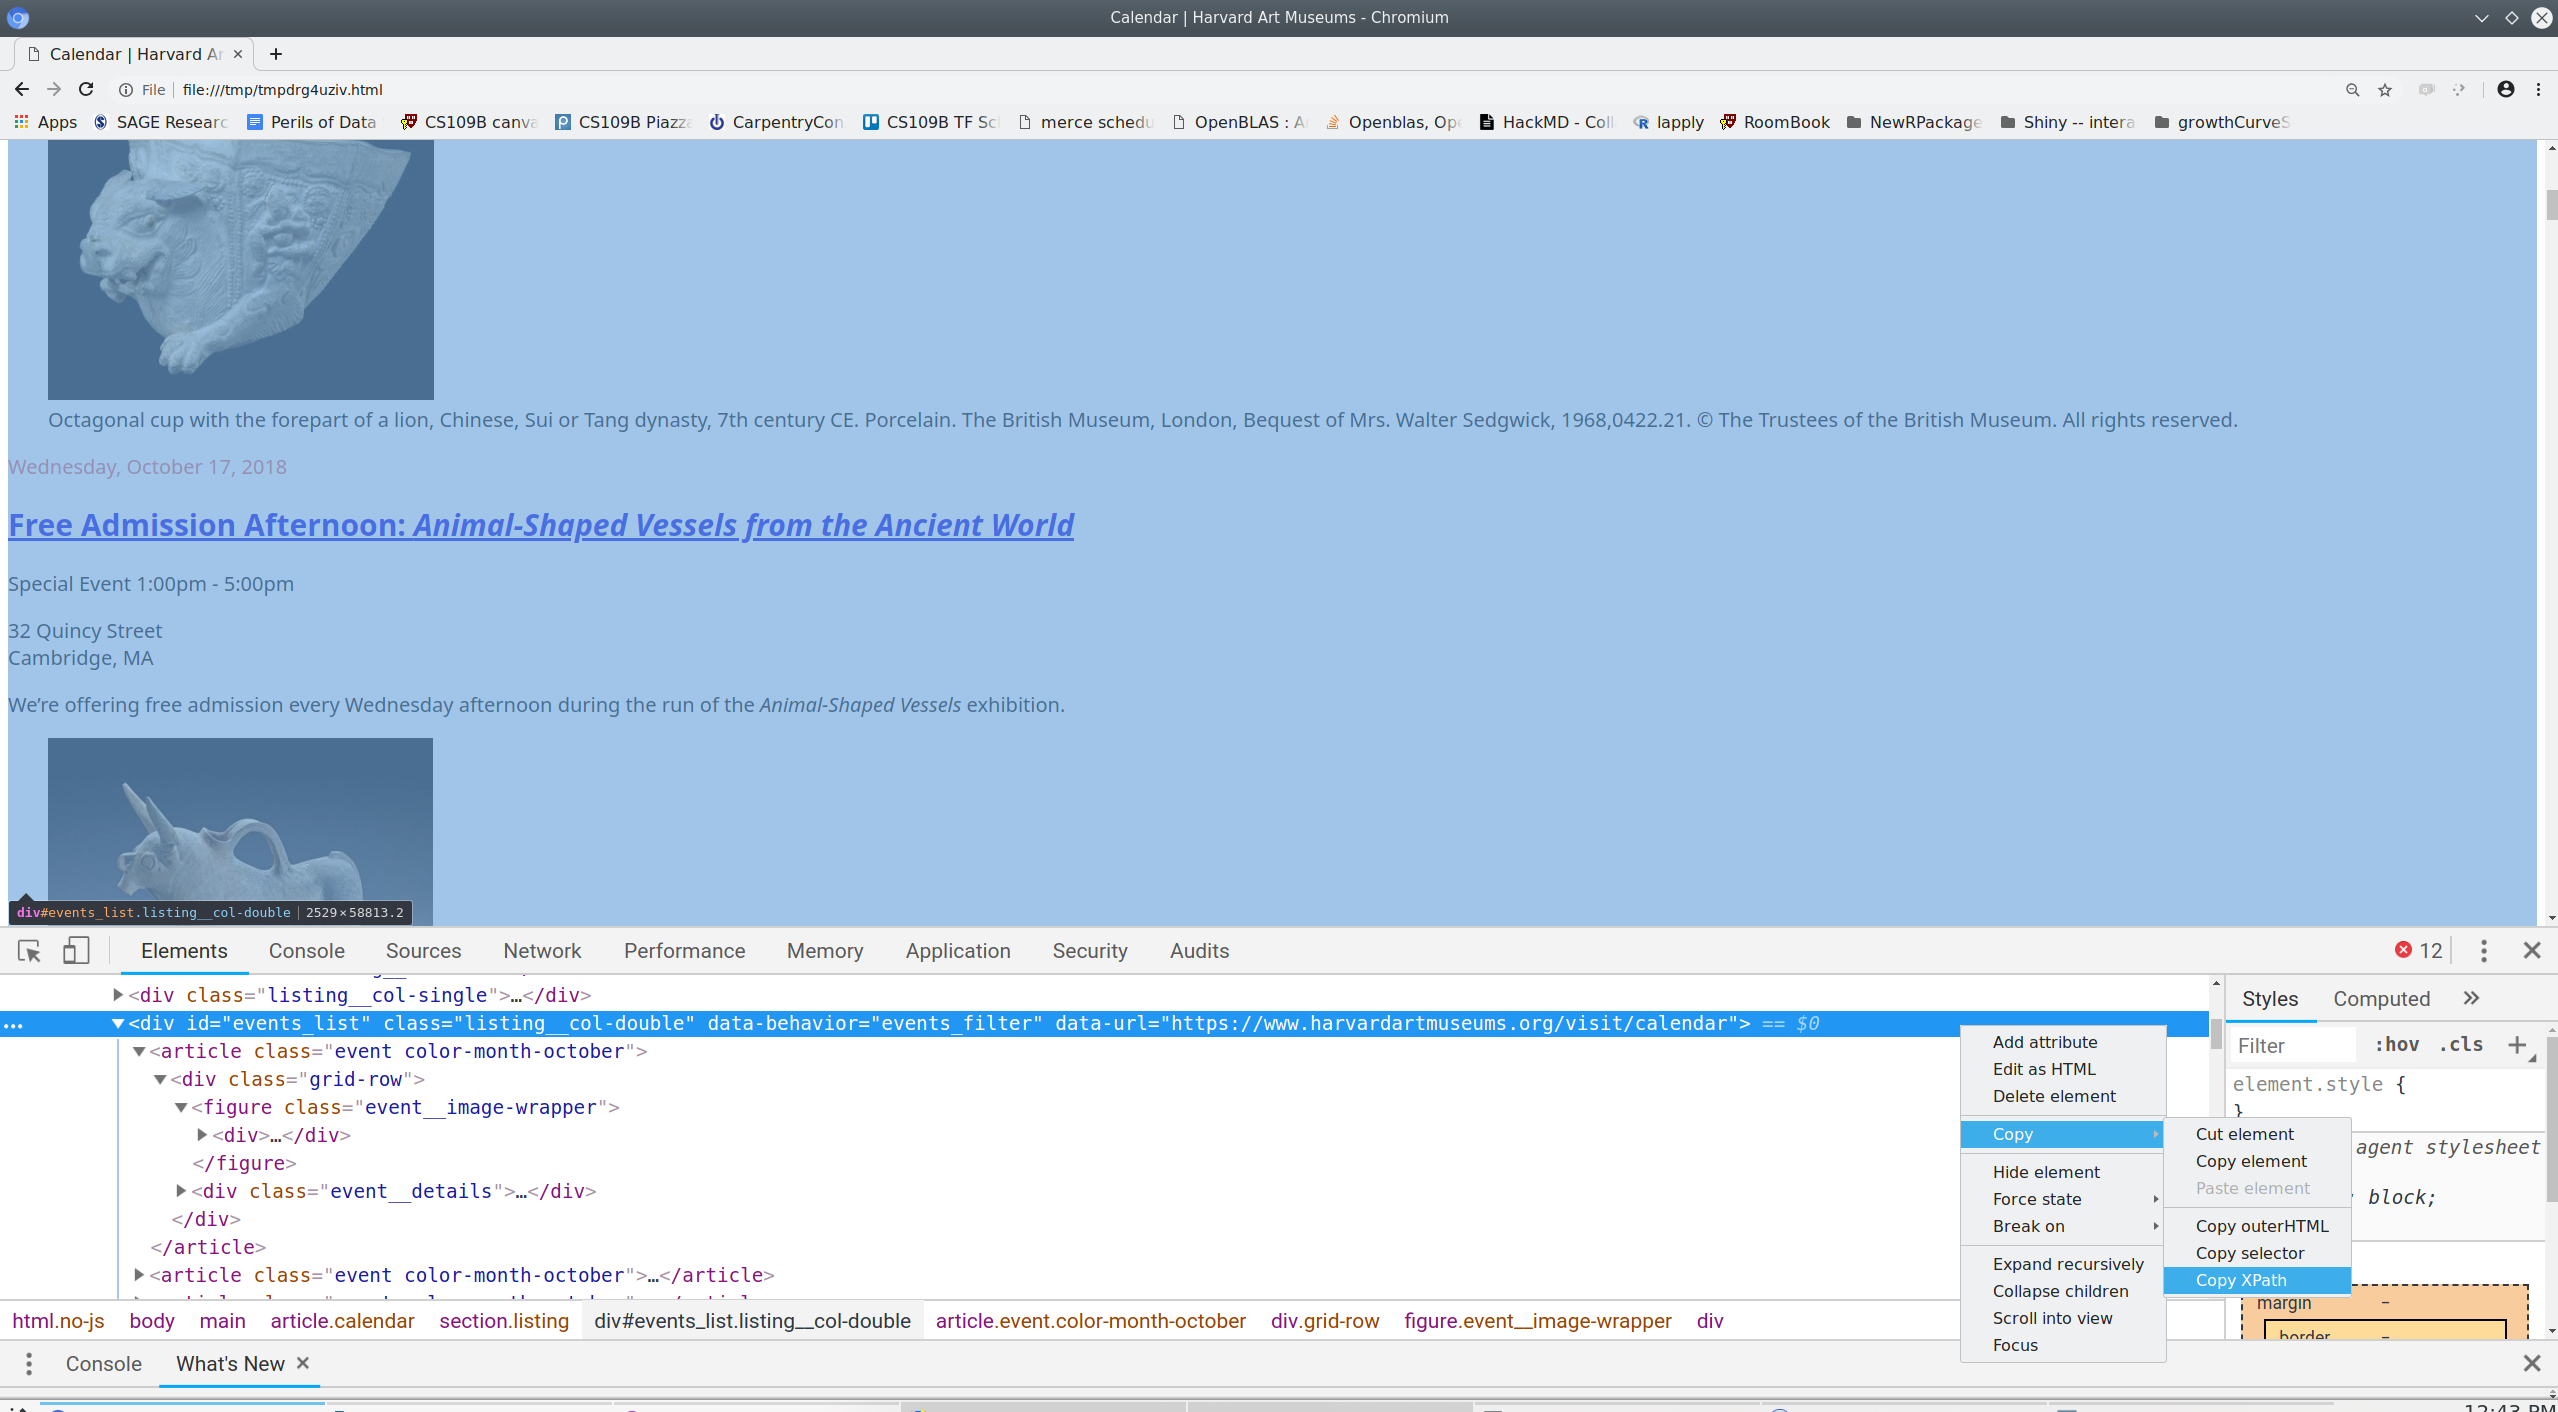
\includegraphics{Python/PythonWebScrape/images/dev_tools_xpath.png}
\caption{}
\end{figure}

Next we can use python to extract the element of interest:

\begin{Shaded}
\begin{Highlighting}[]
\NormalTok{events_list_html }\OperatorTok{=}\NormalTok{ events_html.xpath(}\StringTok{'//*[@id="events_list"]'}\NormalTok{)[}\DecValTok{0}\NormalTok{]}
\end{Highlighting}
\end{Shaded}

Once again we can use a web browser to inspect the HTML we're currently
working with, and to figure out what we want to extract from it. Let's
look at the first element in our events list.

\begin{Shaded}
\begin{Highlighting}[]
\NormalTok{first_event_html }\OperatorTok{=}\NormalTok{ events_list_html[}\DecValTok{0}\NormalTok{]}
\NormalTok{html.open_in_browser(first_event_html, encoding }\OperatorTok{=} \StringTok{'UTF-8'}\NormalTok{)}
\end{Highlighting}
\end{Shaded}

As before we can use our browser to find the xpath of the elements we
want.

\begin{figure}
\centering
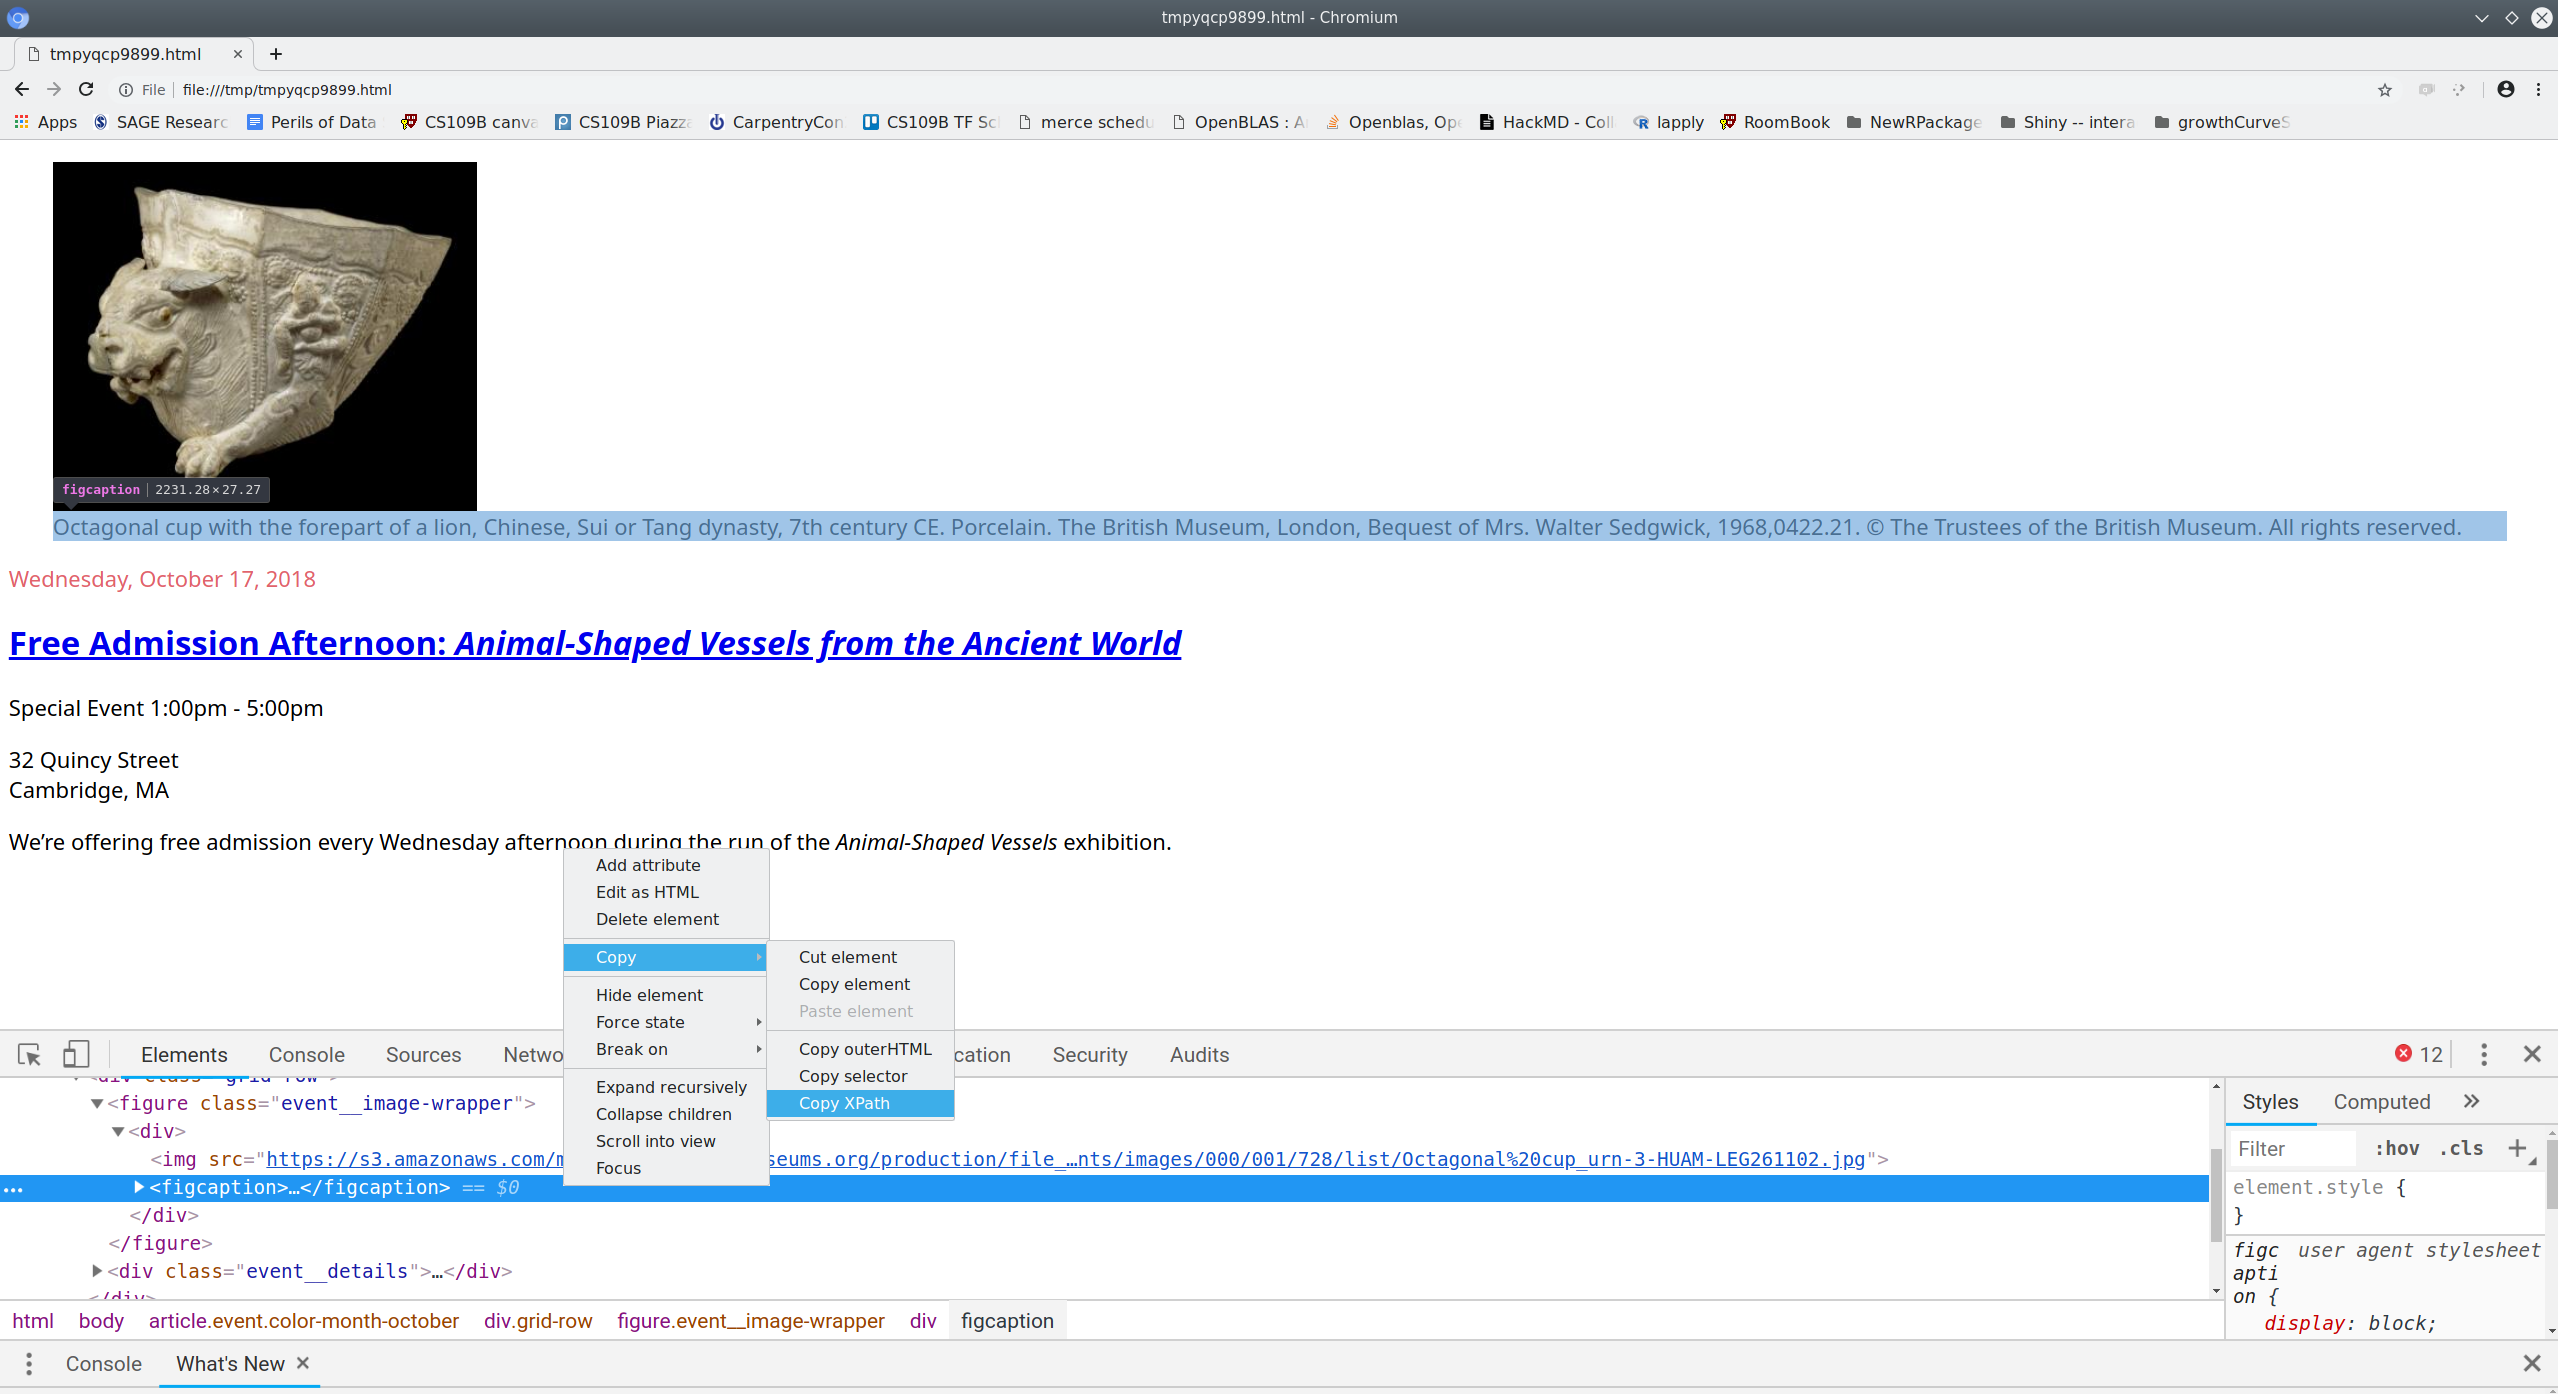
\includegraphics{Python/PythonWebScrape/images/dev_tools_figcaption.png}
\caption{}
\end{figure}

(Note that the \texttt{html.open\_in\_browser} function adds enclosing
\texttt{html} and \texttt{body} tags in order to create a complete web
page for viewing. This requires that we adjust the \texttt{xpath}
accordingly.)

By repeating this process for each element we want, we can build a list
of the xpaths to those elements.

\begin{Shaded}
\begin{Highlighting}[]
\NormalTok{elements_we_want }\OperatorTok{=}\NormalTok{ \{}\StringTok{'figcaption'}\NormalTok{: }\StringTok{'div/figure/div/figcaption'}\NormalTok{,}
                    \StringTok{'date'}\NormalTok{: }\StringTok{'div/div/header/time'}\NormalTok{,}
                    \StringTok{'title'}\NormalTok{: }\StringTok{'div/div/header/h2/a'}\NormalTok{,}
                    \StringTok{'time'}\NormalTok{: }\StringTok{'div/div/div/p[1]/time'}\NormalTok{,}
                    \StringTok{'localtion1'}\NormalTok{: }\StringTok{'div/div/div/p[2]/span/span[1]'}\NormalTok{,}
                    \StringTok{'location2'}\NormalTok{: }\StringTok{'div/div/div/p[2]/span/span[2]'}
\NormalTok{                    \}}
\end{Highlighting}
\end{Shaded}

Finally, we can iterate over the elements we want and extract them.

\begin{Shaded}
\begin{Highlighting}[]
\NormalTok{first_event_values }\OperatorTok{=}\NormalTok{ \{\}}
\ControlFlowTok{for}\NormalTok{ key }\KeywordTok{in}\NormalTok{ elements_we_want.keys():}
\NormalTok{    element }\OperatorTok{=}\NormalTok{ first_event_html.xpath(elements_we_want[key])[}\DecValTok{0}\NormalTok{]}
\NormalTok{    first_event_values[key] }\OperatorTok{=}\NormalTok{ element.text_content().strip()}

\BuiltInTok{print}\NormalTok{(first_event_values)}
\end{Highlighting}
\end{Shaded}

\subsection{Iterating to retrieve content from a list of HTML
elements}\label{iterating-to-retrieve-content-from-a-list-of-html-elements}

So far we've retrieved information only for the first event. To retrieve
data for all the events listed on the page we need to iterate over the
events. If we are very lucky, each event will have exactly the same
information structured in exactly the same way and we can simply extend
the code we wrote above to iterate over the events list.

Unfortunately not all these elements are available for every event, so
we need to take care to handle the case where one or more of these
elements is not available. We can do that by defining a function that
tries to retrieve a value and returns an empty string if it fails.

\begin{Shaded}
\begin{Highlighting}[]
\KeywordTok{def}\NormalTok{ get_event_info(event, path):}
    \ControlFlowTok{try}\NormalTok{:}
\NormalTok{        info }\OperatorTok{=}\NormalTok{ event.xpath(path)[}\DecValTok{0}\NormalTok{].text.strip()}
    \ControlFlowTok{except}\NormalTok{:}
\NormalTok{        info }\OperatorTok{=} \StringTok{''}
    \ControlFlowTok{return}\NormalTok{ info}
\end{Highlighting}
\end{Shaded}

Armed with this function we can iterate over the list of events and
extract the available information for each one.

\begin{Shaded}
\begin{Highlighting}[]
\NormalTok{all_event_values }\OperatorTok{=}\NormalTok{ \{\}}
\ControlFlowTok{for}\NormalTok{ key }\KeywordTok{in}\NormalTok{ elements_we_want.keys():}
\NormalTok{    key_values }\OperatorTok{=}\NormalTok{ []}
    \ControlFlowTok{for}\NormalTok{ event }\KeywordTok{in}\NormalTok{ events_list_html: }
\NormalTok{        key_values.append(get_event_info(event, elements_we_want[key]))}
\NormalTok{    all_event_values[key] }\OperatorTok{=}\NormalTok{ key_values}
\end{Highlighting}
\end{Shaded}

For convenience we can arrange these values in a pandas
\texttt{DataFrame} and save them as .csv files, just as we did with our
exhibitions data earlier.

\begin{Shaded}
\begin{Highlighting}[]
\NormalTok{all_event_values }\OperatorTok{=}\NormalTok{ pd.DataFrame.from_dict(all_event_values)}

\NormalTok{all_event_values.to_csv(}\StringTok{"all_event_values.csv"}\NormalTok{)}

\BuiltInTok{print}\NormalTok{(all_event_values)}
\end{Highlighting}
\end{Shaded}

\subsection{Exercise: parsing HTML}\label{exercise-parsing-html}

In this exercise you will retrieve information about the physical layout
of the Harvard Art Museums. The web page at
\url{https://www.harvardartmuseums.org/visit/floor-plan} contains this
information in HTML from.

\begin{enumerate}
\def\labelenumi{\arabic{enumi}.}
\tightlist
\item
  Using a web browser (Firefox or Chrome recommended) inspect the page
  at \texttt{https://www.harvardartmuseums.org/visit/floor-plan}. Copy
  the \texttt{XPath} to the element containing the list of level
  information. (HINT: the element if interest is a \texttt{ul}, i.e.,
  \texttt{unordered\ list}.)
\item
  Make a \texttt{get} request in Python to retrieve the web page at
  \url{https://www.harvardartmuseums.org/visit/floor-plan}. Extract the
  content from your request object and parse it using
  \texttt{html.fromstring} from the \texttt{lxml} library.
\item
  Use your web browser to find the \texttt{XPath}s to the facilities
  housed on level one. Use Python to extract the text from those
  \texttt{Xpath}s.
\item
  Bonus (optional): Write a \emph{loop} or \emph{list comprehension} in
  Python to retrieve data for all the levels.
\end{enumerate}

\section{Use Scrapy for large or complicated
projects}\label{use-scrapy-for-large-or-complicated-projects}

Scraping websites using the \texttt{requests} library to make GET and
POST requests, and the \texttt{lxml} library to process HTML is a good
way to learn basic web scraping techniques. It is a good choice for
small to medium size projects. For very large or complicated scraping
tasks the \texttt{scrapy} library offers a number of conveniences,
including asynchronously retrieval, session management, convenient
methods for extracting and storing values, and more. More information
about \texttt{scrapy} can be found at \url{https://doc.scrapy.org}.

\section{Use a browser driver as a last
resort}\label{use-a-browser-driver-as-a-last-resort}

It is sometimes necessary (or sometimes just easier) to use a web
browser as an intermediary rather than communicating directly with a web
service. This method has the advantage of being about to use the
javascript engine and session management features of a web browser; the
main disadvantage is that it is slower and tends to be more fragile than
using \texttt{requests} or \texttt{scrapy} to make requests directly
from python. For small scraping projects involving complicated sites
with CAPTHAs or lots of complicated javascript using a browser driver
can be a good option. More information is available at
\url{https://www.seleniumhq.org/docs/03_webdriver.jsp}.

\section{Wrap-up}\label{wrap-up-5}

\subsection{Feedback}\label{feedback-5}

Please take 60 seconds to fill out a very short feedback
\href{http://bit.ly/training_class_eval}{form}

\subsection{Resources}\label{resources-5}

\begin{itemize}
\tightlist
\item
  IQSS

  \begin{itemize}
  \tightlist
  \item
    \href{https://dss.iq.harvard.edu/workshop-materials}{Workshops}
  \item
    \href{https://dss.iq.harvard.edu/}{Data Science Services}
  \item
    \href{https://iqss.github.io/dss-rce/}{Research Computing
    Environment}
  \end{itemize}
\end{itemize}

\part{Stata}\label{part-stata}

\chapter{Stata Introduction}\label{stata-introduction}

\textbf{Topics}

\begin{itemize}
\tightlist
\item
  Assignment
\item
  Function arguments
\item
  Finding help
\item
  Reading data
\item
  Filtering and arranging data
\item
  Conditional operations
\item
  Saving data
\end{itemize}

\section{Setup}\label{setup-6}

\subsection{Software \& Materials}\label{software-materials-6}

Laptop users: you will need a copy of Stata installed on your machine.
Harvard FAS affiliates can install a licensed version from
\url{http://downloads.fas.harvard.edu/download}

\begin{itemize}
\tightlist
\item
  Find class materials at
  \url{http://tutorials.iq.harvard.edu/Stata/StataIntro.zip}
\item
  Download and extract to your desktop!
\end{itemize}

Laptop users: you will need a copy of Stata installed on your machine
Lab computer users: log in using your Harvard user name and password

Everyone:

\begin{itemize}
\tightlist
\item
  Find class materials at
  \url{http://tutorials.iq.harvard.edu/Stata/StataIntro.zip}
\item
  Download and extract to your desktop!
\end{itemize}

\subsection{Organization}\label{organization}

\begin{itemize}
\tightlist
\item
  Please feel free to ask questions at any point if they are relevant to
  the current topic (or if you are lost!)

  \begin{itemize}
  \tightlist
  \item
    There will be a Q\&A after class for more specific, personalized
    questions
  \end{itemize}
\item
  Collaboration with your neighbors is encouraged
\item
  If you are using a laptop, you will need to adjust paths accordingly
\item
  Make comments in your Do-file rather than on hand-outs

  \begin{itemize}
  \tightlist
  \item
    save on flash drive or email to yourself
  \end{itemize}
\end{itemize}

\subsection{Goals}\label{goals-6}

\begin{itemize}
\tightlist
\item
  This is an \textbf{introduction} to Stata
\item
  Assumes no/very little knowledge of Stata
\item
  Not appropriate for people already well familiar with Stata
\item
  Learning Objectives:

  \begin{itemize}
  \tightlist
  \item
    Familiarize yourself with the Stata interface
  \item
    Get data in and out of Stata
  \item
    Compute statistics and construct graphical displays
  \item
    Compute new variables and transformations
  \end{itemize}
\end{itemize}

\section{Why stata?}\label{why-stata}

\begin{itemize}
\tightlist
\item
  Used in a variety of disciplines
\item
  User-friendly
\item
  Great guides available on web (as well as in HMDC computer lab
  library)
\item
  Student and other discount packages available at reasonable cost
\end{itemize}

\subsection{Stata interface}\label{stata-interface}

\begin{figure}
\centering
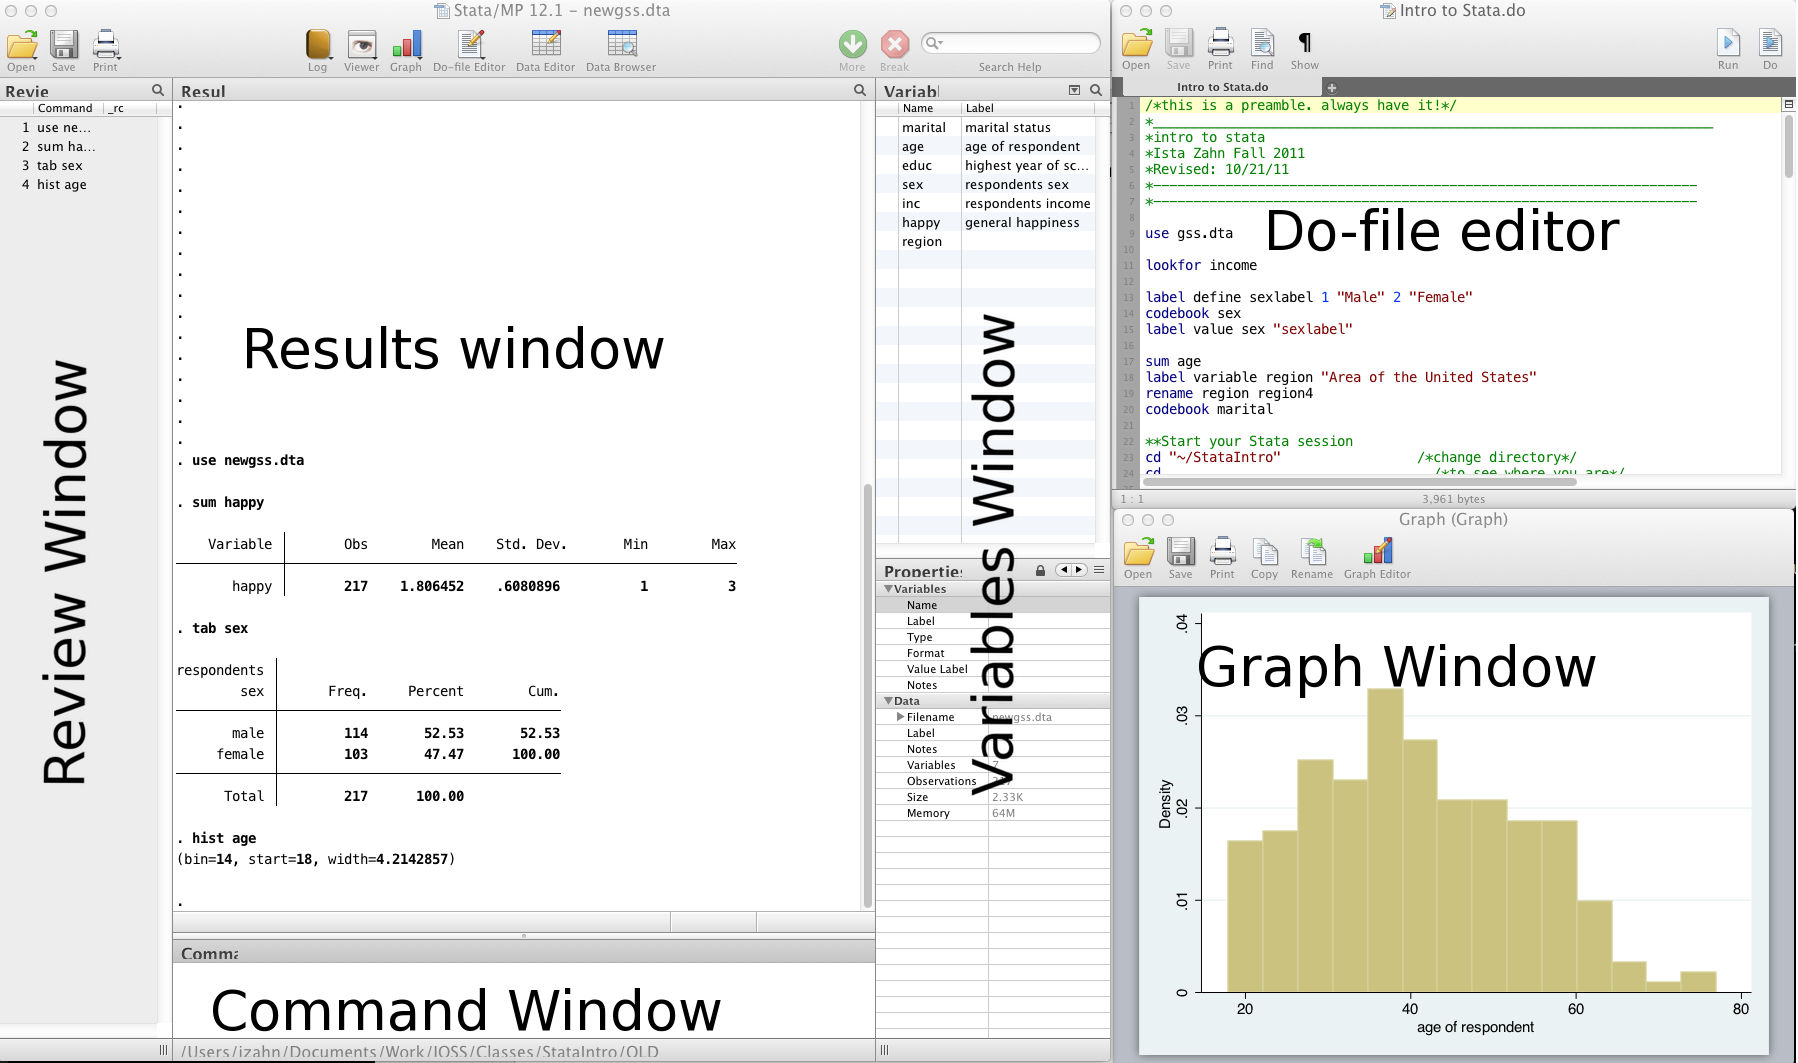
\includegraphics{Stata/StataIntro/images/StataInterface.png}
\caption{}
\end{figure}

\begin{itemize}
\tightlist
\item
  Review and Variable windows can be closed (user preference)
\item
  Command window can be shortened (recommended)
\end{itemize}

\subsection{Do-files}\label{do-files}

\begin{itemize}
\tightlist
\item
  You can type all the same commands into the Do-file that you would
  type into the command window
\item
  BUT\ldots{}the Do-file allows you to \textbf{save} your commands
\item
  Your Do-file should contain ALL commands you executed -- at least all
  the ``correct'' commands!
\item
  I recommend never using the command window or menus to make CHANGES to
  data
\item
  Saving commands in Do-file allows you to keep a written record of
  everything you have done to your data

  \begin{itemize}
  \tightlist
  \item
    Allows easy replication
  \item
    Allows you to go back and re-run commands, analyses and make
    modifications
  \end{itemize}
\end{itemize}

\subsection{Stata help}\label{stata-help}

To get help in Stata type \texttt{help} followed by topic or command,
e.g., \texttt{help\ codebook}.

\subsection{General Stata command
syntax}\label{general-stata-command-syntax}

Most Stata commands follow the same basic syntax:
\texttt{Command\ varlist,\ options}.

\subsection{Commenting and formatting
syntax}\label{commenting-and-formatting-syntax}

Start with comment describing your Do-file and use comments throughout

\begin{verbatim}
* Use '*' to comment a line and '//' for in-line comments

* Make Stata say hello:
disp "Hello " "World!" // 'disp' is short for 'display'
\end{verbatim}

\begin{verbatim}
Hello World!
\end{verbatim}

\begin{itemize}
\tightlist
\item
  Use \texttt{///} to break varlists over multiple lines:
\end{itemize}

\begin{verbatim}
disp "Hello" ///
     " World!"
\end{verbatim}

\begin{verbatim}
Hello World!
\end{verbatim}

\subsection{Let's get started}\label{lets-get-started}

\begin{itemize}
\tightlist
\item
  Launch the Stata program (MP or SE, does not matter unless doing
  computationally intensive work)

  \begin{itemize}
  \tightlist
  \item
    Open up a new Do-file
  \item
    Run our first Stata code!
  \end{itemize}
\end{itemize}

\begin{verbatim}
* change directory
// cd "C://Users/dataclass/Desktop/StataIntro"
\end{verbatim}

\section{Getting data into Stata}\label{getting-data-into-stata}

\subsection{Data file commands}\label{data-file-commands}

\begin{itemize}
\tightlist
\item
  Next, we want to open our data file
\item
  Open/save data sets with ``use'' and ``save'':
\end{itemize}

\begin{verbatim}
cd dataSets

// open the gss.dta data set
use gss.dta, clear

// save data file:
save newgss.dta, replace // "replace" option means OK to overwrite existing file
\end{verbatim}

\begin{verbatim}
/home/izahn/Documents/Work/Classes/IQSS_Stats_Workshops/Stata/StataIntro/dataSets


file newgss.dta saved
\end{verbatim}

\subsection{A note about path names}\label{a-note-about-path-names}

\begin{itemize}
\tightlist
\item
  If your path has no spaces in the name (that means all directories,
  folders, file names, etc. can have no spaces), you can write the path
  as is
\item
  If there are spaces, you need to put your pathname in quotes
\item
  Best to get in the habit of quoting paths
\end{itemize}

\subsection{Where's my data?}\label{wheres-my-data}

\begin{itemize}
\tightlist
\item
  Data editor (\textbf{browse})
\item
  Data editor (\textbf{edit})

  \begin{itemize}
  \tightlist
  \item
    Using the data editor is discouraged (why?)
  \end{itemize}
\item
  Always keep any changes to your data in your Do-file
\item
  Avoid temptation of making manual changes by viewing data via the
  browser rather than editor
\end{itemize}

\subsection{What if my data is not a Stata
file?}\label{what-if-my-data-is-not-a-stata-file}

\begin{itemize}
\tightlist
\item
  Import delimited text files
\end{itemize}

\begin{verbatim}
* import data from a .csv file
import delimited gss.csv, clear

* save data to a .csv file
export delimited gss_new.csv, replace
\end{verbatim}

\begin{verbatim}
Picked up _JAVA_OPTIONS: -Dawt.useSystemAAFontSettings=gasp -Dswing.aatext=true -Dsun.java2d.opengl=true
(7 vars, 451 obs)

file gss_new.csv saved
\end{verbatim}

\begin{itemize}
\tightlist
\item
  Import data from SAS and Excel
\end{itemize}

\begin{verbatim}
* import/export SAS xport files
clear
import sasxport gss.xpt
export sasxport gss_new, replace
\end{verbatim}

\begin{verbatim}
file gss_new.xpt saved
\end{verbatim}

\subsection{What if my data is from another statistical software
program?}\label{what-if-my-data-is-from-another-statistical-software-program}

\begin{itemize}
\tightlist
\item
  SPSS/PASW will allow you to save your data as a Stata file

  \begin{itemize}
  \tightlist
  \item
    Go to: file -\textgreater{} save as -\textgreater{} Stata (use most
    recent version available)
  \item
    Then you can just go into Stata and open it
  \end{itemize}
\item
  Another option is \textbf{StatTransfer}, a program that converts data
  from/to many common formats, including SAS, SPSS, Stata, and many more
\end{itemize}

\subsection{Exercise 1: Importing data}\label{exercise-1-importing-data}

\begin{enumerate}
\def\labelenumi{\arabic{enumi}.}
\tightlist
\item
  Save any work you've done so far. Close down Stata and open a new
  session.
\item
  Start Stata and open your \texttt{.do} file.
\item
  Change directory (\texttt{cd}) to the \texttt{dataSets} folder.
\item
  Try opening the following files:

  \begin{itemize}
  \tightlist
  \item
    A comma separated value file: gss.csv
  \item
    An Excel file: gss.xlsx
  \end{itemize}
\end{enumerate}

\section{Statistics and graphs}\label{statistics-and-graphs}

\subsection{Frequently used commands}\label{frequently-used-commands}

\begin{itemize}
\tightlist
\item
  Commands for reviewing and inspecting data:

  \begin{itemize}
  \tightlist
  \item
    describe // labels, storage type etc.
  \item
    sum // statistical summary (mean, sd, min/max etc.)
  \item
    codebook // storage type, unique values, labels
  \item
    list // print actuall values
  \item
    tab // (cross) tabulate variables
  \item
    browse // view the data in a spreadsheet-like window
  \end{itemize}
\item
  Examples
\end{itemize}

\begin{verbatim}
use gss.dta, clear

sum educ // statistical summary of education
\end{verbatim}

\begin{verbatim}
    Variable |        Obs        Mean    Std. Dev.       Min        Max
-------------+---------------------------------------------------------
        educ |        217    13.52995      3.0687          1         20
\end{verbatim}

\begin{verbatim}
codebook region // information about how region is coded
\end{verbatim}

\begin{verbatim}
---------------------------------------------------------------------------------------------------------------------------------------------------------------------------------------------------------------------------------------------------------------
region                                                                                                                                                                                                                                              (unlabeled)
---------------------------------------------------------------------------------------------------------------------------------------------------------------------------------------------------------------------------------------------------------------

                  type:  string (str5)

         unique values:  4                        missing "":  0/217

            tabulation:  Freq.  Value
                            54  "east"
                            48  "north"
                            48  "south"
                            67  "west"
\end{verbatim}

\begin{verbatim}
tab sex // numbers of male and female participants
\end{verbatim}

\begin{verbatim}
respondents |
        sex |      Freq.     Percent        Cum.
------------+-----------------------------------
       male |        114       52.53       52.53
     female |        103       47.47      100.00
------------+-----------------------------------
      Total |        217      100.00
\end{verbatim}

\begin{itemize}
\tightlist
\item
  If you run these commands without specifying variables, Stata will
  produce output for every variable
\end{itemize}

\subsection{Basic graphing commands}\label{basic-graphing-commands}

\begin{itemize}
\tightlist
\item
  Univariate distribution(s) using \textbf{hist}
\end{itemize}

\begin{verbatim}
  /* Histograms */
  hist educ
\end{verbatim}

\begin{verbatim}
(bin=14, start=1, width=1.3571429)
\end{verbatim}

\begin{verbatim}
  // histogram with normal curve; see 'help hist' for other options
  hist age, normal  
\end{verbatim}

\begin{verbatim}
(bin=14, start=18, width=4.2142857)
\end{verbatim}

\begin{itemize}
\tightlist
\item
  View bivariate distributions with scatterplots
\end{itemize}

\begin{verbatim}
   /* scatterplots */
   twoway (scatter educ age)
\end{verbatim}

\begin{verbatim}
graph matrix educ age inc
\end{verbatim}

\subsection{\texorpdfstring{The ``by''
command}{The by command}}\label{the-by-command}

\begin{itemize}
\tightlist
\item
  Sometimes, you'd like to generate output based on different categories
  of a grouping variable
\item
  The ``by'' command does just this
\end{itemize}

\begin{verbatim}
* By Processing
bysort sex: tab happy // tabulate happy separately for men and women
\end{verbatim}

\begin{verbatim}
---------------------------------------------------------------------------------------------------------------------------------------------------------------------------------------------------------------------------------------------------------------
-> sex = male

      general |
    happiness |      Freq.     Percent        Cum.
--------------+-----------------------------------
   very happy |         32       28.07       28.07
 pretty happy |         68       59.65       87.72
not too happy |         14       12.28      100.00
--------------+-----------------------------------
        Total |        114      100.00

---------------------------------------------------------------------------------------------------------------------------------------------------------------------------------------------------------------------------------------------------------------
-> sex = female

      general |
    happiness |      Freq.     Percent        Cum.
--------------+-----------------------------------
   very happy |         33       32.04       32.04
 pretty happy |         61       59.22       91.26
not too happy |          9        8.74      100.00
--------------+-----------------------------------
        Total |        103      100.00
\end{verbatim}

\begin{verbatim}
bysort marital: sum educ // summarize eudcation by marital status
\end{verbatim}

\begin{verbatim}
---------------------------------------------------------------------------------------------------------------------------------------------------------------------------------------------------------------------------------------------------------------
-> marital = married

    Variable |        Obs        Mean    Std. Dev.       Min        Max
-------------+---------------------------------------------------------
        educ |        103    13.65049    3.374381          1         20

---------------------------------------------------------------------------------------------------------------------------------------------------------------------------------------------------------------------------------------------------------------
-> marital = widowed

    Variable |        Obs        Mean    Std. Dev.       Min        Max
-------------+---------------------------------------------------------
        educ |          6    12.33333     1.36626         11         15

---------------------------------------------------------------------------------------------------------------------------------------------------------------------------------------------------------------------------------------------------------------
-> marital = divorced

    Variable |        Obs        Mean    Std. Dev.       Min        Max
-------------+---------------------------------------------------------
        educ |         39    13.46154    2.501012          6         19

---------------------------------------------------------------------------------------------------------------------------------------------------------------------------------------------------------------------------------------------------------------
-> marital = separate

    Variable |        Obs        Mean    Std. Dev.       Min        Max
-------------+---------------------------------------------------------
        educ |          9    12.11111    2.803767          6         14

---------------------------------------------------------------------------------------------------------------------------------------------------------------------------------------------------------------------------------------------------------------
-> marital = never ma

    Variable |        Obs        Mean    Std. Dev.       Min        Max
-------------+---------------------------------------------------------
        educ |         60        13.7    3.004516          6         20
\end{verbatim}

\subsection{Exercise 2: Descriptive
statistics}\label{exercise-2-descriptive-statistics}

\begin{enumerate}
\def\labelenumi{\arabic{enumi}.}
\tightlist
\item
  Use the dataset, gss.dta
\item
  Examine a few selected variables using the describe, sum and codebook
  commands
\item
  Tabulate the variable, ``marital,'' with and without labels
\item
  Summarize the variable, ``income'' by marital status
\item
  Cross-tabulate marital with region
\item
  Summarize the variable \texttt{happy} for married individuals only
\end{enumerate}

\section{Basic data management}\label{basic-data-management}

\subsection{Labels}\label{labels}

\begin{itemize}
\tightlist
\item
  You never know why and when your data may be reviewed
\item
  ALWAYS label every variable no matter how insignificant it may seem
\item
  Stata uses two sets of labels: \textbf{variable labels} and
  \textbf{value labels}
\item
  Variable labels are very easy to use -- value labels are a little more
  complicated
\end{itemize}

\subsection{Variable and value labels}\label{variable-and-value-labels}

\begin{itemize}
\tightlist
\item
  Variable labels
\end{itemize}

\begin{verbatim}
  /* Labelling and renaming */
  // Label variable inc "household income"
  label var inc "household income"

  // change the name 'educ' to 'education'
  rename educ education

  // you can search names and labels with 'lookfor' 
  lookfor household
\end{verbatim}

\begin{verbatim}
              storage   display    value
variable name   type    format     label      variable label
---------------------------------------------------------------------------------------------------------------------------------------------------------------------------------------------------------------------------------------------------------------
inc             byte    %8.0g      rincom06   household income
\end{verbatim}

\begin{itemize}
\tightlist
\item
  Value labels are a two step process: define a value label, then assign
  defined label to variable(s)
\end{itemize}

\begin{verbatim}
  /*define a value label for sex */
  label define mySexLabel 1 "Male" 2 "Female"
  /* assign our label set to the sex variable*/
  label val sex  mySexLabel
\end{verbatim}

\subsection{Exercise 3: Variable labels and value
labels}\label{exercise-3-variable-labels-and-value-labels}

\begin{enumerate}
\def\labelenumi{\arabic{enumi}.}
\tightlist
\item
  Open the data set \textbf{gss.csv}
\item
  Familiarize yourself with the data using describe, sum, etc.
\item
  Rename and label variables using the following codebook:
\end{enumerate}

\begin{longtable}[]{@{}lll@{}}
\toprule
\textbf{var} & \textbf{rename to} & \textbf{label with}\tabularnewline
\midrule
\endhead
v1 & marital & marital status\tabularnewline
v2 & age & age of respondent\tabularnewline
v3 & educ & education\tabularnewline
v4 & sex & respondent's sex\tabularnewline
v5 & inc & household income\tabularnewline
v6 & happy & general happiness\tabularnewline
v7 & region & region of interview\tabularnewline
\bottomrule
\end{longtable}

\begin{enumerate}
\def\labelenumi{\arabic{enumi}.}
\tightlist
\item
  Add value labels to your ``marital'' variable using this codebook:
\end{enumerate}

\begin{longtable}[]{@{}ll@{}}
\toprule
\textbf{value} & \textbf{label}\tabularnewline
\midrule
\endhead
1 & ``married''\tabularnewline
2 & ``widowed''\tabularnewline
3 & ``divorced''\tabularnewline
4 & ``separated''\tabularnewline
5 & ``never married''\tabularnewline
\bottomrule
\end{longtable}

\subsection{Working on subsets}\label{working-on-subsets}

\begin{itemize}
\tightlist
\item
  It is often useful to select just those rows of your data where some
  condition holds--for example select only rows where sex is 1 (male)
\item
  The following operators allow you to do this:
\end{itemize}

\begin{longtable}[]{@{}ll@{}}
\toprule
Operator & Meaning\tabularnewline
\midrule
\endhead
== & equal to\tabularnewline
!= & not equal to\tabularnewline
\textgreater{} & greater than\tabularnewline
\textgreater{}= & greater than or equal to\tabularnewline
\textless{} & less than\tabularnewline
\textless{}= & less than or equal to\tabularnewline
\& & and\tabularnewline
& or\tabularnewline
\bottomrule
\end{longtable}

\begin{itemize}
\tightlist
\item
  Note the double equals signs for testing equality
\end{itemize}

\subsection{Generating and replacing
variables}\label{generating-and-replacing-variables}

\begin{itemize}
\tightlist
\item
  Create new variables using ``gen''
\end{itemize}

\begin{verbatim}
  // create a new variable named mc_inc
  //   equal to inc minus the mean of inc
  gen mc_inc = inc - 15.37  
\end{verbatim}

\begin{itemize}
\tightlist
\item
  Sometimes useful to start with blank values and fill them in based on
  values of existing variables
\end{itemize}

\begin{verbatim}
  /* the 'generate and replace' strategy */ 
  // generate a column of missings
  gen age_wealth = .
  // Next, start adding your qualifications
  replace age_wealth=1 if age<30 & inc < 10
  replace age_wealth=2 if age<30 & inc > 10
  replace age_wealth=3 if age>30 & inc < 10
  replace age_wealth=4 if age>30 & inc > 10

  // conditions can also be combined with "or"
  gen young=0
  replace young=1 if age_wealth==1 | age_wealth==2
\end{verbatim}

\begin{verbatim}
(217 missing values generated)

(19 real changes made)

(26 real changes made)

(22 real changes made)

(134 real changes made)


(45 real changes made)
\end{verbatim}

\subsection{Exercise 4: Manipulating
variables}\label{exercise-4-manipulating-variables}

\begin{enumerate}
\def\labelenumi{\arabic{enumi}.}
\tightlist
\item
  Use the dataset, gss.dta
\item
  Generate a new variable, age2 equal to age squared
\item
  Generate a new ``high income'' variable that will take on a value of
  ``1'' if a person has an income value greater than ``15'' and ``0''
  otherwise
\item
  Generate a new divorced/separated dummy variable that will take on a
  value of ``1'' if a person is either divorced or separated and ``0''
  otherwise
\end{enumerate}

\section{Wrap-up}\label{wrap-up-6}

\subsection{Feedback}\label{feedback-6}

Please take 60 seconds to fill out a very short feedback
\href{http://bit.ly/training_class_eval}{form}

\subsection{Resources}\label{resources-6}

\begin{itemize}
\tightlist
\item
  IQSS

  \begin{itemize}
  \tightlist
  \item
    \href{https://dss.iq.harvard.edu/workshop-materials}{Workshops}
  \item
    \href{https://dss.iq.harvard.edu/}{Data Science Services}
  \item
    \href{https://iqss.github.io/dss-rce/}{Research Computing
    Environment}
  \end{itemize}
\end{itemize}


\end{document}
